%!TEX TS-program = pdflatex
% dissertation.tex -- main dissertation file
%
% Wisconsin dissertation template
% Copyright (c) 2008-2009 William C. Benton.  All rights reserved.
%
% This program can redistributed and/or modified under the terms
% of the LaTeX Project Public License Distributed from CTAN
% archives in directory macros/latex/base/lppl.txt; either
% version 1 of the License, or (at your option) any later version.
%
% This program includes other software that is licensed under the
% terms of the LPPL and the Perl Artistic License; see README for details.
%
% You, the user, still hold the copyright to any document you produce
% with this software (like your dissertation).
%

%%% You'll want ``oneside'' for the deposit version, but probably not for any versions that don't need to meet the UW requirements
\documentclass[12pt,oneside,letterpaper]{memoir}
\setlrmarginsandblock{1.3in}{*}{1}
\checkandfixthelayout

\setsecnumdepth{subsection}
\maxtocdepth{subsection}

% preamble.tex -- packages to include
%
% Wisconsin dissertation template
% Copyright (c) 2008 William C. Benton.  All rights reserved.
%
% This program can redistributed and/or modified under the terms
% of the LaTeX Project Public License Distributed from CTAN
% archives in directory macros/latex/base/lppl.txt; either
% version 1 of the License, or (at your option) any later version.
%
% This program includes other software that is licensed under the
% terms of the LPPL and the Perl Artistic License; see README for details.
%
% You, the user, still hold the copyright to any document you produce
% with this software (like your dissertation).

%% You should use natbib
\IfFileExists{natbib.sty}{%
\usepackage{natbib}%
}{}

%% You probably need appendix, if you want appendices
\IfFileExists{appendix.sty}{%
\usepackage{appendix}%
}{}

%% the spacing in memoir is weird, you'll need to use this
\DisemulatePackage{setspace}
\usepackage[onehalfspacing]{setspace}

%% List setup; the ``hanglist`` environment will allow you to have
%% nicely-typeset enumerated lists (i.e. with the numbers hanging in
%% the margins).  You need at least version 2.1 of enumitem.sty.  If
%% you don't have enumitem installed at all, hanglist will just be an
%% alias for enumerate.
\IfFileExists{enumitem.sty}{%
\usepackage[loadonly]{enumitem}[2007/06/30]%
\newlist{hanglist}{enumerate}{1}% 
\setlist[hanglist]{label=\arabic*.}%
\setlist[hanglist,1]{leftmargin=0pt}%
}{%
\newenvironment{hanglist}{\begin{enumerate}}{\end{enumerate}}%
}

%% Comment out any of these that you don't want
\usepackage{amssymb}
\usepackage{amsmath}
\usepackage{amsthm}
%\usepackage{theorem}
\usepackage[colorlinks=true]{hyperref}

\IfFileExists{mathpartir.sty}{%
\usepackage{mathpartir}%
}{}

%%%%% LISTINGS package and setup
\IfFileExists{listings.sty}{%
\usepackage{listings}%
}{}



%% Get rid of ugly borders around PDF hyperlinks (e.g. for cross-references, bib entries, or URLs)
\hypersetup{pdfborder = 0 0 0}

%% You want microtype.
\IfFileExists{microtype.sty}{%
\usepackage[protrusion=true,expansion=true]{microtype}%
}{}

%\pagestyle{thesisdraft}

% Surround parts of graphics with box
\usepackage{boxedminipage}

%% booktabs (thx to Nate Rosenblum for bringing this beautiful package
%% to my attention)
\IfFileExists{booktabs.sty}{%
\usepackage{booktabs}%
}{}

% This is now the recommended way for checking for PDFLaTeX:
\usepackage{ifpdf}

%% Avoid ugly "Type 3" fonts
\usepackage{lmodern}
\usepackage[LY1]{fontenc}

%% Substitute your favorite serif and sans fonts here....
\IfFileExists{tgpagella.sty}{%
% TeX Gyre pagella, like Palatino
\usepackage{tgpagella}%
}{}

\usepackage[LY1]{eulervm}

\ifpdf
\usepackage[pdftex]{graphicx}
\else
\usepackage{graphicx}
\fi

\usepackage{makeidx}
\makeindex

{\theoremstyle{plain}
\newtheorem{thm}{Theorem}[chapter]
\newtheorem{cor}[thm]{Corollary}
\newtheorem{define}[thm]{Definition}
\newtheorem{exmpl}[thm]{Example}
}
{\theoremstyle{remark}
\newtheorem{rmk}[thm]{Remark}
}

\newtheoremstyle{customsty1}
{3pt}%
{3pt}%
{}% --- body font
{}% --- indent amount
{\bfseries}% --- Theorem head font
{:}% --- Punctuation after head
{.5em}% --- space after head
{}% --- theorem head spec (can be left empty, meaning 'normal')

% Define 'newtheorems' that use ``customsty1''
{\theoremstyle{customsty1} 
}


%%% NB: the ``deposit'' chapter- and page- styles should conform to UW
%%% requirements.  If you are producing a pretty version of your
%%% dissertation for web use later, you will certainly want to make
%%% your own chapter and page styles.

\makechapterstyle{deposit}{%
  \renewcommand{\chapterheadstart}{}
  \renewcommand{\printchaptername}{}
  \renewcommand{\chapternamenum}{}
  \renewcommand{\printchapternum}{\parbox{2em}{\MakeLowercase{\Large\scshape\thechapter{}}} }
  \renewcommand{\afterchapternum}{}
  \renewcommand{\printchaptertitle}[1]{%
  \raggedright\Large\scshape\MakeLowercase{##1}}
  \renewcommand{\afterchaptertitle}{%
  \vskip\onelineskip \hrule\vskip\onelineskip}
}

\makepagestyle{deposit}
 
\makeatletter
 
\renewcommand{\chaptermark}[1]{\markboth{#1}{}}
\renewcommand{\sectionmark}[1]{\markboth{#1}{}}
 
\makeevenfoot{deposit}{}{}{}
\makeoddfoot{deposit}{}{}{}
\makeevenhead{deposit}{\thepage}{}{}
\makeoddhead{deposit}{}{}{\thepage}
\makeatother

%%% set up page numbering for chapter pages to satisfy UW requirements
%%% NB: You will want to delete until the ``SNIP'' mark if you are
%%% making a ``nice'' copy
\copypagestyle{chapter}{plain}
\makeoddfoot{chapter}{}{}{}
\makeevenhead{chapter}{\thepage}{}{}
\makeoddhead{chapter}{}{}{\thepage}
%%% SNIP

%%% bib nonsense
\makeatletter
\newenvironment{wb-bib}[1]{%
  \chapter*{references}
\ifnobibintoc\else 
\phantomsection 
\addcontentsline{toc}{chapter}{References} 
\fi 
\prebibhook
  \begin{bibitemlist}{#1}}{\end{bibitemlist}\postbibhook}

\AtBeginDocument{%
  \@ifpackageloaded{natbib}{% natbib is loaded
    \addtodef{\endthebibliography}{}{\vskip-\lastskip\postbibhook}
    \@ifpackagewith{natbib}{sectionbib}{% with sectionbib option
      \renewcommand{\bibsection}{\@memb@bsec}}%
      {\renewcommand{\bibsection}{\@memb@bchap}}}%
  {}
  \@ifpackagewith{chapterbib}{sectionbib}{%
    \renewcommand{\sectionbib}[2]{}
    \renewcommand{\bibsection}{\@memb@bsec}}{}
}
\makeatother

\hypersetup{pageanchor=false}
% defs.tex -- wbepi environment for chapter epigraphs and other useful defs.
%
% Wisconsin dissertation template
% Copyright (c) 2008 William C. Benton.  All rights reserved.
%
% This program can redistributed and/or modified under the terms
% of the LaTeX Project Public License Distributed from CTAN
% archives in directory macros/latex/base/lppl.txt; either
% version 1 of the License, or (at your option) any later version.
%
% This program includes other software that is licensed under the
% terms of the LPPL and the Perl Artistic License; see README for details.
%
% You, the user, still hold the copyright to any document you produce
% with this software (like your dissertation).


%% put lstnewenvironment declarations here, if you're using listings

%% end lstnewenvironment declarations

%% I put convenience definitions that will go in several chapters here

%%%%% begin convenience definitions

\makeatletter
\newcommand{\wb@episource}{}
\newenvironment{wbepi}[1]{\begin{quote}\renewcommand{\wb@episource}{#1}\itshape}{\par\upshape \raggedleft --- \textsc{\wb@episource}\\ \end{quote}}
\makeatother

%%%%% SVN
\IfFileExists{svn-multi.sty}{%
\usepackage{svn-multi}%
%%% Uncomment the second one and comment out the first one if you want
%%% to include subversion revision information in each file.
\newcommand{\vcinfo}{}%
%\newcommand{\vcinfo}{\begin{centering}\fbox{\fbox{\parbox{5in}{Author: \svnauthor\\Revision: \svnfilerev\\Last changed on: \svnfiledate\\URL: \svnkw{HeadURL}}}}\\[1em]\end{centering}}%
}{%
\newcommand{\svnidlong}[4]{}%
\newcommand{\svnfilerev}{}%
\newcommand{\svnauthor}{}%
\newcommand{\svnfiledate}{}%
\newcommand{\svnkw}{}%
\newcommand{\vcinfo}{}%
}

%%%%% end convenience definitions

% thesisdefs.tex

% This is mostly adapted from withesis.cls.  The original copyright
% notice for withesis.cls follows, preceded by two percent signs (%%):

%% withesis.cls
%% LaTeX Style file for the University of Wisconsin-Madison Thesis Format
%% Adapted from the Purdue University Thesis Format
%% Originally by Dave Kraynie
%% Edits by Darrell McCauley
%% Adapted to UW-Madison format by Eric Benedict  (Noted with <EB>)
%% Updated to LaTeX2e by Eric Benedict 24 July 00
%% 
%%=============================================================================
%% Licensed under the Perl Artistic License.
%% see: http://www.ctan.org/tex-archive/help/Catalogue/licenses.artistic.html
%% for more info...
%%=============================================================================

% withesis.cls is available from CTAN.  The modifications to this file
% are also licensed under the Perl Artistic License.

% --wb, 2008

\makeatletter

\newcounter {tocpage}
\newcounter {lofpage}
\newcounter {lotpage}
\newcounter {listofheading}

\newcommand\@thesistitlemedskip{0.2in}
\newcommand\@thesistitlebigskip{0.6in}
\newcommand{\degree}[1]{\gdef\@degree{#1}}
\newcommand{\project}{\gdef\@doctype{A masters project report}}
\newcommand{\prelim}{\gdef\@doctype{A preliminary report}}
\newcommand{\thesis}{\gdef\@doctype{A thesis}}
\newcommand{\dissertation}{\gdef\@doctype{A dissertation}}
\newcommand{\department}[1]{\gdef\@department{(#1)}}

\newenvironment{titlepage}
 {\@restonecolfalse\if@twocolumn\@restonecoltrue\onecolumn
  \else \newpage \fi \thispagestyle{empty}
% \c@page\z@ -- deleted: count title page in thesis
}{\if@restonecol\twocolumn \else \newpage \fi}

\gdef\@degree{Doctor of Philosophy}    %Default is PhD
\gdef\@doctype{A dissertation}         %Default is dissertation

\gdef\@department{(Electrical Engineering)}
\gdef\@defensedate{04/24/2013}
\gdef\@committee{
  \hspace*{1cm}John A.~Gubner, Professor, Electrical and Computer Engineering\\
  \hspace*{1cm}Robert D.~Nowak, Professor, Electrical and Computer Engineering\\
  \hspace*{1cm}Benjamin H.~Recht, Professor, Computer Sciences Dept.\\
  \hspace*{1cm}Barry D.~Van Veen, Professor, Electrical and Computer Engineering\\
  \hspace*{1cm}Stephen J.~Wright, Professor, Computer Sciences Dept.
 }
\renewcommand{\maketitle}{%
  \singlespacing
  \begin{titlepage}
%-----------------------------------------------------------------------------
% -- The thesis office doesn't like thanks on title page.  Put it in
% -- the acknowledgments.  This is here so you don't have to change
% -- your titlepage when converting from report style. -> from Purdue, but I
%        left it here since it seems compatible with UW-Madison, Eric
%-----------------------------------------------------------------------------
    \def\thanks##1{\typeout{Warning: `thanks' deleted from thesis titlepage.}}
    \let\footnotesize\small \let\footnoterule\relax \setcounter{page}{1}
    \begin{center}
      {\Large\textbf{\expandafter\expandafter{\@title}}} \\[\@thesistitlebigskip]
       by \\[\@thesistitlemedskip]
      \@author \\[\@thesistitlemedskip]
      \@doctype\ submitted in partial fulfillment of \\
      the requirements for the degree of\\[\@thesistitlebigskip]
      \@degree \\[\@thesistitlemedskip]
      \@department \\[\@thesistitlebigskip]
      at the \\[\@thesistitlemedskip]
      UNIVERSITY OF WISCONSIN--MADISON\\[\@thesistitlemedskip]
      \@date
 	  \\[\@thesistitlebigskip]
    \end{center}
	Date of final oral examination: \@defensedate \\[\@thesistitlemedskip]
	The dissertation is approved by the following members of the Final Oral Committee:\\
	  \@committee
  \end{titlepage}
  \setcounter{footnote}{0}
  \setcounter{page}{1} %title page is NOT counted
  \let\thanks\relax
  \let\maketitle\relax \let\degree\relax \let\project\relax \let\prelim\relax
  \let\department\relax
  \gdef\@thanks{}\gdef\@degree{}\gdef\@doctype{}
  \gdef\@department{}
  %\gdef\@author{}\gdef\@title{}
}


%=============================================================================
% ABSTRACT
%=============================================================================
% The abstract should begin with two single-spaced lines describing
% the author and title in a standard format.  After these lines comes
% the standard abstract.
%=============================================================================
\def\abstract{
  \chapter*{Abstract}
  \addcontentsline{toc}{chapter}{Abstract}
  \relax\markboth{Abstract}{Abstract}}
\def\endabstract{\par\newpage}


%=============================================================================
% UMI ABSTRACT
%=============================================================================
% The UMI abstract should begin with the author and title in a standard format.
% After the author comes the advisor and university. After these lines comes
% a bunch of double spaced text to make up the standard abstract.
% After the abstract, the advisor's approval signature follows.
% This page is not numbered and is delivered seperately to the thesis office.
%=============================================================================

\def\advisortitle#1{\gdef\@advisortitle{#1}}
\def\advisorname#1{\gdef\@advisorname{#1}}
\gdef\@advisortitle{Professor}
\gdef\@advisorname{Cheer E.\ Place}

\def\umiabstract{
             \thispagestyle{empty}
                  \addtocounter{page}{-1}
                \begin{center}
                  {\textbf{\Large\expandafter\expandafter{\@title}}}\\
                  \vspace{12pt}
                  \@author \\
                  \vspace{12pt}
                  Under the supervision of \@advisortitle\ \@advisorname\\
                  At the University of Wisconsin-Madison
                \end{center}
}

\def\endumiabstract{\vfill \hfill\@advisorname\par\newpage}


%============================================================================
% VERBATIMFILE
%============================================================================
% \verbatimfile{<filename>}    for verbatim inclusion of a file
% - Note that the precise layout of line breaks in this file is important!
% - added the \singlespace - EB
%============================================================================
\def\verbatimfile#1{\begingroup \singlespace
                    \@verbatim \frenchspacing \@vobeyspaces
                    \input#1 \endgroup
}


%=============================================================================
% SEPARATOR Pages
%   Creates a blank page with a text centered horizontally and vertically.
%   The page is neither counted nor numbered.
%   These pages are required in the thesis format before sections such
%   as appendices, vita, bibliography, etc.
%=============================================================================
\def\separatorpage#1{
  \newpage
  \thispagestyle{empty}
  \addtocounter{page}{-1}
  \null
  \vfil\vfil
  \begin{center}
    {\textbf{#1}}
  \end{center}
  \vfil\vfil
  \newpage}


%=============================================================================
% COPYRIGHTPAGE
%=============================================================================
% The copyright must do the following:
% - start a new page with no number
% - place the copyright text centered at the bottom.
%=============================================================================
\def\copyrightpage{
  \newpage
  \thispagestyle{empty}    % No page number
  \addtocounter{page}{-1}
  \chapter*{}            % Required for \vfill to work
  \begin{center}
   \vfill
   \textcopyright\ Copyright by \@author\ \@date\\
   All Rights Reserved
  \end{center}}


%=============================================================================
% GLOSSARY
%=============================================================================
% The glossary environment must do the following:
% - produce the table of contents entry for the glossary
% - start a new page with GLOSSARY centered two inches from the top
%=============================================================================
\def\glossary{
  \chapter*{GLOSSARY}
  \addcontentsline{toc}{chapter}{Glossary}}
\def\endglossary{\par\newpage}

%=============================================================================
% NOMENCLATURE
%=============================================================================
% The nomenclature environment must do the following:
% - produce the table of contents entry for the nomenclature section
% - start a new page with NOMENCLATURE centered two inches from the top
%=============================================================================
\def\nomenclature{\separatorpage{DISCARD THIS PAGE}
  \chapter*{Nomenclature}
  \addcontentsline{toc}{chapter}{NOMENCLATURE}}
\def\endnomenclature{\par\newpage}

%=============================================================================
% CONVENTIONS
%=============================================================================
% The conventions environment must do the following:
% - produce the table of contents entry for the nomenclature section
% - start a new page with CONVENTIONS centered two inches from the top
%=============================================================================
\def\conventions{\separatorpage{DISCARD THIS PAGE}
  \chapter*{Conventions}
  \addcontentsline{toc}{chapter}{CONVENTIONS}}
\def\endconventions{\par\newpage}


%=============================================================================
% COLOPHON
%=============================================================================
% The colophon environment must do the following:
% - produce the table of contents entry for the nomenclature section
% - start a new page with COLOPHON centered two inches from the top
%=============================================================================
\def\colophon{\separatorpage{DISCARD THIS PAGE}
  \chapter*{Colophon}
  \addcontentsline{toc}{chapter}{Colophon}}
\def\endcolophon{\par\newpage}

%=============================================================================
% LIST OF SYMBOLS
%=============================================================================
% The list of symbols environment must do the following:
% - produce the table of contents entry for the list of symbols section
% - start a new page with LIST OF SYMBOLS centered two inches from the top
%=============================================================================
\def\listofsymbols{\separatorpage{DISCARD THIS PAGE}
  \eject
  \chapter*{LIST OF SYMBOLS}
  \addcontentsline{toc}{chapter}{LIST OF SYMBOLS}}
\def\endlistofsymbols{\par\newpage}

%=============================================================================
% VITA
%=============================================================================
% The vita environment must do the following:
% - produce a separator page with the word vita centered
% - produce the table of contents entry for the vita
% - start a new page with VITA centered two inches from the top
%=============================================================================
\def\vita{
%  \separatorpage{VITA}         % UW doesn't require this EB
  \chapter*{VITA}
  \addcontentsline{toc}{chapter}{VITA}}
\def\endvita{\par\newpage}

%=============================================================================
% ACKNOWLEDGMENTS
%=============================================================================
% The acknowledgments environment must do the following:
% - start a new page with ACKNOWLEDGMENTS centered two inches from the top
%=============================================================================
\def\acks{
  \chapter*{Acknowledgments}
}
\def\endacks{\par\newpage}

%=============================================================================
% DEDICATION
%=============================================================================
% The dedication environment must do the following:
% - start a new page
% - center the text vertically
% - include the text in a center environment
%=============================================================================
\def\dedication{
  \newpage
  \null\vfil
  \begin{center}}
\def\enddedication{\end{center}\par\vfil\newpage}

%=============================================================================
% DATE
%=============================================================================
%\def\today{\ifcase\month\or
  %January\or February\or March\or April\or May\or June\or
  %July\or August\or September\or October\or November\or December\fi
  %\space\number\day, \number\year}
\newcount\@testday
\def\today{\@testday=\day
  \ifnum\@testday>30 \advance\@testday by -30
  \else\ifnum\@testday>20 \advance\@testday by -20
  \fi\fi
  \number\day\ \
  \ifcase\month\or
    January \or February \or March \or April \or May \or June \or
    July \or August \or September \or October \or November \or December
    \fi\ \number\year
}


%  Single counter for theorems and theorem-like environments:
\newtheorem{theorem}{Theorem}[chapter]
\newtheorem{assertion}[theorem]{Assertion}
\newtheorem{claim}[theorem]{Claim}
\newtheorem{conjecture}[theorem]{Conjecture}
\newtheorem{corollary}[theorem]{Corollary}
\newtheorem{definition}[theorem]{Definition}
\newtheorem{example}[theorem]{Example}
\newtheorem{figger}[theorem]{Figure}
\newtheorem{lemma}[theorem]{Lemma}
\newtheorem{prop}[theorem]{Proposition}
\newtheorem{remark}[theorem]{Remark}

%=============================================================================
% TABLE OF CONTENTS; LIST OF FIGURES; LIST OF TABLES
%=============================================================================
% In report style, \tableofcontents, \listoffigures, etc. are always
% set in single-column style.  @restonecol is used to keep track of
% whether we need to switch back to double column style after the toc.
%
% The only known problem now is that the first page with the new
% layout is too long.  The problem seems to be that the change to
% textheight doesn't take place on the first page.  Even if it's the
% first line in the table of contents macro.  Presumably the same
% problem also occurs in the lof and lot.
%
% I'm taking a shot at fixing the problem by dropping in a throw-away
% page between the change to the height parameters and the start of
% the chapter.  Isn't elegance wonderful?
%
%=============================================================================

% \def\@tableof#1#2#3#4#5{
% { % limit scope of following declarations!!
%   \@restonecolfalse\if@twocolumn\@restonecoltrue\onecolumn\fi
%   \addtolength{\textheight}{-40pt}       % -24-16
%   \addtolength{\majorheadskip}{-40pt}    % -24-16
%   \addtolength{\headheight}{52pt}        %  36+16
%   \addtolength{\headsep}{-12pt}          % -12
%   \separatorpage{DISCARD THIS PAGE}
%   \chapter*{#1}
%   #5
%   \relax\markboth{#1}{#1}
%   \hbox to \hsize{#2 \hfil Page}
%   \singlespace
%   \setcounter{#3}{0}
%   \setcounter{listofheading}{1}  % change from 0 to 1 by mccauley, 14may93
%   \def\@oddhead{\vbox to \headheight{\vspace{4pt}
%     \hbox to \hsize{\hfil\textrm{\thepage}} \vfil
%     \ifnum\value{#3}=1
%       \ifnum\value{listofheading}=2
%         \hbox to \hsize{Appendix\hfil} \vspace{4pt} \fi
%       \ifnum\value{listofheading}=1
%         \stepcounter{listofheading} \fi
%       \hbox to \hsize{#2 \hfil Page}
%     \else
%       \setcounter{#3}{1}
%     \fi}}
%   \def\@evenhead{\vbox to \headheight{\vspace{4pt}
%     \hbox to \hsize{\textrm{\thepage}\hfil} \vfil
%     \ifnum\value{#3}=1
%       \ifnum\value{listofheading}=2
%         \hbox to \hsize{Appendix\hfil} \vspace{4pt} \fi
%       \ifnum\value{listofheading}=1
%         \stepcounter{listofheading} \fi
%       \hbox to \hsize{#2 \hfil Page}
%     \else
%       \setcounter{#3}{1}
%     \fi}}
%   \@starttoc{#4}  \if@restonecol\twocolumn\fi
%   \newpage
% }}
% 
% \def\tableofcontents{\@tableof{TABLE OF CONTENTS}{}{tocpage}{toc}{}}
% 
% \def\listoffigures{
%   \@tableof{LIST OF FIGURES}{Figure}{lofpage}{lof}
%   {\protect\addcontentsline{toc}{chapter}{LIST OF FIGURES}}}
% 
% \def\listoftables{
%   \@tableof{LIST OF TABLES}{Table}{lotpage}{lot}
%   {\protect\addcontentsline{toc}{chapter}{LIST OF TABLES}}}

%=============================================================================
% BIBLIOGRAPHY
%=============================================================================
% The thebibliography environment executes the following commands:
%
%  o start a new 'chapter' with BIBLIOGRAPHY as the heading
%  o produce a separator page for the bibliography
%
%  \def\newblock{\hskip .11em plus .33em minus -.07em} --
%      Defines the `closed' format, where the blocks (major units of
%      information) of an entry run together.
%
%  \sloppy  -- Used because it's rather hard to do line breaks in
%      bibliographies,
%
%  \sfcode`\.=1000\relax --
%      Causes a `.' (period) not to produce an end-of-sentence space.
%=============================================================================
% \altbibtitle
%   The default title for the References chapter is ``LIST OF REFERENCES''
%   Since some people prefer ``BIBLIOGRAPHY'', the command
%   \altbibtitle has been added to change the chapter title.
%   This command does nothing more than change REFERENCES to BIBLIOGRAPHY
%============================================================================
% \def\@bibchaptitle{Bibliography}
% \def\altbibtitle{\def\@bibchaptitle{Bibliography}}
% \def\thebibliography#1{
%   %\separatorpage{\@bibchaptitle}
%   \global\@bibpresenttrue
%   \chapter*{\@bibchaptitle\markboth{\@bibchaptitle}{\@bibchaptitle}}
%   \addcontentsline{toc}{chapter}{\@bibchaptitle}
%   \vspace{0.375in}    % added to match 4 line requirement
%   \interlinepenalty=10000 % added to prevent breaking of bib entries
%   \singlespace\list
%   {[\arabic{enumi}]}{\settowidth\labelwidth{[#1]}\leftmargin\labelwidth
%     \advance\leftmargin\labelsep \usecounter{enumi}}
%   \def\newblock{\hskip .11em plus .33em minus -.07em}
%   \sloppy
%   \sfcode`\.=1000\relax}
% \let\endthebibliography=\endlist



\makeatother

\usepackage{caption}
%%% Math Operators
\DeclareMathOperator{\conv}{conv}
\DeclareMathOperator{\tr}{tr}
\DeclareMathOperator{\rank}{rank}
\DeclareMathOperator{\supp}{supp}
\DeclareMathOperator{\range}{range}
\DeclareMathOperator{\cone}{cone}
\DeclareMathOperator{\diam}{diam}

\usepackage{mathtools}
\DeclarePairedDelimiter{\ceil}{\lceil}{\rceil}

\newtheorem*{note}{Note}

\newcommand{\M}{\mathcal{M}}
\newcommand{\A}{\mathcal{A}} 
\newcommand{\C}{\mathbb{C}}
\newcommand{\D}{\mathbb{D}}
\newcommand{\E}{\operatorname{\mathbb{E}}}
\renewcommand{\Pr}{\operatorname{\mathbb{P}}}
\newcommand{\bbS}{\mathbb{S}}
\newcommand{\Z}{\mathbb{Z}}
\newcommand{\R}{\mathbb{R}}

\newcommand{\cA}{\mathcal{A}}
\newcommand{\cB}{\mathcal{B}}
\newcommand{\cH}{\mathcal{H}}
\newcommand{\cL}{\mathcal{L}}

\newcommand{\vct}[1]{\bm{#1}}
\newcommand{\mtx}[1]{\bm{#1}}

\newcommand{\wo}{\mathrm{wo}}
\renewcommand{\wr}{\mathrm{wr}}


\newcommand{\vnorm}[1]{\lVert#1\rVert} 
\newcommand{\vabs}[2]{\langle#1, #2\rangle}
\newcommand{\abs}[1]{\left|#1\right|}
\renewcommand{\Re}{\mathop{\mathfrak{Re}}}
\renewcommand{\Im}{\mathop{\mathfrak{Im}}}
\newcommand{\minimize}{\mathop{\operatorname{minimize}}}
\newcommand{\maximize}{\mathop{\operatorname{maximize}}}

\newcommand{\diag}{\operatorname{diag}}
\newcommand{\trace}{\operatorname{trace}}

\newcommand{\st}{\mbox{subject to}}


\newcommand{\norm}[1]{\|#1\|}
\newcommand{\setof}[2]{\{ #1 \mid #2 \}}
\newcommand{\set[1]}{\{ #1 \}}

\newcommand{\nn}{\nonumber}


% ---- FRENCH ----
\def\naive{na\"{\i}ve}

\newcommand{\eq}[1]{(\ref{eq:#1})}

\newcommand\numberthis{\addtocounter{equation}{1}\tag{\theequation}}

\usepackage[color=green!40]{todonotes}
\presetkeys{todonotes}{inline}{}

\svnidlong{$LastChangedBy$}{$LastChangedRevision$}{$LastChangedDate$}{$HeadURL: http://freevariable.com/dissertation/branches/diss-template/dissertation.tex $} 

\clearpage\pagenumbering{roman}

\title{Denoising and Decomposition of Moment Sequences using Convex Optimization}
\author{Badri Narayan Bhaskar}
\department{Electrical and Computer Engineering}

\date{2013}
\renewcommand*{\refname}{Bibliography}

\begin{document}
\onehalfspacing
%%% Uncomment the following if your .bib contains references that you will not 
%%% explicitly cite, but that should be in the final bibliography:
\nocite{BhaskarAllerton11}
\nocite{cs_otg}

\ifpdf
\DeclareGraphicsExtensions{.pdf, .jpg, .tif}
\else
\DeclareGraphicsExtensions{.eps, .jpg}
\fi

\maketitle
\doublespacing
%% Add \part declarations if you want, but it's not necessary
%\part{Preliminaries}

\svnidlong{$LastChangedBy$}{$LastChangedRevision$}{$LastChangedDate$}{$HeadURL: http://freevariable.com/dissertation/branches/diss-template/frontmatter/frontmatter.tex $}
\vcinfo{}

%%% SOME OF THIS CODE IS ADAPTED FROM THE VENERABLE withesis.cls

% COPYRIGHT PAGE
%  - To include a copyright page use \copyrightpage
\copyrightpage

% DEDICATION
%\begin{dedication}
%	\emph{Please insert your dedication here.}
%\end{dedication}

%% BEGIN PAGESTYLE

%%% You can pick a pagestyle if you want; see the memoir class
%%% documentation for more info.  The default ``deposit'' option meets
%%% the UW thesis typesetting requirements but is probably
%%% unsatisfactory for making a version of your dissertation that
%%% won't be deposited to the graduate school (e.g. for web or a nice
%%% printed copy)

\chapterstyle{deposit}
\pagestyle{deposit}


% ACKNOWLEDGMENTS
\begin{acks}
\begin{wbepi}{David C.~Makinson (1965)}
It is customary for authors of academic books to include in their prefaces statements such as this: ``I am indebted to ... for their invaluable help; however, any errors which remain are my sole responsibility.'' Occasionally an author will go further. Rather than say that if there are any mistakes then he is responsible for them, he will say that there will inevitably be some mistakes and he is responsible for them....

Although the shouldering of all responsibility is usually a social ritual, the admission that errors exist is not --- it is often a sincere avowal of belief. But this appears to present a living and everyday example of a situation which philosophers have commonly dismissed as absurd; that it is sometimes rational to hold logically incompatible beliefs.
\end{wbepi}

Above is the famous ``preface paradox,'' which illustrates how to use the \texttt{wbepi} environment for epigraphs at the beginning of chapters.  You probably also want to thank the Academy.
\end{acks}

% CONTENTS, TABLES, FIGURES
\renewcommand{\printtoctitle}[1]{\chapter*{#1}}
\renewcommand{\printloftitle}[1]{\chapter*{#1}}
\renewcommand{\printlottitle}[1]{\chapter*{#1}}

\renewcommand{\tocmark}{}
\renewcommand{\lofmark}{}
\renewcommand{\lotmark}{}

\renewcommand{\tocheadstart}{}
\renewcommand{\lofheadstart}{}
\renewcommand{\lotheadstart}{}

\renewcommand{\aftertoctitle}{}
\renewcommand{\afterloftitle}{}
\renewcommand{\afterlottitle}{}

\renewcommand{\cftchapterfont}{\bfseries\sffamily} 
% \renewcommand{\cftsectionfont}{\itshape} 
\renewcommand{\cftchapterpagefont}{\normalfont} 
\renewcommand{\cftchapterpresnum}{\bfseries} 
% \renewcommand{\cftchapterleader}{} 
% \renewcommand{\cftsectionleader}{} 
% \renewcommand{\cftchapterafterpnum}{\cftparfillskip} 
% \renewcommand{\cftsectionafterpnum}{\cftparfillskip} 

% \captionnamefont{\small\sffamily} 
% \captiontitlefont{\small\sffamily} 

% \renewcommand{\contentsname}{contents}
% \renewcommand{\listfigurename}{list of figures}
% \renewcommand{\listtablename}{list of tables}

\tableofcontents

\clearpage
\listoftables

\clearpage
\listoffigures

\clearpage
% NOMENCLATURE
% \begin{conventions}
% % \begin{description}
% % \item{\makebox[0.75in][l]{term}
% %        \parbox[t]{5in}{definition\\}}
% % \end{description}
% \input{conventions}
% \end{conventions}

\advisorname{Benjamin Recht}
\advisortitle{Professor}
% ABSTRACT
\begin{umiabstract}
  Many high dimensional phenomena observed in applications are simple and can be
approximated by a small combination of a potentially infinite number of building
blocks or atoms. It is possible to estimate such simple objects robustly from a
limited number of noisy measurements. Atomic norm regularization proposed in
this thesis is a convex penalty that can be used for deriving efficient
estimators of such high dimensional structures in a large number of cases.

This thesis provides a general approach to regularization using an atomic norm
penalty which unifies previous literature on high dimensional statistics. We
will revisit two fundamental problems in signal processing and systems theory --
line spectral estimation and system identification, which are classically
treated as nonlinear parameter estimation problems. We will see that a convex
approach proposed in this thesis can provide a principled way of tackling these
problems and provide optimal theoretical guarantees in the presence of noise. In
contrast, parametric approaches often need to estimate the number of atoms or
the model order and need heuristics to robustify nonlinear estimation.

The approach in this thesis can be thought of as a generalization of the Lasso
estimator for handling continuous infinite dimensional sparse recovery problems.
For the problem of line spectral estimation, I will provide efficient algorithms
based on an exact semidefinite characterization of the proposed estimator and
also show that discretization provides a scalable alternative to approximate the
solution for a number of problems.


\end{umiabstract}

\begin{abstract}
  Many high dimensional phenomena observed in applications are simple and can be
approximated by a small combination of a potentially infinite number of building
blocks or atoms. It is possible to estimate such simple objects robustly from a
limited number of noisy measurements. Atomic norm regularization proposed in
this thesis is a convex penalty that can be used for deriving efficient
estimators of such high dimensional structures in a large number of cases.

This thesis provides a general approach to regularization using an atomic norm
penalty which unifies previous literature on high dimensional statistics. We
will revisit two fundamental problems in signal processing and systems theory --
line spectral estimation and system identification, which are classically
treated as nonlinear parameter estimation problems. We will see that a convex
approach proposed in this thesis can provide a principled way of tackling these
problems and provide optimal theoretical guarantees in the presence of noise. In
contrast, parametric approaches often need to estimate the number of atoms or
the model order and need heuristics to robustify nonlinear estimation.

The approach in this thesis can be thought of as a generalization of the Lasso
estimator for handling continuous infinite dimensional sparse recovery problems.
For the problem of line spectral estimation, I will provide efficient algorithms
based on an exact semidefinite characterization of the proposed estimator and
also show that discretization provides a scalable alternative to approximate the
solution for a number of problems.


\end{abstract}

\clearpage\pagenumbering{arabic}

%%% END STUFF TAKEN FROM WITHESIS EXAMPLE FILE

\hypersetup{pageanchor=true}
%!TEX root = ../dissertation.tex
\chapter{Introduction}

\todo{TODO: Reorganize like this. First state our contribution. \emph{then}
discuss previous work.}
We live in a world of data abundance. Due to advancements in data collection,
and massive storage capabilities, we now have a dizzying amount of high
dimensional data to analyze. The task of the data scientist is to infer a simple
model to describe the data. Fortunately, many naturally occurring phenomena
often have a simple structure. This allows us to efficiently represent them
using a few atoms or features, even if they are observed in a high ambient
dimension. The challenge is to exploit the simplicity of these objects and
recover them robustly from limited linear measurements. This can be a formidable
task even for simple instances of the problem.

For example, imagine a data series composed of $n$ measurements that can be
described by a linear model, in terms of a large number $p \gg n$ of potential
predictor variables or features. Finding the linear model from these limited
measurements is a hopelessly underdetermined problem. However, when the linear
model is \emph{simple} and it is known a priori that only a small subset of the
features are actually active, the problem of determining the linear model is no
longer ill posed. A simple description of the data series expresses the data
series in terms of a few active features and corresponding feature weights. Our
task of choosing the ``right'' model for the data can be cast as a combinatorial
\emph{feature selection} problem with the objective of finding the smallest
subset of features that describe the data well. This is called the ``small n,
large p'' problem in statistics and such datasets are ubiquitous - For example,
biologists want to characterize samples in terms of a small subset of a large
number of genes from limited measurements. Machine learning practioners want to
infer the active features from a large feature space with a relatively small
number of measurements.

A naïve algorithm would explore all the possible subsets of features till we
find a solution. There does not appear to be an efficient algorithm for this as
there are an exponential number of subsets to choose from. In fact, this
selection problem is provably \textsc{NP-Hard}\footnote{Informally, this means
that it is at least as hard as a large number of well known problems in
complexity theory, widely believed to have no algorithm that can solve them in a
time proportional to any polynomial function of the number of
observations.}~\cite{Natarajan95}. This does not however preclude the
possibility of designing efficient algorithms that work on \emph{most}
instances. In fact, there is now a large body of literature on the theoretical
understanding of the surprising success of convex relaxation methods in
efficiently solving the sparse recovery problem most of the time.

The idea of using the $\ell_1$ norm of the feature weights (instead of the hard
combinatorial problem of minimizing sparsity of feature weights) as a convex
heuristic for model or feature selection, and the robustness of $\ell^1$
penalties to outliers and noise was known to several early practitioners in
Geophysics and
seismology~\cite{claerbout:robust,taylor:deconvolution,levy:spike-train,santosa}.
This was introduced in statistics as a sparsity inducing regularization
in~\cite{tibshirani96} and in Signal Processing as a means of exact and robust
decomposition by~\cite{chen98} and subsequently studied by Donoho and his
coworkers~\cite{donoho:huo,spark}. Since the seminal publication of
~\cite{CRT06,meinshausen:variable-selection}, which rigorously established the exact recovery and model selection properties the study of convex penalties for
feature selection has been a subject of intense research. This theory was
extended to other high dimensional structures including group sparse
vectors\cite{group:lasso}, low rank matrices~\cite{recht07} and cut
matrices~\cite{cut:goemans}.

%This can be thought of as a model selection or a feature selection problem.
% Problems involving estimation of high dimensional parameters under corrupted and limited linear measurements are ubiquitous.

The unifying theme in different structures in high dimension is some notion of
simplicity like sparsity for vectors or rank for matrices. Our work builds on a
recent publication~\cite{crpw} which discusses the notion of simple objects as a
sparse combination of atoms from a possibly infinite dictionary. This unifies
several related problems in sparse recovery and approximation. Simple objects
may be expressed as a sparse linear combination of a few basic atoms drawn from
a possibly infinite dictionary of atoms. For instance, a sparse vector in high
dimension is a combination of a few canonical unit vectors. A low rank matrix is
a combination of a few rank-1 matrices. A signal with a finite discrete spectrum
is a combination of a few frequencies. The authors propose using ``atomic norm''
as a convex heuristic to recover simple models from linear measurements. The
atomic norm may be thought of as a convex proxy to the combinatorial objective
function that arises naturally in sparse recovery problems.

Furthermore, the atomic norm framework allows us to naturally extend convex
relaxations to work on infinite dimensional objects which cannot be handled
satisfactorily using standard finite dimensional Lasso. In this thesis, I
discuss my joint work with Gongguo Tang, Parikshit Shah and Prof. Ben Recht on
denoising using atomic norms and the application of these ideas to revisit two
fundamental signal processing problems -- line spectral estimation and system
identification. We will also discuss efficient algorithms for these problems.

Line Spectral Estimation involves estimating frequencies and amplitudes from a
limited number of noisy measurements. This is an extremely well studied problem
in signal processing and there are a number of classical algorithms dating back
to Prony's technique. Surprisingly, using convex methods we shall discuss in
this thesis, we can outperform these classical techniques and also theoretically
characterize the performance of our algorithms.

The goal of system identification is to infer a low order system from a limited set of measurements. Using the convex methods discussed in the thesis, we can develop a simple algorithm for system identification. We see that it compares favorably in terms of prediction errors to the popular subspace ID method.
 
%  \\ \todo{Summarize
% Coherence, RIP. Emphasize Local Recovery and Off grid. Emphasize flexibility.
% Say problems like System ID and Line Spectral Estimation are not even
% expressible in this framework. Rephrase everything in terms of feature weights
% and use the term signal if possible.}

\section{Contributions and Organization} % (fold)
\label{sec:contributions}

In Chapter~\ref{chap:ast}, we will look at the atomic norm framework in depth
and see how it unifies many linear inverse problems in high dimensional
statistics. We extend this framework and introduce a general regularized estimator using the atomic norm penalty which we call Atomic Norm Soft Thresholding (AST). This may be thought of as an infinite dimensional version of Lasso. We establish universal properties of the estimator and indicate when accelerated convergence rates are possible. The choice of the regularization parameter for AST depends upon extremal properties of the dual atomic norm of noise, and we examine general techniques for estimating the regularization parameter.

In Chapter~\ref{chap:linespect}, we apply our atomic norm soft thresholding
estimator to denoise line spectral signals. We show consistency of estimation
for all signals using our universal slow rate. By exploiting properties of a
dual certificate constructed by Candes and Granda, we show that we can achieve
accelerated convergence rates when the frequencies in the line spectral signal
are well separated. As is the case for coherent designs using Lasso, we show
that this is nearly minimax optimal. This result may be thought of as a local
version of coherence. Although our dictionary is highly coherent, as long as the
signal we wish to recover is composed of relatively incoherent frequencies, it
is possible to recover it robustly. 

We also show that the frequencies localized by AST tend to be near the true
frequencies. We also show with extensive experiments that our proposal
outperforms classical line spectral estimation algorithms.

We turn our attention to the System Identification problem in
Chapter~\ref{chap:sysid} and show our technique can be adapted for this problem.
We describe how to setup an estimator for several kinds of linear measurements.
For the special case of frequency samples, we are able to derive finite sample
guarantees on the $\mathcal{H}^2$ prediction error of the transfer function
using AST.

Finally, in Chapter~\ref{chap:algos}, we look at algorithms for AST. It turns
out that we can efficiently solve AST as long as we have a reasonably efficient
algorithm to test membership in atomic norm ball. For the case of fourier
measurements, we show that atomic norm balls can be characterized by a
semidefinite program. While the positive case is classical, the general case is
a non-trivial extension. We describe how we can develop a fast parallelizable
algorithm for the SDP using Alternating Directions Method of Multipliers (ADMM).
We also show an alternative efficient discretized version of AST which can be
used in the absence of semidefinite characterizations and in general for large
problem sizes. This boils down to solving a Lasso problem on a grid. We study
the convergence of the Lasso solution which provides justification for discretization and Lasso on a grid as a general strategy.

% section contributions (end)
% \include{motivation/motivation}
% \include{related/related}
%!TEX root = ../dissertation.tex
\chapter{Simple Models and Atomic Norms}
\label{chap:ast}

The foundation of our technique consists of extending work on \emph{atomic
norms} in linear inverse problems in \cite{crpw}. In this work, the authors
describe how to reconstruct models that can be expressed as sparse linear
combinations of \emph{atoms} from some basic set $\A.$ The set $\A$ can be very
general and not assumed to be finite. For example, if the signal is known to be
a low rank matrix, $\A$ could be the set of all unit norm rank-$1$ matrices.

We will first review the notion of simple models defined in~\cite{crpw} and show
how this generalize various notions of sparsity and structure. We will also show
how to use an atomic norm penalty to denoise a signal known to be a sparse
nonnegative combination of atoms from a set $\A$. Atomic norms provide a natural
convex penalty function for discouraging specialized notions of complexity.
These norms generalize the $\ell_1$ norm for sparse vector
estimation~\cite{candes06} and the nuclear norm for low-rank matrix
reconstruction~\cite{Recht10,CandesRecht09}.

Our first contribution is an abstract theory of denoising with atomic norms. We
show a unified approach to denoising with the atomic norm that provides a
standard approach to computing low mean-squared-error estimates. We show how
certain Gaussian statistics and geometrical quantities of particular atomic
norms are sufficient to bound estimation rates with these penalty functions. Our
approach is essentially a generalization of the Lasso~\cite{tibshirani96,chen98}
to infinite dictionaries.

% We show that solving the Lasso problem on an oversampled grid of frequencies
% approximates the solution of the atomic norm minimization problem to a
% resolution sufficiently high to guarantee excellent mean-squared error (MSE).
% The gridded problem reduces to the Lasso, and can be rapidly solved with freely
% available software such as SpaRSA~\cite{wright09}.

\subsection*{Organization of this chapter}

We describe in this chapter our approach to a general sparse denoising problem
and later specialize these results to line spectral estimation. The denoising
problem is obtaining an estimate $\hat{x}$ of the signal $x^\star$ from $y =
x^\star + w$, where $w$ is additive noise. We make the structural assumption
that $x^\star$ is a sparse non-negative combination of points from an arbitrary,
possibly infinite set $\A \subset \C^n$. This assumption is very expressive and
generalizes many notions of sparsity~\cite{crpw}. The atomic norm
$\vnorm{\cdot}_\A$, introduced in \cite{crpw}, is a penalty function specially
catered to the structure of $\A$ as we shall examine in depth in Section~\ref{sec:ast:preliminaries},
and is defined as: \begin{equation*} \vnorm{x}_\A = \inf\left\{t > 0 ~\middle|~
x \in t \conv(\A) \right\}. \end{equation*} where $\conv(\A)$ is the convex hull
of points in $\A.$ We analyze the denoising performance of an estimate that uses
the atomic norm to encourage sparsity in $\A$.

\paragraph*{Decomposition.} In Section~\ref{sec:decomposition}, we start with
vectors $x^\star$ that may be written as a sparse nonnegative combination of
elements from the atomic set $\A$ and ask how one might certify that $x^\star$
has a unique sparsest decomposition in terms of the atoms. We will see how the
existence of certain vectors in the dual space can reveal the composing atoms
and certify uniqueness of the sparsest decomposition under some mild technical
conditions.

\paragraph*{Denoising.} In Section \ref{sec:abstract-denoising},
we will characterize the performance of the estimate $\hat{x}$ that solves

\begin{equation}
\label{AST}\mathop{\textrm{minimize}}_x \frac{1}{2} \vnorm{x - y}_2^2 + \tau \vnorm{x}_\A.
\end{equation}
where $\tau$ is an appropriately chosen regularization parameter, and $y =
x^\star + w$ is a a vector of noisy measurements. We provide an upper bound on
the MSE when the noise statistics are known. Before we state the theorem, we
note that the dual norm $\vnorm{\cdot}_\A^*$, corresponding to the atomic norm,
is given by
\[
 \vnorm{z}_{\A}^* = \sup_{a \in \A}{\vabs{z}{a}},
\]
where $\vabs{x}{z} = \Re(z^*x)$ denotes the real inner product.  

\begin{theorem}[Universal Denoising Guarantee]
\label{cor:expected-mse}

Suppose we observe the signal $y = x^\star + w$ where $x^\star \in \C^n$ is a
sparse nonnegative combination of points in $\A$. The estimate $\hat{x}$ of
$x^\star$ given by the solution of the atomic soft thresholding problem
\eqref{AST} with $\tau \geq \E \vnorm{w}_\A^*$ has the expected (per-element)
MSE
\[ 
\frac{1}{n}\E \vnorm{\hat{x} - x^\star}_2^2 \leq \frac{\tau}{n}\vnorm{x^\star}_\A
\]

\end{theorem}

This theorem implies that when $\E \vnorm{w}_\A^*$ is $o(n)$, the estimate
$\hat{x}$ is consistent.

\paragraph*{Choosing the regularization parameter.} In 
Section~\ref{sec:dual-atomic-bounds}, we discuss the choice of regularization
parameter $\tau$. Our lower bound on $\tau$ is in terms of the expected dual norm of the noise process $w$, equal to
 \[
 	\E \vnorm{w}_\A^* = \mathbb{E}[\sup_{a\in \A} {\vabs{w}{a}}].
 \]
That is, the optimal $\tau$ and achievable MSE can be estimated
by studying the extremal values of the stochastic process indexed by the atomic
set $\A$.

\paragraph*{Accelerated Convergence Rates} In
Section~\ref{sec:convergence-rate}, we describe a condition on the atomic sets
that enables accelerate convergence rates. This is a generalization of the weak
compatibility criterion~\cite{degeer} and unifies the condition for fast rates
for several atomic sets. In particular, under this assumption, we show that we
can recover fast convergence rates published in literature for sparse vectors
and low rank matrices.

% \paragraph*{Local Rates}
% \todo{TODO: Modulus of Convexity, Bregman divergences and fast rates.}

\section{Preliminaries}
\label{sec:ast:preliminaries}

The notion of atomic sets and simple models introduced in~\cite{crpw} subsumes
several structures in high dimensional geometry, including sparse
vectors, low rank matrices, discrete measures, linear systems of small order.
The authors also define a notion of an \emph{atomic norm} as a natural convex
penalties for encouraging simplicity with respect to these structures. In this
section, we review these preliminaries.

Let $F$ be $\C$ or $\R$. Consider a possibly infinite set $\A \subset F^n$ which
we shall dub the \emph{atomic set}. Every signal we shall consider is composed
of a combination of \emph{atoms} from this dictionary. We say a target signal
$x^\star \in F^n$ is \emph{simple}, if it can be written as a nonnegative
combination of small subset $T \subset \A$ of atoms. We call $T$, a
\emph{support} of $x^\star$. If the number of elements $k = |T|$ in the support
is small relative to the dimension $n$ of the signal, we say $x^\star$ is a $k$
\emph{simple} combination of atoms.

Allowing the dictionary of atomic set to be infinite offers tremendous
flexibility in the kind of high dimensional structures that can be modeled. To
see this, we shall see specific instances of the setup, that will motivate our
framework.

\subsection{Examples}

\paragraph{Estimating Nearly Black Objects}

Consider the estimation of the \emph{non-negative} vector $x^\star \in \R^m$
from the noisy observations $y = x^\star + w$ with the assumption that $x^\star$
is nearly black --- i.e., most of its entries are zero. This problem was
considered in \cite{DonohoNearlyBlack92,JohnstoneSparse94}, in order to shed
light on the superresolution properties of the maximum entropy estimator for
nearly black MRI images. In our framework, such an $x^\star$ is a sparse
combination of $\A = \{ e_1, \dots, e_n\}$ where $e_i$ is the $i$th canonical
unit vector.

\paragraph{Compressed Sensing and Sparse Recovery}

Many phenomena observed in high dimension are sparse in a suitable dictionary.
For instance, natural images expanded in a wavelet basis is well approximated by
a sparse combination of wavelet coefficients. This means the data is highly
redundant but it is actually sparse when suitably transformed. Compression
techniques exploit this redundancy and represent the same high dimensional
vector with fewer bits with no loss of accuracy. However, it is wasteful to
acquire several linear measurements of the data only to compress them and throw
away many bits. Compressed Sensing exploits the ability of the sparse recovery
algorithms to directly estimate the $p$ dimensional sparse vector from $n$
limited random linear measurements where $n \ll p$.

Let $\theta^\star \in \R^p$ be sparse in a known orthogonal basis $\Phi \in
\R^{p \times p}$. Suppose we make $n$ observations $x^\star_i =
\vabs{\psi_i}{\theta^\star}$ where $\{\psi_i\}_{i=1}^n$ are randomly chosen
Gaussian vectors. Then, $x^\star$ is a simple combination of atoms from the
atomic set given by $\setof{\pm \Psi^T \Phi_j}{j=1,\ldots,p}$ where $\Psi \in
\R^{p \times n}$ is the matrix with $\psi_i$ for its columns.

% In our framework, $\H =
% \R^p$, and $\L : \H \to \R^m$ is given by $\L(\theta) = \Psi \Phi
% \theta$, where $\Psi^T = [\psi_1^T \dots \psi_m^T]$.

\paragraph{Low Rank Matrix Estimation and Matrix Completion}

The problem of finding a minimum rank matrix from incomplete data arises in a
number of applications including collaborative filtering, system identification
and document classification. The data available could be a fraction of the
entries of the matrix or some other linear measurements. Let $\A$ be the one
dimensional manifold composed of all unit norm rank-$1$ matrices. Then a low
rank matrix $x^\star$ can be expressed as a sparse combination of rank-$1$
matrices, and consequently the observations of this matrix can be expressed as a sparse combination of observations due to these rank-$1$ matrices. In this example, it is not sufficient to consider a finite atomic set.

\paragraph{Line Spectral Estimation} Line Spectral Estimation concerns with
the recovery of signals whose spectrum consists only of a finite number of
frequencies. Thus, line spectral signals are a mixture of complex
exponentials. An important signal processing task is the ability to recover
the frequencies and amplitudes of the complex exponentials from a limited
number of time samples. For each frequency $f$ in $[-W,W]$, let $a(f)$ denote
the vector of observed time samples. Then the set $\A$ of different vectors
$a(f) \in \C^m$ denotes the atomic set for samples of line spectral signals.

\paragraph{System Identification} An important task in modeling is the
identification of a linear system with the minimum number of states from
its input and output. Let $\A$ denote the set of transfer function
corresponding to single pole systems. Then an LTI system with small order has
a transfer function which is a sparse combination of atoms from $\A$.

The last two examples can be seen as an instance of continuous sparse recovery
problem, since there are continuously many atoms. In most previous literature,
sparse recovery problems are analyzed only in discrete settings. In fact, in
previous literature, authors have advocated a discretization approach which
amounts to working with a finite set $\tilde{\A}$ in the Atomic set $\A$.
However, a finer gridding of the atomic set results in a more coherent
dictionary and the usual compressed sensing guarantees degrade with the grid
size. We bypass this by directly analyzing the continuous case using a different
approach. We also show that the coherence of the dictionary is not a fundamental
limitation and that we can get increasingly accurate results by finer and finer
discretizations. In succeeding chapters, we will concentrate on the application
of the atomic norm framework to these examples. It is not our goal to provide an
exhaustive account of examples of the framework and we refer the interested
reader to~\cite{crpw}, which contains several more interesting applications.

\subsection{Atomic Norm}

\begin{definition}[Atomic Norm]
The atomic norm $\vnorm{\cdot}_\A$ of $\A$ is the Minkowski functional (or the
gauge function) associated with $\conv(\A)$ (the convex hull of $\A$):
\begin{equation}
	\label{defatnorm} \vnorm{x}_\A = \inf\left\{t > 0 ~\middle|~ x \in t \conv(\A) \right\}. 
\end{equation}
\end{definition}

 The gauge function is a norm if $\conv(\A)$ is compact, centrally
symmetric, and contains a ball of radius $\epsilon$ around the origin for some
$\epsilon>0$. When $\A$ is the set of unit norm $1$-sparse elements in $\C^n$,
the atomic norm $\vnorm{\cdot}_\A$ is the $\ell_1$ norm~\cite{candes06}.
Similarly, when $\A$ is the set of unit norm rank-$1$ matrices, the atomic norm
is the nuclear norm~\cite{Recht10}. In~\cite{crpw}, the authors showed that
minimizing the atomic norm subject to equality constraints provided exact
solutions of a variety of linear inverse problems with nearly optimal bounds on
the number of measurements required.

While not necessary for the definition of the atomic norm, we will assume some
weak regularity conditions in the rest of the thesis. These are satisfied for a
number of examples and they allow us to phrase our theorems without restating
assumptions explicitly each time. We will assume that the atomic set $\A$ satisfies the following properties:
\begin{enumerate}
	\item No atom can be written as a conical combination of other atoms in 		$\A$. In other words, we assume that $ a \not\in \conv{\A \backslash \set{a}}$ for every $a \in \A$. This guarantees that elements in $\A$ are the extreme points of the set $\conv(\A)$.
	\item The set $\A$ is a closed subset of $F^n$. This assumption is always true for finite sets.
	\item The spark of a set of vectors $\A \subset F_n$ is defined as the smallest number $\sigma$ such that there exists a subcollection of $\sigma$ elements of $\A$ which are linearly dependent. We will assume that the spark of $\A$ is $n$. As a consequence, any decomposition of a vector $x^\star$ into $<n/2$ atoms is necessarily unique.~\cite{spark}
	\item We will assume that $\conv(\A)$ has a non-empty interior to avoid degenerate cases.
\end{enumerate}


\subsection{Dual Atomic Norm}

Corresponding to the atomic norm, we can define the dual atomic norm, which is given by
\begin{equation}
  \label{defdualatnorm}
  \vnorm{z}_{\A}^* = \sup_{\vnorm{x}_\A \leq 1}{\vabs{x}{z}},
\end{equation}
which implies
\begin{equation}
  \label{holder}
  \vabs{x}{z} \leq \vnorm{x}_\A \vnorm{z}_\A^*.
\end{equation}

The supremum in \eqref{defdualatnorm} is achievable, namely, for any $x$ there
is a $z$ that achieves equality. Since $\A$ contains all extremal points of
$\{x: \|x\|_\A \leq 1\}$, we are guaranteed that the optimal solution will
actually lie in the set $\A$ (See~\cite{bonsall} for a proof):

\begin{equation}
\vnorm{z}_{\A}^* = \sup_{a \in \A}{\vabs{a}{z}}.\label{bonsall}
\end{equation}

The dual norm will play a critical role throughout, as our asymptotic error
rates will be in terms of the dual atomic norm of noise processes. The dual
atomic norm also appears in the dual problem of \eqref{AST}.

\section{Decomposition}
\label{sec:decomposition}

A natural question is whether it is always possible to recover the composing
atoms of a simple $x^\star$? As stated, the problem is ill-posed, for there
could many decompositions. However, under our assumption, there is a unique
sparsest decomposition of $x^\star$ provided there is a decomposition that is at
most $n/2$ sparse. The question is well posed as long as we start with such an $x^\star.$

The goal of atomic norm decomposition is to write $x^\star$ as the sparsest
combination of atoms in $\A$. We argue that a decomposition that achieves the
atomic norm is often the sparsest and provide some geometric insight to why this
is true. The proof of optimality of a given atomic norm decomposition can be
established in several ways.

\subsection{Dual Certificate}

A useful device is that of a dual certificate, which is one of the subgradients
of the atomic norm. For a convex differentiable function $f$, the gradient
defines a linear under approximator. Subgradients generalize this property to
nonsmooth convex functions by characterizing all linear under approximators of
the function. A vector $q$ is in the subgradient of $f$ at $x$ if for
every $y,$
\[
	f(y) \geq f(x) + \vabs{q}{y-x}.
\]
When $f$ is differentiable at $x$, the set of subgradients at $x$ is simply the
singleton set containing the gradient at $x$. It is easy to verify that $q$ is a
subgradient of $\vnorm{\cdot}_\A $ at $x^\star$ if and only if $\langle q,
x^\star \rangle = \vnorm{x^\star}_\A$ and $\vnorm{q}_\A^* \leq 1.$ A
decomposition of a vector $x^\star$ gives an upper bound for its atomic norm.
Subgradients in the dual space can provide a dual certificate of the optimality
of a decomposition if it produces a matching lower bound.

\begin{definition}[Dual Certificate]\label{def:dual-certificate}
A vector $q$ is a dual certificate for the support $T \subset \A$ if 
$\vabs{q}{a} = 1$ for every $a \in T$ and $\vabs{q}{a} \leq 1$ whenever $a \not\in T$. Furthermore, the vector $q$ is called a strict dual certificate if $\vabs{q}{a} < 1$ for every $a \not\in T.$
\end{definition}

This has a pleasing geometric interpretation. By definition of the dual
certificate, for every non-empty set $\vnorm{q}_\A^* = \sup_{a \in \A}
\vabs{q}{a} = 1$, which guarantees that all the atoms (and hence $\conv(\A)$)
lie on one side of a half plane determined by $q$, and also that atoms in $T$
(and hence $\conv(T)$) intersect this hyperplane. Geometrically, this says that
$q$ is a supporting hyperplane for the exposed face $\conv(T)$ of the convex set
$\conv(\A).$ The following proposition indicates why this is important.

\begin{prop}
\label{prop:dual-certificate-is-subgrad}
Suppose $x^\star$ can be written in terms of atoms in $T$, i.e., $x^\star =
\sum_{a \in T} c_a a$ for some $\set{c_a} > 0$. If $q$ is a dual certificate for
$T,$ then, $\sum_{a \in T} c_a a$ is an atomic norm achieving decomposition of
$x^\star$ and $q$ is a subgradient of the atomic norm at $x^\star.$
\end{prop}
\begin{proof}
	Then, by the definition of atomic norm $\vnorm{x^\star}_\A \leq \sum_{a \in T} c_a$. Now, 
	\[
		\vabs{q}{x^\star} = \sum_{a \in T} c_a\vabs{q}{a} = \sum_{a \in T} c_a
	\]
	But 
	\[
		\vabs{q}{x^\star} \leq \vnorm{q}_\A^* \vnorm{x^\star}_\A = \vnorm{x^\star}_\A.
	\]
	Combining these two equations, we get $\sum_{a \in T} c_a = \vnorm{x^\star}_\A =
	\vabs{q}{x}$, which completes the proof.
\end{proof}

Conversely, the presence of a \emph{strict} dual certificate which is also a
subgradient of $\vnorm{\cdot}_\A$ at $x^\star$ guarantees that $x^\star$ may be
written as a combination of atoms in $T.$ 

\begin{prop}\label{prop:certificate-support}
Suppose $q$ is a subgradient of $\vnorm{\cdot}_\A$ at $x^\star \in \cone(\A)$ and is a strict dual certificate for $T \subset \A$, then $x^\star$ has an atomic norm achieving decomposition in terms of atoms from $T,$ i.e., there exists $c_a > 0$ such that $x^\star = \sum_{a \in T}c_a a$ with $\vnorm{x^\star}_\A = \sum_{a \in T}c_a$.
\end{prop}

Under our assumptions (that $\A$ has full spark), we are guaranteed that this is
the unique sparsest decomposition of $x^\star$ in terms of the atoms provided
$|T| < n/2$. This is especially useful as it allows us to determine a support of
$x^\star$ purely in terms of the properties of the dual. For a generic set, there is no guarantee that the atomic norm achieving decomposition is $n/2$ sparse and therefore that it recovers the \emph{correct} support. However, we have a rich theory now that this is indeed true for many interesting cases.

Returning to our geometric interpretation, the existence of a dual certificate
guarantees that $x^\star/\vnorm{x}_\A$ is in an exposed face of $\conv(\A)$. Due
to our assumptions on $\A$, the faces are simplicial and there is a unique way
of writing $x^\star$ as a combination of vertices in the face. When the face is
also low dimensional, the decomposition of $x^\star$ is unique. So, we can
always recover the support of a sparse vector provided all sparse combinations
lie on low dimensional exposed simplicial faces. Again, this may not always be
true and we refer the interested reader to~\cite{neighborliness} for geometric
interpretation of sparse recovery.

In practice, it may be hard to find a \emph{strict} dual certificate. However,
if $\A$ has full spark like we assumed, any dual certificate will suffice to
find a set of atoms for a decomposition that achieves the atomic norm. Given a simple $x^\star$, our recipe involves solving the semi-infinite program
\begin{equation}
\label{eq:ast:dual:support}
\begin{split}
	\maximize_q~ & \vabs{q}{x^\star}\\
	\text{subject to } & \vabs{q}{a} \leq 1, \text{ for every } a \in \A.
\end{split}
\end{equation}
to obtain a solution $\hat{q}$ which is one of the dual certificates of the
support and a subgradient of $\vnorm{\cdot}_\A$ at $x^\star$. Since $\vabs{q}{a}$ is $1$ only for at most $n$ atoms. FIXME: There is something wrong here. 

\section{Denoising}
\label{sec:abstract-denoising}

To set up the atomic norm denoising problem, suppose we observe a signal $y =
x^\star + w$ and that we know \emph{a priori} that $x^\star$ can be written as a
linear combination of a few atoms from $\A$. One way to estimate $x^\star$ from
these observations would be to search over all short linear combinations from
$\A$ to select the one which minimizes $\vnorm{y- x}_2$. However, this could be
formidable: even if the set of atoms is a finite collection of vectors, this
problem is the NP-hard SPARSEST VECTOR problem~\cite{Natarajan95}.

On the other hand, the problem~\eqref{AST} is convex, and reduces to many
familiar denoising strategies for particular $\A$. The mapping from $y$ to the
optimal solution of \eqref{AST} is called the proximal operator of the atomic
norm applied to $y$, and can be thought of as a soft thresholded version of $y$.
Indeed, when $\A$ is the set of $1$-sparse atoms, the atomic norm is the
$\ell_1$-norm, and the proximal operator corresponds to \emph{soft-thresholding}
$y$ by element-wise shrinking towards zero~\cite{donoho1995noising}. Similarly,
when $\A$ is the set of rank-$1$ matrices, the atomic norm is the nuclear norm
and the proximal operator shrinks the singular values of the input matrix
towards zero.

We now establish some universal properties about the problem~\eqref{AST}.
First, we collect a simple consequence of the optimality conditions in a lemma:

\begin{lemma}[Optimality Conditions]
\label{lem:optimality-conditions}
$\hat{x}$ is the solution of \eqref{AST} if and only if\\
\emph{(i)}  $\vnorm{y - \hat{x}}_\A^* \leq \tau$,
\emph{(ii)} $\vabs{y - \hat{x}}{\hat{x}} = \tau \vnorm{\hat{x}}_\A.$
\end{lemma}
\begin{proof}
The function $f(x) = \tfrac{1}{2}\vnorm{y - x}_2^2 + \tau\vnorm{x}_\A$ is minimized at $\hat{x}$, if for all $\alpha \in (0,1)$ and all $x$,
\begin{equation*}
f(\hat{x} + \alpha(x - \hat{x})) \geq f(\hat{x})
\end{equation*}
or equivalently,
\begin{equation}
 \alpha^{-1} \tau \left(\vnorm{\hat{x} + \alpha(x - \hat{x})}_\A - \vnorm{\hat{x}}_\A  \right) \geq \vabs{y - \hat{x}}{x - \hat{x}} - \frac{1}{2}\alpha \vnorm{x - \hat{x}}_2^2\label{eq:limit}
\end{equation}
Since $\vnorm{\cdot}_\A$ is convex, we have
\[
\vnorm{x}_\A - \vnorm{\hat{x}}_\A \geq \alpha^{-1}  \left(\vnorm{\hat{x} + \alpha(x - \hat{x})}_\A - \vnorm{\hat{x}}_\A \right),
\]
for all $x$ and for all $\alpha \in (0,1)$. Thus, by letting $\alpha \to 0$ in \eq{limit}, we note that $\hat{x}$ minimizes $f(x)$ only if, for all $x$,
\begin{equation}
\tau \left( \vnorm{x}_\A - \vnorm{\hat{x}}_\A \right) \geq \vabs{y - \hat{x}}{x - \hat{x}}.\label{eq:subgradient}
\end{equation}
However if \eq{subgradient} holds, then, for all $x$
\begin{align*}
\frac{1}{2}\| y - x \|_2^2 + \tau \vnorm{x}_\A
\geq \frac{1}{2}\| y - \hat{x} + (\hat{x} - x) \|_2^2 + \vabs{y - \hat{x}}{x - \hat{x}} + \tau \vnorm{\hat{x}}_\A
 \end{align*}
implying $f(x) \geq f(\hat{x}).$
Thus, \eq{subgradient} is necessary and sufficient for $\hat{x}$ to minimize $f(x)$. 
\begin{note}
The condition \eq{subgradient} simply says that $\tau^{-1} \left(y - \hat{x} \right)$ is in the subgradient of $\vnorm{\cdot}_\A$ at $\hat{x}$ or equivalently that $0 \in \partial f(\hat{x})$.
\end{note}

We can rewrite \eq{subgradient} as
\begin{equation}
\label{eq:reformulate-subgradient}
\tau \vnorm{\hat{x}}_\A - \vabs{y - \hat{x}}{\hat{x}} \leq \inf_x \left\{ \tau \vnorm{x}_\A - \vabs{y - \hat{x}}{x} \right\}
\end{equation}
But by definition of the dual atomic norm, 
\begin{align}
\label{eq:conjugate-norm}
\sup_x \left\{ \vabs{z}{x} - \vnorm{x}_\A \right\} &=  I_{\left\{ w : \vnorm{w}_\A^* \leq 1\right\}}(z)
 = 
\begin{cases}
0 & \vnorm{z}_\A^* \leq 1\\
\infty & \text{otherwise.}
\end{cases}
\end{align}
where $I_A(\cdot)$ is the convex indicator function. Using this in \eq{reformulate-subgradient}, we find that $\hat{x}$ is a minimizer if and only if $\vnorm{y - \hat{x}}_\A^* \leq \tau$ and $\vabs{y - \hat{x}}{\hat{x}} \geq \tau \vnorm{\hat{x}}_\A$. This proves the theorem.
\end{proof}


\begin{lemma}[Dual Problem] \label{lem:dual-problem} The dual problem
of~\eqref{AST} is
\begin{equation*}
  \label{eq:dual-ast}
  \begin{split} &\maximize_z \frac{1}{2}\left(\vnorm{y}_2^2 - \vnorm{y - z}_2^2\right)\\ &\text{subject to } \vnorm{z}_\A^* \leq \tau. \end{split} \end{equation*} 
The dual problem admits a unique solution $\hat{z}$ due to strong concavity of
the objective function. The primal solution $\hat{x}$ and the dual solution
$\hat{z}$ are specified by the optimality conditions and there is no duality
gap:\\
\emph{(i)} $y = \hat{x} + \hat{z},$ 
\emph{(ii)} $\vnorm{\hat{z}}_\A^* \leq \tau,$
\emph{(iii)} $\vabs{\hat{z}}{\hat{x}} = \tau
\vnorm{\hat{x}}_\A$.  \
\end{lemma}
\begin{proof}
We can rewrite the primal problem \eqref{AST} as a constrained optimization problem:
\[
\begin{split}
&\minimize_{x,u} \frac{1}{2}\vnorm{y - x}_2^2 + \vnorm{u}_\A\\
&\text{subject to }  u = x.
\end{split}
\]
Now, we can introduce the Lagrangian function
\begin{equation*}
L(x,u,z) = \frac{1}{2}\vnorm{y - x}_2^2 + \vnorm{u}_\A + \vabs{z}{x - u}.
\end{equation*} 
so that the dual function is given by
\begin{align*}
g(z) = \inf_{x,u} L(x,u,z)
& = \inf_{x}\left( \frac{1}{2}\vnorm{y - x}_2^2 + \vabs{z}{x} \right) 
+ \inf_{u}\left( \tau\vnorm{u}_\A - \vabs{z}{u} \right)\\
& = \frac{1}{2}\left(\vnorm{y}_2^2 - \vnorm{y - z}_2^2\right) - I_{\left\{ w : \vnorm{w}_\A^* \leq \tau\right\}}(z).
\end{align*}
where the first infimum follows by completing the squares and the second infimum
follows from \eq{conjugate-norm}. Thus the dual problem of maximizing $g(z)$ can
be written as in \eq{dual-ast}.

The solution to the dual problem is the unique projection $\hat{z}$ of $y$ on to
the closed convex set $C = \{ z : \vnorm{z}_\A^* \leq \tau \}$. By projection
theorem for closed convex sets, $\hat{z}$ is a projection of $y$ onto $C$ if and
only if $\hat{z} \in C$ and $\vabs{z - \hat{z}}{y - \hat{z}} \leq 0$ for all $z
\in C$, or equivalently if $\vabs{\hat{z}}{y - \hat{z}} \geq \sup_z\,\vabs{z}{y
- \hat{z}} = \tau \vnorm{y - \hat{z}}_\A.$ These conditions are satisfied for
$\hat{z} = y - \hat{x}$ where $\hat{x}$ minimizes $f(x)$ by Lemma
\ref{lem:optimality-conditions}. Now the proof follows by the substitution
$\hat{z} = y - \hat{x}$ in the previous lemma. The absence of duality gap can be
obtained by noting that the primal objective function at $\hat{x},$
\[
f(\hat{x}) = \frac{1}{2}\vnorm{y - \hat{x}}_2^2 + \vabs{\hat{z}}{\hat{x}}
= \frac{1}{2}\vnorm{\hat{z}}_2^2 + \vabs{\hat{z}}{\hat{x}} = g(\hat{z}).
\]
\end{proof}

A straightforward corollary of this Lemma is a certificate of the support of the
solution to \eqref{AST}.

\begin{corollary}[Dual Certificate of Support]
\label{cor:dual-cert-support}

Suppose for some $S \subset \A$,  $\hat{z}$ is a solution to the dual problem \eq{dual-ast} satisfying
\begin{enumerate}
\item $\vabs{\hat{z}}{a} = \tau$ whenever $a \in S,$
\item $|\vabs{\hat{z}}{a}| < \tau$ if $a \not\in S.$
\end{enumerate}
Then, any solution $\hat{x}$ of \eqref{AST} admits a decomposition $\hat{x} =
\sum_{a \in S}{c_a a}$ with $\vnorm{\hat{x}}_\A = \sum_{a \in S}{c_a}.$

\end{corollary}

Thus the dual solution $\hat{z}$ provides a way to determine a
decomposition of $\hat{x}$ into a set of elementary atoms that achieves the
atomic norm of $\hat{x}$. In fact, one could evaluate the inner product
$\left<\hat{z}, a\right>$ and identify the atoms where the absolute value of the
inner product is $\tau$. When the SNR is high, we expect that the
decomposition identified in this manner should be close to the original
decomposition of $x^\star$ under certain assumptions.


We are now ready to state a proposition which gives an upper bound on the MSE
with the optimal choice of the regularization parameter.

\begin{prop}
\label{prop:main-result}

If the regularization parameter $\tau > \vnorm{w}_\A^*$, the optimal solution
$\hat{x}$ of \eqref{AST} has the MSE
\begin{equation}\label{eq:slow-mse}
\frac{1}{n}\vnorm{\hat{x} - x^\star}_2^2 \leq \frac{1}{n}\left(\tau \vnorm{x^\star}_\A - \vabs{x^\star}{w}\right) \leq \frac{2\tau}{n}\vnorm{x^\star}_\A.
\end{equation} 
\begin{proof}
\begin{align}
	&\vnorm{\hat{x} - x^\star}_2^2 = \vabs{\hat{x}-x^\star}{w-(y -\hat{x})}         \label{expand}\\
	& = \vabs{x^\star}{y-\hat{x}} - \vabs{x^\star}{w} +\vabs{\hat{x}}{w} -\vabs{\hat{x}}{y-\hat{x}}\nonumber\\
	& \leq \tau\vnorm{x^\star}_\A - \vabs{x^\star}{w}+ (\vnorm{w}_\A^* -  \tau)\vnorm{\hat{x}}_\A\label{p1}\\
	& \leq (\tau + \vnorm{w}_\A^*)\vnorm{x^\star}_\A + (\vnorm{w}_\A^* - \tau)\vnorm{\hat{x}}_\A\label{p2}
\end{align}
where for  \eqref{p1} we have used Lemma \ref{lem:optimality-conditions} and \eqref{holder}. 
The theorem now follows from \eqref{p1} and \eqref{p2} since $\tau
> \vnorm{w}_\A^*.$ The value of the regularization parameter $\tau$ to ensure
the MSE is upper bounded thus, is $\vnorm{w}_\A^*.$
\end{proof}
\end{prop}

\noindent\emph{Example: Sparse Model Selection} We can specialize our stability
guarantee to Lasso~\cite{tibshirani96} and recover known results. Let $\Phi \in
\R^{n \times p}$ be a matrix with unit norm columns, and suppose we observe
$y = x^\star + w$, where $w$ is additive noise, and $x^\star = \Phi
c^\star$ is an unknown $k$ sparse combination of columns of $\Phi$. In this
case, the atomic set is the collection of columns of $\Phi$ and $-\Phi$, and
the atomic norm is $\vnorm{x}_{\A} = \min \left\{\vnorm{c}_1: x = \Phi c\right\}$.
Therefore, the proposed optimization
problem \eqref{AST} coincides with the Lasso estimator~\cite{tibshirani96}.
This method is also known as Basis Pursuit Denoising~\cite{chen98}. If we
assume that $w$ is a gaussian vector with variance $\sigma^2$ for its entries,
the expected dual atomic norm of the noise term, $\vnorm{w}_\A^* =
\vnorm{\Phi^*w}_\infty$ is simply the expected maximum of $p$ gaussian random
variables. Using the well known result on the maximum of gaussian random
variables~\cite{lr76}, we have $\E\vnorm{w}_\A^* \leq \sigma \sqrt{2 \log(p)}$.
If $\hat{x}$ is the denoised signal, we have from Theorem
\ref{cor:expected-mse} that if $\tau = \E\vnorm{w}_\A^* = \sigma \sqrt{2
\log(p)}$, \[ \frac{1}{n}\E\vnorm{\hat{x} - x^\star}_2^2 \leq \sigma
\frac{\sqrt{2\log(p)} }{n} \vnorm{c^\star}_1, \] which is the stability result
for Lasso reported in \cite{greenshtein04} assuming no conditions on $\Phi$.
\section{Dual Atomic Norm Bounds} % (fold)
\label{sec:dual-atomic-bounds}

As noted in Theorem~\ref{cor:expected-mse}, the optimal choice of the
regularization problem is dictated by the dual atomic norm of the noise process.
To see why this is the case, let us consider the dual problem to Atomic Soft
Thresholding, given by Lemma~\ref{lem:dual-problem}:
\begin{equation*}
  \begin{split} \minimize_z~&\vnorm{y - z}_2\\
	 \text{subject to }&\vnorm{z}_\A^* \leq \tau.
  \end{split}
\end{equation*} 
Using the optimality conditions in Lemma~\ref{lem:dual-problem}, we see that the
primal solution $\hat{x}$ is a good estimate of the target $x^\star$ if the dual
solution is a good estimate of the noise vector $w$. Thus $\tau$ may be
interpreted as controlling the amount of shrinkage towards origin. In fact, when
$\tau > \vnorm{y}_\A^*$, we have $\hat{z} = y$ and $\hat{x} = 0.$ This suggests
a choice of $\tau = \E \vnorm{w}_\A^*$, which corresponds to the strongest
mean-squared-error guarantee in Theorem~\ref{cor:expected-mse}. Specializing
this to the case of sparse vectors in noise, we see that the recommendation $\tau = \E \vnorm{w}_\infty \approx \sqrt{2 \log(n)}$ coincides with the optimal tuning parameter in~\cite{donoho1995noising}.

The quantity 
\[
	\E\vnorm{w}_\A^* = \E\sup_{a \in \A} \vabs{w}{a}
\]
where $w \in \mathcal{N}(0,I_n)$ is called the Gaussian width of the atomic set $\A$. In some cases, the parameterization of the atoms in $\A$ allow the Gaussian width to be viewed as an extremum of a Gaussian process and thus this can be estimated using standard tools such as Dudley's inequality, Talagrand's method of generic chaining.

However, for special centrosymmetric sets satisfying a weak condition, we can produce a simpler argument that often gives 
% section dual-atomic-bounds (end)

\section{Accelerated Convergence Rates} %(fold)
\label{sec:convergence-rate}
In this section, we provide conditions under which a faster convergence rate
can be obtained for AST.
\begin{prop}[Fast Rates]
Suppose the set of atoms $\A$ is centrosymmetric and $\vnorm{w}_\A^*$
concentrates about its expectation so that $P( {\vnorm{w}_\A^*} \geq
\E{\vnorm{w}_\A^*}+t) < \delta(t)$. For $\gamma \in [0, 1]$, define the cone
\begin{align*}
C_\gamma(x^\star,\A) &= \cone(\{z:\vnorm{x^\star+ z}_\A \leq \vnorm{x^\star}_\A + \gamma\vnorm{z}_\A\}).
\end{align*}
Suppose 
\begin{equation}
\label{eq:compatibility}
\phi_\gamma(x^\star,\A) := \inf \left\{ \frac{\vnorm{z}_{2}}{\vnorm{z}_\A}  : z \in C_\gamma(x^\star,\A) \right\} 
\end{equation}
is strictly positive for some $\gamma > {\E\vnorm{w}_\A^*}/{\tau}$. Then
\begin{equation}
\label{eq:fast_rate_phi}
\vnorm{\hat{x}-x^\star}_2^2  \leq \frac{(1+\gamma)^2 \tau^2}{\gamma^2 \phi_\gamma(x^\star,\A)^2}
\end{equation}
with probability at least $1-\delta(\gamma\tau - \E\vnorm{w}_\A^*)$.
\end{prop}

Having the ratio of norms bounded below is a generalization of the Weak
Compatibility criterion used to quantify when fast rates are achievable for the
Lasso~\cite{degeer}. One difference is that we define the corresponding
cone $C_\gamma$ where $\phi_\gamma$ must be controlled in parallel with
the~\emph{tangent cones} studied in~\cite{crpw}. There, the authors showed that
the mean width of the cone $C_0(x^\star,\A)$ determined the number of random
linear measurements required to recover $x^\star$ using atomic norm
minimization.	 In our case, $\gamma$ is greater than zero, and represents a
``widening'' of the tangent cone. When $\gamma=1$, the cone is all of $\R^n$ or $\C^n$
(via the triangle inequality), hence $\tau$ must be larger than the
expectation to enable our proposition to hold.

\begin{proof}
Since $\hat{x}$ is optimal, we have,
\begin{equation*}
\tfrac{1}{2}\vnorm{y - \hat{x}}_2^2 + \tau \vnorm{\hat{x}}_\A \leq \tfrac{1}{2}\vnorm{y - x^\star}_2^2 + \tau \vnorm{x^\star}_\A
\end{equation*}
Rearranging and using~\eqref{holder} gives
\begin{equation*}
\tau\vnorm{\hat{x}}_\A \leq \tau\vnorm{x^\star}_\A + \vnorm{w}_\A^* \vnorm{\hat{x} - x^\star}_\A.
\end{equation*} 
Since $\vnorm{w}_\A^*$ concentrates about its expectation, with
probability at least $1-\delta(\gamma\tau - \E\vnorm{w}_\A^*)$, we have $\vnorm{w}_\A^* \leq \gamma \tau$ and hence $\hat{x} - x^\star \in
C_\gamma$.
Using \eqref{expand}, if $\tau > \vnorm{w}_\A^*$, 
\begin{align*}
\vnorm{\hat{x}-x^\star}_2^2 & \leq (\tau + \vnorm{w}_\A^*)\vnorm{\hat{x}-x^\star}_\A \leq \frac{(1+\gamma) \tau}{\gamma\phi_\gamma(x^\star,\A)}\vnorm{\hat{x}-x^\star}_2
\end{align*}
So, with probability at least $1-\delta(\gamma\tau - \E\vnorm{w}_\A^*)$:
\begin{equation*}\belowdisplayskip=-10pt
\vnorm{\hat{x}-x^\star}_2^2  \leq \frac{(1+\gamma)^2 \tau^2}{\gamma^2 \phi_\gamma(x^\star,\A)^2}
\end{equation*}
\end{proof}

The main difference between~\eq{fast_rate_phi} and~\eq{slow-mse} is that the
MSE is controlled by $\tau^2$ rather than $\tau \| x^*\|_{\A}$.
As we will now see~\eq{fast_rate_phi} provides minimax optimal rates for the
examples of sparse vectors and low-rank matrices.

\emph{Example: Sparse Vectors in Noise}
Let $\A$ be the set of signed canonical basis
vectors in $\R^n$. In this case, $\conv(\A)$ is the unit cross polytope and the
atomic norm $\vnorm{\cdot}_\A$, coincides with the $\ell_1$ norm, and the dual
atomic norm is the $\ell_\infty$ norm. Suppose $x^\star \in \R^n$ and $T :=
\supp(x^\star)$ has cardinality $k$. Consider the problem of estimating
$x^\star$ from $y = x^\star + w$ where $w \sim \mathcal{N}(0,\sigma^2 I_n).$


\begin{prop}
Let $\A = \{\pm e_1, \ldots, \pm e_n\},$  be the set of signed canonical unit vectors in $\R^n$. Suppose $x^\star \in \R^n$ has $k$ nonzeros.  Then $\phi_\gamma(x^\star,\A) \geq \frac{(1-\gamma)}{2\sqrt{k}}$.
\end{prop}

\begin{proof}
Let $z \in C_\gamma(x^\star,\A).$ For some $\alpha>0$ we have,
\[
\vnorm{x^\star + \alpha z}_1 \leq \vnorm{x^\star}_1 + \gamma \vnorm{\alpha z}_1
\]
In the above inequality, set $z = z_T + z_{T^c}$ where $z_T$ are the components on the support of $T$ and $z_{T^c} $ are the components on the complement of $T$. Since $x^\star + z_T$ and $z_{T^c}$ have disjoint supports, we have,
\begin{align*}
\vnorm{x^\star + \alpha z_T}_1 + \alpha \vnorm{z_{T^c}}_1 \leq \vnorm{x^\star}_1 + \gamma \vnorm{\alpha z_T}_1 + \gamma \vnorm{\alpha z_{T^c}}_1\,.
\end{align*}
This inequality  implies
\begin{align*}
 \vnorm{z_{T^c}}_1 \leq \frac{1+\gamma}{1-\gamma} \vnorm{z_T}_1\,
\end{align*}
that is, $z$ satisfies the null space property with a constant of $\tfrac{1+\gamma}{1-\gamma}.$ Thus,
\[
\vnorm{z}_1 \leq \frac{2}{1-\gamma}\vnorm{z_T}_1 \leq \frac{2\sqrt{k}}{1-\gamma}\vnorm{z}_2
\]
This gives the desired lower bound. We have therefore shown that in this case $\phi_\gamma(x^\star,\A)
>\frac{(1-\gamma)}{2\sqrt{k}}$. We also have $\tau_0 = \E \vnorm{w}_\infty \geq
\sigma\sqrt{2\log(n)}.$ Pick $\tau > \gamma^{-1} \tau_0$ for some $\gamma < 1.$
Then, using our lower bound for $\phi_\gamma$ in \eq{fast_rate_phi}, we get a
rate of
\begin{align}\label{eq:sparse-fast-rate}
\frac{1}{n}\vnorm{\hat{x}-x^\star}_2^2 = O\left(\frac{\sigma^2 k\log(n)}{n}\right)
\end{align}
for the AST estimate with high probability. This bound coincides with
the minimax optimal rate derived by Donoho and Johnstone~\cite{Donoho94}. Note
that if we had used~\eq{slow-mse} instead, our MSE would have
instead been $O\left(\sqrt{\sigma^2 k\log n}\|x^\star\|_2/n\,
\right)$, which depends on the norm of the input signal $x^\star$.
\end{proof}

\emph{Example: Low Rank Matrix in Noise}
Let $\A$ be the manifold of unit norm rank-$1$ matrices in $\C^{n\times n}$. In
this case, the atomic norm $\vnorm{\cdot}_\A$, coincides with the nuclear norm
$\vnorm{\cdot}_*$, and the corresponding dual atomic norm is the spectral norm
of the matrix. Suppose $X^\star \in \C^{n\times n}$ has rank $r$, so it can be
constructed as a combination of $r$ atoms, and we are interested in estimating
$X^\star$ from $Y = X^\star + W$ where $W$ has independent
$\mathcal{N}(0,\sigma^2)$ entries.

\begin{prop}
Let $\A$ be the manifold of unit norm rank-$1$ matrices in $\C^{n\times n}$. Suppose $X^\star \in \C^{n\times n}$ has rank $r$.  Then $\phi_\gamma(X^\star,\A) \geq \frac{1-\gamma}{2\sqrt{2r}}$. 
\end{prop}

\begin{proof}
Let $U \Sigma V^H$ be a singular value decomposition of $X^\star$ with $U \in \C^{n \times r}$, $V \in \C^{n \times r}$ and $\Sigma \in \C^{r \times r}$. Define the subspaces 
\begin{align*}
T &= \{U X + Y V^H ~:~ X, Y \in \C^{n \times r} \}\\
T_0 &= \{U M V^H ~:~ M \in \C^{r \times r} \}
\end{align*}
and let $\mathcal{P}_{T_0}$, $\mathcal{P}_{T}$, and $\mathcal{P}_{T^\perp}$ be projection operators that respectively map onto the subspaces $T_0$, $T$, and the orthogonal complement of $T$. Now, if $Z \in C_\gamma(X^\star, \A)$, then for some $\alpha > 0$,  we have
\begin{align}
\label{eq:cone_matrix}
\vnorm{X^\star + \alpha Z}_* \leq 
\vnorm{X^\star}_* + \gamma \alpha \vnorm{Z}_*
\leq \vnorm{X^\star}_* + \gamma \alpha \vnorm{\mathcal{P}_T (Z)}_* +  \gamma \alpha \vnorm{\mathcal{P}_{T^\perp} (Z)}_*.
\end{align}
Now note that we have
\[
\vnorm{X^\star + \alpha Z}_* \geq \vnorm{X^\star + \alpha\mathcal{P}_{T_0} (Z)}_* + \alpha\vnorm{\mathcal{P}_{T^\perp} (Z)}_*
\]
Substituting this in \eq{cone_matrix}, we have,
\begin{align*}
\vnorm{X^\star + \alpha\mathcal{P}_{T_0} (Z)}_* + \alpha\vnorm{\mathcal{P}_{T^\perp} (Z)}_* 
\leq \vnorm{X^\star}_* + \gamma \alpha \vnorm{\mathcal{P}_T (Z)}_* +  \gamma \alpha \vnorm{\mathcal{P}_{T^\perp} (Z)}_*.
\end{align*}
Since $\vnorm{\mathcal{P}_{T_0} (Z)}_* \leq \vnorm{\mathcal{P}_T (Z)}_*$, we have 
\[
\vnorm{\mathcal{P}_{T^\perp} (Z)}_* \leq \frac{1+\gamma}{1-\gamma}\vnorm{\mathcal{P}_T(Z)}_*.
\]
Putting these computations together gives the estimate
\begin{align*}
\vnorm{Z}_* &\leq \vnorm{\mathcal{P}_T(Z)}_* + \vnorm{\mathcal{P}_{T^\perp}(Z)}_* \leq \frac{2}{1-\gamma}\vnorm{\mathcal{P}_T(Z)}
 \leq \frac{2\sqrt{2r}}{1-\gamma}\vnorm{\mathcal{P}_T(Z)}_F
 \leq \frac{2\sqrt{2r}}{1-\gamma}\vnorm{Z}_F\,.
\end{align*}
That is, we have $\phi_\gamma(X^\star,\A) \geq \frac{1-\gamma}{2\sqrt{2r}}$ as desired.
\end{proof} 


Using this proposition, $\phi_\gamma(X^\star,\A) \geq
\frac{1-\gamma}{2\sqrt{2r}}$. To obtain an estimate for $\tau$, we note that
the spectral norm of the noise matrix satisfies $\|W\|\leq
2\sqrt{n}$ with high probability~\cite{Davidson01}. Substituting these
estimates for $\tau$ and $\phi_\gamma$ in \eq{fast_rate_phi}, we get
the minimax optimal MSE
\begin{align*}
\frac{1}{n^2}\vnorm{X-\hat{X}}_F^2 = O\left( \frac{\sigma^2 r}{n} \right).
\end{align*}

% section convergence-rate (end)
%!TEX root = ../dissertation.tex
\chapter{Line Spectrum Estimation}
\label{chap:linespect}

\section{Introduction}

Extracting the frequencies and relative phases of a superposition of complex
exponentials from a small number of noisy time samples is a foundational problem
in statistical signal processing. These \emph{line spectral estimation} problems
arise in a variety of applications, including the direction of arrival
estimation in radar target identification~\cite{radar}, sensor array signal
processing~\cite{arrays} and imaging systems~\cite{imaging} and also underlies
techniques in ultra wideband channel estimation~\cite{uwb},
spectroscopy~\cite{nmr}, molecular dynamics~\cite{andrade2012}, and power
electronics~\cite{power}


Despite of hundreds of years of research on the fundamental problem of line
spectrum estimation, there still remain several open questions in this area.
This chapter addresses a central one of these problems: how well can we
determine the locations and magnitudes of spectral lines from noisy temporal
samples? We establish lower bounds on how well we can recover such signals and
demonstrate that these worst case bounds can be nearly saturated by solving a
convex programming problem. Moreover, we prove that the estimator approximately
localizes the frequencies of the true spectral lines.

While polynomial interpolation using Prony's technique can estimate the
frequency content of a signal \emph{exactly} from as few as $2k$ samples if
there are $k$ frequencies, Prony's method is inherently unstable due to
sensitivity of polynomial root finding. Several methods have been proposed to
provide more robust polynomial interpolation~\cite{music,esprit,hua02} (for an
extensive bibliography on the subject, see ~\cite{stoica93}), and these
techniques achieve excellent noise performance in moderate noise. However, the
denoising performance is often sensitive to the model order estimated, and
theoretical guarantees for these methods are all asymptotic with no finite
sample error bounds. Motivated by recent work on atomic norms~\cite{crpw}, we
propose a convex relaxation approach to denoise a mixture of complex
exponentials, with theoretical guarantees of noise robustness and a better
empirical performance than previous subspace based approaches.

Specializing the denoising results of the previous chapter to the line spectral
estimation, we provide mean-squared-error estimates for denoising line spectra
with the atomic norm. The denoising algorithm amounts to soft thresholding the
noise corrupted measurements in the atomic norm and we thus refer to the problem
as \emph{Atomic norm Soft Thresholding} (AST). 

We show in Chapter~\ref{chap:algos}, via an appeal to the theory of positive
polynomials, that AST for line spectrum estimation can be solved using
semidefinite programming (SDP)~\cite{Megretski03}, and we provide a reasonably
fast method for solving this SDP via the Alternating Direction Method of
Multipliers (ADMM)~\cite{BertsekasParallelBook,admm2011}. Our ADMM
implementation can solve instances with a thousand observations in a few
minutes.

While the SDP based AST algorithm can be thought of as solving an infinite
dimensional Lasso problem, the computational complexity can be prohibitive for
very large instances. To compensate, we show that solving the Lasso problem on
an oversampled grid of frequencies approximates the solution of the atomic norm
minimization problem to a resolution sufficiently high to guarantee excellent
mean-squared error (MSE). The gridded problem reduces to the Lasso, and by
leveraging the Fast Fourier Transform (FFT), can be rapidly solved with freely
available software such as SpaRSA~\cite{wright09}. A Lasso problem with
thousands of observations can be solved in under a second using Matlab on a
laptop. The prediction error and the localization accuracy for line spectral
estimation both increase as the oversampling factor increases, even if the
actual set of frequencies in the line spectral signal are off the Lasso grid.

We compare and contrast our algorithms, AST and Lasso, with classical line
spectral algorithms including MUSIC~\cite{music},and Cadzow's ~\cite{cadzow02}
and Matrix Pencil~\cite{hua02} methods . Our experiments indicate that both AST
and the Lasso approximation outperform classical methods in low SNR even when we
provide the exact model order to the classical approaches. Moreover, AST has the
same complexity as Cadzow's method, alternating between a least-squares step and
an eigenvalue thresholding step. The discretized Lasso-based algorithm has even
lower computational complexity, consisting of iterations based upon the FFT and
simple linear time soft-thresholding.

\subsection{Outline and summary of results} 

\subsubsection{Denoising line spectral signals.} 

We specialize the results of the abstract denoising problem in the previous
chapter to line spectral estimation in Section~\ref{sec:denoise-trig-moments}.
Consider the continuous time signal $x^\star(t), t\in \R$ with a line spectrum composed of $k$ unknown frequencies $\omega_1^\star, \ldots, \omega_k^\star$ bandlimited to $[-W,W]$. Then the Nyquist samples of the signal are given by

\begin{equation}
\label{eq:signal}
 x^\star_m := x^\star\left(\tfrac{m}{2W}\right) = \sum_{l=1}^k c_l^\star e^{i 2 \pi m f_l^\star}, m = 0, \ldots, n-1
\end{equation}

where $c_1^\star, \ldots, c_k^\star$ are unknown \emph{complex} coefficients and
$f_l^\star = \tfrac{\omega_l^\star}{2W}$ for $l = 1, \ldots, k$ are the
normalized frequencies. By swapping the roles of frequency and time or space,
the signal model \eqref{eq:signal} also serves as a proper model for
superresolution imaging where we aim to localize temporal events or spatial
targets from noisy, low-frequency measurements~\cite{cg_exact12,cg_noisy}.So,
the vector $x^\star = [x^\star_0 ~ \cdots ~ x^\star_{n-1}]^T \in \C^n$ can be
written as a non-negative linear combination of $k$ points from the set of atoms

{\small
\[
\A = \left\{e^{i 2\pi \phi}[1 ~ e^{i2\pi f} ~ \cdots ~ e^{i2\pi (n-1) f}]^T,\, f \in [0,1], \phi \in [0,1] \right\}.
\]} 

The set $\A$ can be viewed as an infinite dictionary indexed by the continuously
varying parameters $f$ and $\phi$. When the number of observations, $n$, is much
greater than $k$, $x^\star$ is $k$-sparse and thus line spectral estimation in
the presence of noise can be thought of as a sparse approximation problem. 

Our first result is a global error rate that holds for line spectral signals by specializing the results in the previous chapter. In particular, we can apply AST and choose the regularization parameter for the strongest guarantee in Theorem~\ref{cor:expected-mse} in terms of the expected dual norm of the noise. This can be explicitly computed for many noise models. For example, when the
noise is Gaussian, we have the following theorem for the MSE:

\begin{theorem}
\label{thm:expmsels}

Assume $x^\star \in \C^n$ is given by $x_m^\star = \sum_{l=1}^k{c_l^\star
e^{i2\pi m f_l^\star}}$ for some unknown complex numbers $c_1^\star, \ldots,
c_k^\star$, unknown normalized frequencies $f_1^\star, \ldots, f_k^\star \in
[0,1]$ and $w \in \mathcal{N}(0,\sigma^2 I_n)$. Then the estimate $\hat{x}$ of
$x^\star$ obtained from $y=x^\star+w$ given by the solution of atomic soft
thresholding problem \eqref{AST} with $\tau = \sigma \sqrt{n \log(n)}$ has the
asymptotic MSE \belowdisplayskip=-10pt \[ \frac{1}{n} \E \vnorm{\hat{x} -
x^\star}_2^2 \lesssim \sigma\sqrt{\frac{\log(n)}{n}}\sum_{l=1}^k |c_l^\star|. \]
\end{theorem}

It is instructive to compare this to the trivial estimator $\hat{x} = y$ which
has a per-element MSE of $\sigma^2$. In contrast, Theorem~\ref{thm:expmsels}
guarantees that AST produces a consistent estimate when $k =
o(\sqrt{n/\log(n)})$. While this rate holds for any line spectral signal, AST
can perform considerably better when the frequencies are well separated.

\begin{theorem}
\label{main}
Suppose the line spectral signal $x^\star$ is given by \eqref{eq:signal}
and we observe $n$ noisy consecutive samples $y_j = x^\star_j + w_j$ where $w_j$ is i.i.d. complex Gaussian with variance $\sigma^2$. If the frequencies  $\{f_l\}_{l=1}^k$ in $x^\star$ satisfy a minimum separation condition
\begin{equation}
\label{min-sep}
\min_{p\neq q}d(f_p,f_q) > 4/n
\end{equation}
with $d(\cdot, \cdot)$ the distance metric on the torus, then we can determine an estimator $\hat{x}$ satisfying
\begin{equation}
\label{fast-rate}
\frac{1}{n}\vnorm{\hat{x} - x^\star}_2^2 = O\left( \sigma^2 \frac{k \log(n)}{n}\right)  
\end{equation}
with high probability by solving a semidefinite programming problem.
\end{theorem}

Note that if we exactly knew the frequencies $f_j$, the best rate of estimation we could achieve would be $O(\sigma^2 k / n)$~\cite{oracle_lasso}.  Our upper bound is merely a logarithmic factor larger than this rate.  On the other hand, we will demonstrate via minimax theory that a logarithmic factor is unavoidable when the support is unknown.  Hence, our estimator is nearly minimax optimal. 

It is instructive to compare our stability rate to the optimal rate achievable for estimating a sparse signal from a finite, discrete dictionary~\cite{cd_minimax}. In the case that there are $p$ incoherent  dictionary elements,  no method can estimate a $k$-sparse signal from $n$ measurements corrupted by Gaussian noise at a rate less than $O(\sigma^2 \frac{k\log(p/k)}{n})$.  In our problem, there are an infinite number of candidate dictionary elements and it is surprising that we can still achieve such a fast rate of convergence with our highly coherent dictionary.  We emphasize that none of the standard techniques from sparse approximation can be immediately generalized to our case.  Not only is our dictionary infinite, but also it does not satisfy the usual assumptions such as restricted eigenvalue conditions~\cite{rest_eig} or coherence conditions~\cite{coherence} that are used to derive stability results in sparse approximation.  Nonetheless, in terms of mean-square error performance, our results match those obtained when the frequencies are restricted to lie on a discrete grid.

In the absence of noise, polynomial interpolation can exactly recover a line spectral signal of $k$ \emph{arbitrary} frequencies with as few as $2 k$ equispaced measurements.   In the light of our minimum frequency separation requirement~\eqref{min-sep}, why should one favor convex techniques for line spectral estimation? Our stability result coupled with minimax optimality establish that no method can perform better than convex methods when the frequencies are well-separated.  And, while polynomial interpolation and subspace methods do not impose any resolution limiting assumptions on the constituent frequencies, these methods are empirically highly sensitive to noise. To the best of our knowledge, there is no result similar to Theorem~\ref{main} that provides finite sample guarantees about the noise robustness of polynomial interpolation techniques.  


\subsubsection{Localizing the frequencies using the Dual} 

The atomic formulation not only offers a way to denoise the line spectral
signal, but also provides an efficient frequency localization method. After we
obtain the signal estimate $\hat{x}$ by solving \eqref{AST}, we also obtain the
solution $\hat{z}$ to the dual problem as $\hat{z} = y - \hat{x}$. As we shall
see in Corollary 1, the dual solution $\hat{z}$ both certifies the optimality of
$\hat{x}$ and reveals the composing atoms of $\hat{x}$. For line spectral
estimation, this provides an alternative to polynomial interpolation for
localizing the constituent frequencies.

Indeed, when there is no noise, Cand\'es and Fernandez-Granda showed the dual
solution recovers these frequencies exactly under mild technical
conditions~\cite{CandesGranda}. This frequency localization technique is later
extended in ~\cite{offgrid2012} to the random undersampling case to yield a
compressive sensing scheme that is robust to basis mismatch. When there is
noise, numerical simulations show that the atomic norm minimization problem
\eqref{AST} gives approximate frequency localization.

We also theoretically characterize how well spectral lines can be localized from noisy observations.  The frequencies estimated by any method will never exactly coincide with the true frequencies in the signal in the presence of noise. However, we can characterize the localization performance of our convex programming approach, and summarize this performance in Theorem~\ref{support}.

Before stating the theorem, we introduce a bit of notation. Define neighborhoods $N_j$ around each frequency $f_j$ in $x^\star$ by $N_j := \{ f \in \mathbb{T} : d(f,f_j) \leq 0.16/n\}$. Also define $F = \mathbb{T}\backslash \cup_{j=1}^k N_j$ as the set of frequencies in $\mathbb{T}$ which are not near any true frequency.  The letters $N$ and $F$ denote the regions that are \emph{near} to and \emph{far} from the true supporting frequencies.  The following theorem summarizes our localization guarantees.

\begin{theorem} \label{support} Let $\hat{x}$ be the solution to the same
semidefinite programming (SDP) problem as referenced in Theorem~\ref{main} and
$n > 256$. Let $\hat{c_l}$ and $\hat{f}_l$ form the decomposition of $\hat{x}$
into coefficients and frequencies, as revealed by the SDP. Then, there exist
fixed numerical constants $C_1,C_2$ and $C_3$ such that with high probability
\begin{enumerate}[i.)] \item $\sum_{l : \hat{f}_l \in F} |\hat{c}_l| \leq C_1
\sigma\sqrt{\frac{k^2 \log(n)}{n}}$ \item $\sum_{l : \hat{f}_l \in N_j}
|\hat{c}_l| \left\{ \min_{f_j \in T} d(f_j,\hat{f}_l) \right\}^2 \leq C_2
\sigma\sqrt{\frac{k^2 \log(n)}{n}}$ \item $\left| c_j - \sum_{l : \hat{f_l} \in
N_j} \hat{c}_l \right| \leq C_3 \sigma\sqrt{\frac{k^2 \log(n)}{n}}$. \item If
for any frequency $f_j$, the corresponding amplitude $|c_j| > C_1 \sigma
\sqrt{\frac{ k^2 \log(n)}{n}}$, then with high probability there exists a
corresponding frequency $\hat{f}_j$ in the recovered signal such that, \[ \left|
f_j - \hat{f}_j \right| \leq \frac{\sqrt{C_2/C_1}}{n}\left(\frac{|c_j|}{C_1
\sigma \sqrt{\frac{ k^2 \log(n)}{n}}} - 1\right)^{-\tfrac{1}{2}} \]
\end{enumerate} \end{theorem}

Part (i) of Theorem~\ref{support} shows that the estimated amplitudes
corresponding to frequencies far from the support are small. In practice, we
note that we rarely find any spurious frequencies in the far region, suggesting
that our bound (i) is conservative. Parts (ii) and (iii) of the theorem show
that in a neighborhood of each true frequency, the recovered signal has
amplitude close to the true signal. Part (iv) shows that the larger a particular
coefficient is, the better our method is able to estimate the corresponding
frequency. In particular, note that if $|c_j| > 2 C_1 \sigma \sqrt{\frac{ k^2
\log(n)}{n}}$, then $\left| f_j - \hat{f}_j \right| \leq \frac{\sqrt{C_2/C_1}
}{n}$. In all four parts, note that the localization error goes to zero as the
number of samples grows.

\subsubsection{Experimental results} 

A number of Prony-like techniques have been devised that are able to achieve
excellent denoising and frequency localization even in the presence of noise.
Our experiments in Section \ref{sec:experiments} demonstrate that our proposed
estimation algorithms outperform Matrix Pencil, MUSIC and Cadzow's methods. Both
AST and the discretized Lasso algorithms obtain lower MSE compared to previous
approaches, and the discretized algorithm is much faster on large problems.

\subsubsection{Organization of this chapter}
\todo{Change this organization}
We proceed as follows. In Section~\ref{sec:prony-method}, we begin by
contextualizing our result in the canon of line spectral estimation. We
emphasize the advantages and shortcomings of prior art, and describe the methods
on which our analysis is built upon. We then in Section~\ref{sec:atomic-norms}
describe the semidefinite programming approach to line spectral estimation,
originally introduced in~\cite{btr12}, and explain how it relates to other
recent spectrum estimation algorithms. We present minimax lower-bounds for line
spectral estimation in Section~\ref{sec:minimax}. We then provide the proofs of
our main results in Section~\ref{sec:proofs}. Finally, in
Section~\ref{sec:experiments}, we empirically demonstrate that the semidefinite
programming approach outperforms MUSIC~\cite{music} and Cadzow's
technique~\cite{cadzow05} in terms of the localization metrics defined by parts
(i), (ii) and (iii) of Theorem~\ref{support}.

\section{Application of AST to Line Spectral Estimation}
\label{sec:denoise-trig-moments} 

We describe more precisely our signal model in this section. Suppose we wish to
estimate the amplitudes and frequencies of a signal $x(t), t \in \R$ given as a
mixture of $k$ complex sinusoids:
\begin{equation*}
  x ( t) =  \sum_{l = 1}^k c_l \exp ( i 2 \pi f_l t)
\end{equation*}
where $\{ c_l \}_{l = 1}^k$ are unknown complex amplitudes corresponding to
the $k$ unknown frequencies $\{ f_l \}_{l = 1}^k$ assumed to be in the torus
$\mathbb{T} = [0, 1]$. Such a signal may be thought of as a normalized band
limited signal and has a Fourier transform given by a line spectrum:
\begin{equation}
\label{mu}
\mu(f) = \sum_{l=1}^k c_l\delta(f - f_l)
\end{equation}
Denote by $x^\star$ the $n = 2m+1$ dimensional vector composed of equispaced 
Nyquist samples $\{x(j)\}_{j=-m}^m$   for $j=-m,\ldots,m$.

The goal of line spectral estimation is to estimate the frequencies and 
amplitudes of the signal $x(t)$ from the finite, noisy samples $y \in \C^n$ 
given by
\[
  y_j  =  x_j^\star + w_j\\
\]
for $-m \leq j \leq m$, where $w_j \sim \mathcal{C}\mathcal{N}(0,\sigma^2)$ is 
i.i.d. circularly symmetric complex Gaussian noise. 

We can model the line spectral observations $x^\star = [x_{-m}^\star,
\ldots,x_{m}^\star]^T \in \C^n$ as a sparse combination of ``atoms'' $a(f)$ 
which correspond to observations due to single frequencies. The atomic set in this case consists of samples of individual sinusoids, $a_{f,\phi} \in \C^n$, given by

\begin{equation}
\label{eq:trig-atoms} a_{f,\phi} = e^{i2\pi \phi}\begin{bmatrix}1 ~ e^{i2\pi f} ~
\cdots ~ e^{i2\pi(n-1)f} \end{bmatrix}^T\,.
\end{equation}
The  infinite set $\A = \{ a_{f,\phi}: f \in
[0,1], \phi \in [0,1] \}$ forms an appropriate collection of atoms for
$x^\star$, since $x^\star$ in \eqref{eq:signal} can be written as a sparse
nonnegative combination of atoms in $\A.$ In fact, $x^\star = \sum_{l = 1}^k
c_l^\star a_{f_l^\star,0} = \sum_{l = 1}^k |c_l^\star| a_{f_l^\star,\phi_l},$
where $c_l^\star = |c_l^\star|e^{i2\pi\phi_l}.$

The corresponding dual norm takes an intuitive form:
\begin{align}
	\|v\|_{\A}^* &= \sup_{{f,\phi}} \langle v, a_{f,\phi} \rangle=\sup_{f\in [0,1]}  \sup_{\phi \in [0,1]}  e^{i 2\pi \phi} \sum_{l=0}^{n-1} v_l e^{-2\pi i l f} =\sup_{ |z|\leq 1 }  \left| \sum_{l=0}^{n-1} v_l z^l\right|.\label{eq:dual-norm-poly}
\end{align}
In other words, $\|v\|_{\A}^*$ is the maximum absolute value attained on the
unit circle by the polynomial $\zeta \mapsto \sum_{l=0}^{n-1} v_l \zeta^l$.  Thus, in what follows, we will frequently refer to the \emph{dual polynomial} as the polynomial whose coefficients are given by the dual optimal solution of the AST problem.

\subsection{Choosing the regularization parameter}\label{subsec:parameter}
The choice of the regularization parameter is dictated by the noise model and
we show the optimal choice for white gaussian noise samples in our analysis. As
noted in Theorem~\ref{cor:expected-mse}, the optimal choice of the
regularization parameter depends on the dual norm of the noise.  A simple
lower bound on the expected dual norm occurs when we consider the maximum
value of $n$ uniformly spaced points in the unit circle. Using the result of
\cite{lr76}, the lower bound whenever $n \geq 5$ is
\[
\sigma\sqrt{n\log(n) - \tfrac{n}{2} \log(4\pi\log(n))}\,.
\]

Using a theorem of Bernstein and standard results on the extreme value
statistics of Gaussian distribution, we can also obtain a non-asymptotic upper
bound on the expected dual norm of noise for $n > 3$:
\[\sigma\left(1  + \frac{1}{\log(n)}\right)\sqrt{n \log(n) + n\log( 4\pi \log(n))}\nonumber
\]

\section{Approximation of the Dual Atomic Norm}
\label{proof:dual-norm-approximation}
This section furnishes the proof that the atomic norms induced by $\A$ and $\A_N$ are equivalent. Note that the dual atomic norm of $w$ is given by
\begin{equation}
  \label{eq:maximum-modulus}
  \vnorm{w}_\A^* = \sqrt{n}\sup_{f \in [0,1]} \left| W_n(e^{i2\pi f}) \right|.
\end{equation}
i.e., the maximum modulus of the polynomial $W_n$ defined by
\begin{equation}
\label{eq:random-poly}
W_n(e^{i2\pi f}) =\frac{1}{\sqrt{n}} \sum_{m=0}^{n-1}{w_m e^{-i 2 \pi m f}}.
\end{equation}
Treating $W_n$ as a function of $f$,  with a slight abuse of  notation, define
\begin{equation*}
\vnorm{W_n}_\infty := \sup_{f \in [0,1]} \left| W_n(e^{i2\pi f}) \right|.
\end{equation*}
We show that we can approximate the maximum modulus by evaluating $W_n$ in a
uniform grid of $N$ points on the unit circle. To show that as $N$ becomes large,
the approximation is close to the true value, we bound the derivative of $W_n$ 
using Bernstein's inequality for polynomials.

\begin{theorem}[Bernstein, See, for example ~\cite{schaeffer41}]
Let $p_n$ be any polynomial of degree $n$ with complex coefficients. Then,
\begin{equation*}
 \sup_{|z|\leq 1} |p'(z)|  \leq n  \sup_{|z|\leq 1} |p(z)|.
\end{equation*}
\end{theorem}
Note that for any $f_1, f_2 \in [0,1],$ we have
\begin{align*}
  \left|W_n(e^{i2\pi f_1})\right| - \left|W_n(e^{i2\pi f_2})\right|  &\leq   \left|e^{i2\pi f_1} - e^{i2\pi f_2}\right| \vnorm{W_n'}_\infty&&\\
  &= 2|\sin(2\pi (f_1-f_2))| \vnorm{W_n'}_\infty\\
  &\leq 4 \pi (f_1-f_2) \vnorm{W_n'}_\infty\label{diff}\\
  & \leq 4 \pi n (f_1-f_2) \vnorm{W_n}_\infty,
\end{align*}
where the last inequality follows by Bernstein's theorem.
Letting $s$ take any of the $N$ values $0,\tfrac{1}{N} \ldots, \tfrac{N-1}{N}$, we see that,
\begin{equation*}
\vnorm{W_n}_\infty \leq \max_{m=0,\ldots,N-1}\left| W_n\left(e^{i 2 \pi m/N}\right) \right| + \frac{2\pi n}{N}\vnorm{W_n}_\infty.
\end{equation*}
Since the maximum on the grid is a lower bound for maximum modulus of $W_n$, we have
\begin{align}
\max_{m=0,\ldots,N-1} \left| W_n\left(e^{i 2 \pi m/N}\right) \right| \leq \vnorm{W_n}_\infty \\
\leq  \left(1-\frac{2\pi n}{N}\right)^{-1} \max_{m=0,\ldots,N-1} \left| W_n\left(e^{i 2 \pi m/N}\right) \right|\nonumber\\
 \leq  \left(1+\frac{4\pi n}{N}\right) \max_{m=0,\ldots,N-1} \left| W_n\left(e^{i 2 \pi m/N}\right) \right|.
\label{eq:grid-approx}
\end{align}
Thus, for every $w,$
\begin{equation}
\vnorm{w}_{\A_N}^* \leq  \vnorm{w}_\A^* \leq  \left(1-\frac{2\pi n}{N}\right)^{-1} \vnorm{w}_{\A_N}^*
\end{equation}
or equivalently, for every $x,$
\begin{equation}
 \left(1-\frac{2\pi n}{N}\right) \vnorm{x}_{\A_N} \leq  \vnorm{x}_\A \leq \vnorm{x}_{\A_N}
\end{equation}

\section{Dual Atomic Norm Bounds}
\label{proof:dual-norm-bounds}
This section derives non-asymptotic upper and lower bounds on the expected dual norm of gaussian noise vectors, which are asymptotically tight upto $\log\log$ factors. Recall that the dual atomic norm of $w$ is given by $\sqrt{n}\sup_{f \in [0,1]}|W_f|$ where
\begin{equation*}
W_f = \frac{1}{\sqrt{n}}\sum_{m=0}^{n-1}{w_m e^{-i2 \pi m f}}.
\end{equation*}
The covariance function of $W_f$ is
\begin{align*}
\E\left[W_{f_1} W_{f_2}^*\right] &= \frac{1}{n}\sum_{m=0}^{n-1} \exp(2\pi m (f_1 - f_2)) = e^{\pi (n - 1) (f_1-f_2)} \frac{\sin(n \pi (f_1 - f_2) ) }{ n \sin(\pi (f_2 - f_2))}.
\end{align*}
Thus, the $n$ samples $\left\{W_{m/n}\right\}_{m=0}^{n-1}$ are uncorrelated and thus independent because of their joint gaussianity. This gives a simple non-asymptotic lower bound using the known result for maximum value of $n$ independent gaussian random variables~\cite{lr76} whenever $n > 5$:
\begin{align*}
\E\left[\sup_{t \in T} \left| W_t \right| \right] &\geq \E\left[\max_{m = 0, \ldots, n-1} \Re\left( W_{m/n} \right)  \right] = \sqrt{\log(n) - \tfrac{ \log\log(n) + \log(4\pi)}{2}}.
\end{align*}

 We will show that the lower bound is asymptotically tight neglecting $\log\log$ terms. Since the dual norm induced by  $\A_N$ approximates the dual norm induced by $\A$, (See \ref{proof:dual-norm-approximation}), it is sufficient to compute an upper bound for $\vnorm{w}_{\A_N}^*.$ Note that $|W_f|^2$ has a chi-square distribution since $W_f$ is a Gaussian process. We establish a simple lemma about the maximum of chi-square distributed random variables.
\begin{lemma}
\label{lem:max-chi}
Let $x_1,\ldots,x_N$ be complex gaussians with unit variance. Then,
\begin{equation*}
\E\left[\max_{1\leq i\leq N} |x_i|\right] \leq \sqrt{\log(N) + 1}.
\end{equation*}
\begin{proof}
Let $x_1,\ldots,x_N$ be complex Gaussians with unit variance: $\E[ |x_i|^2]=1$.  Note that $2|x_i|^2$ is a chi-squared random variable with two degrees of freedom.   Using Jensen's inequality, also observe that
\begin{align}\label{eq:jensen-bound}
	\E\left[\max_{1\leq i\leq N} |x_i|\right] & \leq  
	\E\left[\max_{1\leq i\leq N} |x_i|^2\right]^{1/2} \leq  
	\tfrac{1}{\sqrt{2}}\E\left[\max_{1\leq i\leq N} 2|x_i|^2\right]^{1/2}.
\end{align}

Now let $z_1,\ldots, z_n$ be chi-squared random variables with $2$ degrees of freedom.  Then we have
\begin{align*}
	\E\left[\max_{1\leq i\leq N} z_i\right] &= \int_0^\infty P\left[ \max_{1\leq i\leq N} z_i \geq t \right] dt\\
	\leq & \delta + \int_\delta^\infty P\left[ \max_{1\leq i\leq N} z_i \geq t \right] dt\\
	\leq & \delta +  N \int_\delta^\infty P\left[  z_1 \geq t\right] dt\\
	= & \delta +  N \int_\delta^\infty   \exp(-t/2) dt\\
	= & \delta +  2N  \exp(-\delta/2)
\end{align*}
Setting $\delta = 2\log(N)$ gives $\E\left[\max_{1\leq i\leq N} z_i\right] \leq 2 \log{N} + 2$.  Plugging this estimate into~\eqref{eq:jensen-bound} gives $\E\left[\max_{1\leq i\leq N} |x_i|\right] \leq  \sqrt{\log{N}+1}$.
\end{proof}
\end{lemma}
Using Lemma \ref{lem:max-chi}, we can compute
\begin{align*}
\vnorm{w}_{\A_N}^* & = \sqrt{n}\max_{m=0,\ldots,N-1} \left| W_n\left(e^{i 2 \pi m/N}\right) \right|  \leq \sigma\sqrt{n\left(\log{N}+1\right)}
\end{align*}
Plugging in $N = 4\pi n \log(n)$ and using \eq{maximum-modulus} and \eq{grid-approx} establishes a tight upper bound.

\todo{Flow}
If we set the regularization parameter $\tau$ equal to an
upper bound on the expected dual atomic norm, i.e.,
\begin{equation}
\label{eq:tau}
\tau = \sigma\left(1  +  \frac{1}{\log(n)}\right)\sqrt{n \log(n) + n\log(4\pi\log(n))}.
\end{equation}
an application of Theorem \ref{cor:expected-mse} yields the asymptotic result
in Theorem \ref{thm:expmsels}.

\subsection{Determining the frequencies}
\label{sec:frequency-localize}
\begin{figure}[htp]
\centering
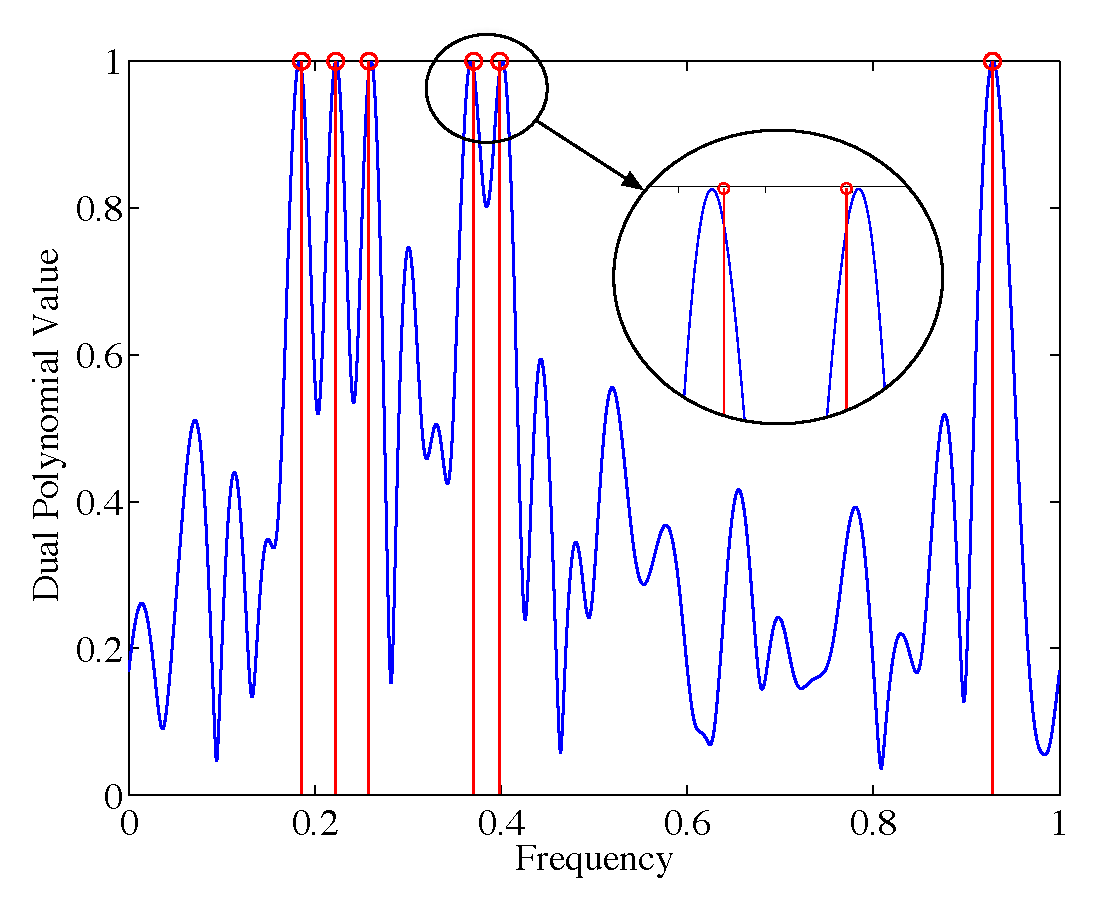
\includegraphics[width=4in]{figures/dual_poly_inset.pdf}
% \includegraphics[width=2.3in]{figures/dual_poly_inset2}
\caption{ \textbf{Frequency Localization using Dual Polynomial}: The
actual location of the frequencies in the line spectral signal $x^\star \in
\C^{64}$ is shown in red. The blue curve is the dual polynomial
obtained by solving \eqref{eq:dual-ast} with $y = x^\star + w$ where $w$ is noise of SNR 10 dB.}

\label{fig:dual_poly_localize}
\end{figure}

As shown in Corollary~\ref{cor:dual-cert-support}, the dual solution can be
used to identify the frequencies of the primal solution. For line spectra, a frequency
$f \in [0,1]$ is in the support of the solution $\hat{x}$ of \eqref{AST} if and
only if
\[
	 |\langle \hat{z}, a_{f,\phi} \rangle| =\left|\ \sum_{l=0}^{n-1} \hat{z}_l e^{-i 2\pi l f} \right| = \tau
\]
That is, $f$ is in the support of $\hat{x}$ if and only if it is a point of maximum modulus for the dual polynomial. Thus, the support
may be determined by finding frequencies $f$ where the dual polynomial attains magnitude $\tau$. 

Figure~\ref{fig:dual_poly_localize} shows the dual
polynomial for $\eqref{AST}$ with $n = 64$ samples and $k = 6$
 randomly chosen frequencies. The regularization
parameter $\tau$ is chosen as described in Section \ref{subsec:parameter}.

A recent result by Candes and Fernandez-Granda~\cite{CandesGranda} establishes
that in the noiseless case, the frequencies localized by the dual polynomial
are exact provided the minimum separation between the frequencies is at least
$4/n$ where $n$ is the number of samples in the line spectral signal. Under similar separation condition, numerical simulations suggest that \eqref{AST} achieves approximate frequency location in the noisy case. 

\section{Related Work}
\label{sec:prony-method}

% \todo{Reduce Prony}
% \todo{Prony, Music, Cadzow, Matrix Pencil only 1 para}
% \todo{Discretization Malioutov and Basis Mismatch}
% \todo{Candes}

% This
% technique is attributed to Prony in the eighteenth century.

The classical methods of line spectral estimation, often called linear
prediction methods, are built upon the seminal interpolation method of
Prony~\cite{prony1795}. In the noiseless case, with as little as $n=2k$
measurements, Prony's technique can identify the frequencies exactly, no matter
how close the frequencies are. However, Prony's technique is known to be
sensitive to noise due to instability of polynomial rooting~\cite{kahn92}.
Following Prony, several methods have been employed to robustify polynomial
rooting method including the Matrix Pencil algorithm~\cite{hua02}, which
recasts the polynomial rooting as a generalized eigenvalue problem and cleverly
uses extra observations to guard against noise. The MUSIC~\cite{music} and
ESPRIT~\cite{esprit} algorithms exploit the low rank structure of the
autocorrelation matrix.


Cadzow~\cite{cadzow02} proposed a heuristic that improves over MUSIC by 
exploiting the Toeplitz structure of the matric of moments by alternately
projecting between the linear space of Toeplitz matrices and the space of rank
$k$ matrices where $k$ is the desired model order.
Cadzow's technique is very similar~\cite{ssa_special_issue} to a popular
technique in time series literature~\cite{tsbook1,tsbook2} called Singular
Spectrum Analysis~\cite{ssa}, which uses autocorrelation matrix instead
of the matrix of moments for projection. Both these techniques may be viewed as
instances of structured low rank approximation~\cite{chu2003structured} which
exploit additional structure beyond low rank structure used in subspace based
methods such as MUSIC and ESPRIT. Cadzow's method has been identified as a  fruitful preprocessing step for linear prediction methods~\cite{blu08}. A  survey of classical linear prediction methods can be found in~\cite{blu08,StoicaMoses} and an extensive list of references is given in~\cite{stoica93}.

Most, if not all of the linear prediction methods need to estimate the model
order by employing some heuristic and the performance of the algorithm is
sensitive to the model order. In contrast, our algorithms AST and the Lasso
based method, only need a rough estimate of the noise variance. In our experiments, we provide
the true model order to Matrix Pencil, MUSIC and Cadzow methods, while we use
the estimate of noise variance for AST and Lasso methods, and still compare favorably to the classical line spectral methods.

In contrast to linear prediction methods, a number of authors
~\cite{chen98spectrum,malioutov05,bourguignon2007irregular}
have suggested using compressive sensing and viewing the frequency estimation
as a sparse approximation problem. For instance,~\cite{malioutov05} notes that
the Lasso based method has better empirical localization performance than the
popular MUSIC algorithm. However, the theoretical analysis of this phenomenon
is complicated because of the need to replace the continuous frequency space by
an oversampled frequency grid. Compressive sensing based results (see, for
instance,~\cite{duartescs}) need to carefully control the incoherence of their
linear maps to apply off-the-shelf tools from compressed sensing. It is
important to note that the performance of our algorithm improves as the grid
size increases. But this seems to contradict conventional wisdom in compressed
sensing because our design matrix $\Phi$ becomes more and more coherent, and
limits how fine we can grid for the theoretical guarantees to hold.

We circumvent the problems in the conventional compresssive sensing analysis by
directly working in the continuous parameter space and hence step away from
such notions as coherence, focussing on the geometry of the atomic set as the
critical feature. By showing that the continuous approach is the limiting
case of  the Lasso based methods using the convergence of the corresponding
atomic norms, we justify denoising line spectral signals using Lasso on a
large grid. Since the original submission of this manuscript,
Cand\`es and Fernandez-Granda~\cite{CandesGranda} showed that our SDP
formulation exactly recovers the correct frequencies in the noiseless case.

To date, line spectral analysis may be broadly classified into two camps.
\emph{Subspace methods}~\cite{music,esprit,cadzow05,ssa} build upon polynomial
interpolation~\cite{prony1795} and exploit certain low rank structure in the
spectrum estimation problem for denoising. Research on subspace approaches has
yielded several standard algorithms that are widely deployed and shown to
achieve Cram\'{e}r-Rao bound asymptotically~\cite{fri,cramer-subspace}.
However, the sensitivity to noise and model order is not well understood, and
there are few guarantees of how these algorithms perform given a limited number
of noisy measurements. For a review of many of these classical approaches, see
for example~\cite{StoicaMoses}.

More recently, approaches based on convex optimization have gained favor and
have been demonstrated to perform well on a variety of spectrum estimation
tasks~\cite{malioutov05,bourguignon2007irregular,baraniuk2010model,zweig2003irregular}. These convex programming methods restrict the frequencies to lie on a
finite grid of points and view line spectral signals as a sparse combination of
single frequencies. While these methods are reported to have significantly
better localization properties than subspace methods (see for
example,~\cite{malioutov05}) and admit fast and robust algorithms, they have
two significant drawbacks. First, while finer gridding may lead to better
performance, very fine grids are often numerically unstable. Furthermore,
traditional compressed sensing theory does not adequately characterize the
performance of fine gridding in these algorithms as the dictionary becomes
highly coherent.

Some very recent work~\cite{btr12,cg_exact12,cg_noisy} bridges the gap between
the performant discretized algorithms and continuous subspace approaches by
developing a new theory of convex relaxations for infinite continuous
dictionary of frequencies. Our work in~\cite{btr12} applies the atomic norm
framework proposed by Chandrasekaran et al~\cite{crpw} to the line spectral
estimation problem. There, we established stability results on the denoising
error and demonstrated empirically that our algorithm compared favorably with
both the classical and recent convex approaches which assume the frequencies
are on an oversampled DFT grid. Our prior results made no assumption about the
separation between frequencies. When the frequencies are well separated, the
current work demonstrates that much faster convergence rates are achieved.

Our work is closely related to recent results established by Cand\`es and
Fernandez-Granda~\cite{cg_exact12} on exact recovery using convex methods and
their recent work~\cite{cg_noisy} on exploiting the robustness of their dual
polynomial construction to show super-resolution properties of convex methods.
The total variation norm formulation used in~\cite{cg_noisy} is equivalent to
the atomic norm specialized to the line spectral estimation problem.

Robustness bounds were established in both our earlier work~\cite{btr12} and in
the work of Cand\`es and Fernandez-Granda~\cite{cg_noisy}. In~\cite{btr12}, a
slow convergence rate was established with no assumptions about the separation
of frequencies in the true signal. In~\cite{cg_noisy}, the authors provide
guarantees on the $L_1$ energy of error in the frequency domain in the case
that the frequencies are well separated. The noise is assumed to be adversarial
with a small $L_1$ spectral energy. In contrast, our paper shows near minimax
denoising error under Gaussian noise. It is also not clear that there is a
computable formulation for the optimization problem analyzed
in~\cite{cg_noisy}. While the guarantees the authors derive in~\cite{cg_noisy}
are not comparable with our results, several of their mathematical
constructions are used in our proofs here.

Additional recent work derives conditions for approximate support recovery
under the Gaussian noise model using the Beurling-Lasso ~\cite{azais}. There,
the authors show that there is a true frequency in the neighborhood of every
estimated frequency with large enough amplitude. We note that the
Beurling-Lasso is equivalent to the atomic norm algorithm that we analyze in
this paper. A more recent paper by Fernandez-Granda{\cite{granda2}} improves
this result by giving conditions on recoverability in terms of the true signal
instead of the estimated signal and prove a theorem similar to
Theorem~\ref{support}, but use a worst case $L_2$ bound on the noise samples.
Here, we improve these recent results in our proof of Theorem~\ref{support},
providing tighter guarantees under the Gaussian noise model.
 
\section{What is the best rate we can expect?}\label{sec:minimax}

Using results about minimax achievable rates for linear models~
\cite{cd_minimax,rw_minimax}, we can deduce that the convergence rate stated in
\eqref{fast-rate} is near optimal. Define the set of $k$ well separated
frequencies as

\[
\mathcal{S}_k = \left\{(f_1, \dots, f_k) \in \mathbb{T}^k ~\middle|~  d(f_p, f_q) \geq 4/n, p \neq q \right\}
\]

The expected minimax denoising error $M_k$ for a line spectral signal with
frequencies from $\mathcal{S}_k$ is defined as the lowest expected denoising
error rate for any estimate $\hat{x}(y)$ for the worst case signal $x^\star$
with support $T(x^\star) \in \mathcal{S}_k$. Note that we can lower bound $M_k$
by restricting the set of candidate frequencies to smaller set. To that end,
suppose we restrict the signal $x^\star$ to have frequencies only drawn from an
equispaced grid on the torus $T_n := \{ 4 j/n \}_{j=1}^{n/4}$. Note that any set
of $k$ frequencies from $T_n$ are pairwise separated by at least $4/n$. If we
denote by $F_n$ a $n \times (n/4)$ partial DFT matrix with (unnormalized)
columns corresponding to frequencies from $T_n$, we can write $x^\star = F_n
c^\star$ for some $c^\star$ with $\vnorm{c^\star}_0 = k$. Thus,

\begin{align*}
M_k &:= \inf_{\hat{x}}
 \sup_{
	T(x^\star) \in \mathcal{S}_k}
\frac{1}{n} \mathbb{E} \vnorm{\hat{x} - x^\star}_2^2
	\\
&\geq \inf_{\hat{x}} 
 \sup_{
	\vnorm{c^\star}_0 \leq k
	} \frac{1}{n} \mathbb{E} \vnorm{\hat{x} - F_n c^\star}_2^2\\
&\geq \inf_{\hat{c}}
 \sup_{\vnorm{c^\star}_0 \leq k} \frac{1}{n} \mathbb{E} \vnorm{F_n(\hat{c} - c^\star)}_2^2\\
&\geq  \frac{n}{4} \left\{ \inf_{\hat{c}}
 \sup_{\vnorm{c^\star}_0 \leq k}\frac{4}{n} \mathbb{E} \vnorm{\hat{c} - c^\star}_2^2\right\}\,.
\end{align*}

Here, the first inequality is the restriction of $T(x^\star)$. The second
inequality follows because we project out all components of $\hat{x}$ that do
not lie in the span of $F_n$. Such projections can only reduce the Euclidean
norm. The third inequality uses the fact that the minimum singular value of
$F_n$ is $n$ since $F_n^*F_n = n I_{{n}/{4}}$. Now we may directly apply the
lower bound for estimation error for linear models derived by Cand\'es and
Davenport. Namely, Theorem 1 of~\cite{cd_minimax} states that

\begin{align*}
\inf_{\hat{c}}
 \sup_{\vnorm{c^\star}_0 \leq k} \frac{4}{n} \mathbb{E} \vnorm{\hat{c} - c^\star}_2^2&\geq {C} \sigma^2 \frac{k \log\left(\frac{n}{4k}\right)}{\vnorm{F_n}_\mathrm{F}^2}\,.
 \end{align*} With the preceding analysis and the fact that $\vnorm{F_n}_{\mathrm{F}}^2 = n^2/4$, we can thus deduce the following theorem:
 \begin{theorem}
\label{minimax}
Let $x^\star$ be a line spectral signal as described by \eqref{eq:signal} with the support $T(x^\star) = \{f_1, \dots, f_k\} \in \mathcal{S}_k$ and $y = x^\star + w$, where $w \in \C^n$ is circularly symmetric Gaussian noise with variance $\sigma^2 I_n$. Let $\hat{x}$ be any estimate of $x^\star$ using $y$. Then,
\[
M_k = \inf_{\hat{x}}
 \sup_{
	T(x^\star) \in \mathcal{S}_k}
\frac{1}{n} \mathbb{E} \vnorm{\hat{x} - x^\star}_2^2
\geq C\sigma^2 \frac{k \log\left(\frac{n}{4k}\right)}{n}
\]
for some constant $C$ that is independent of $k$, $n$, and $\sigma$.
\end{theorem}

This theorem and Theorem~\ref{main} certify that AST is nearly minimax optimal for spectral estimation of well separated frequencies. 



\section{Proofs of Main Theorems}
\label{sec:proofs}

In this section, there are many numerical constants.  Unless otherwise specified, $C$ will denote a numerical constant whose value may change from equation to equation.  Specific constants will be highlighted by accents or subscripts.

We describe the preliminaries and notations, and restate some recent results we used 
before sketching the proof of Theorems \ref{main} and \ref{support}.

\subsection{Preliminaries}
The sample $x^\star_j$ may be regarded as the $j$th trigonometric moment of 
the discrete measure $\mu$ given by \eqref{mu}:
\begin{eqnarray*}
  x_j^\star & = & \int_0^1 e^{i 2 \pi j f} \mu ( d f)
\end{eqnarray*}
for $-m \leq j \leq m$.
Thus, the problem of extracting the frequencies and amplitudes from noisy 
observations may be regarded as the inverse problem of estimating a measure 
from noisy trigonometric moments.

We can write the vector $x^\star$ of observations $[x_{-m}^\star, \ldots, x_m^\star]^T$ in terms of an \emph{atomic decomposition}
\[
x^\star = \sum_{l=1}^k c_l a(f_l)
\]
or equivalently in terms of a corresponding \emph{representing measure} $\mu$ given by \eqref{mu} satisfying
\[
x^\star = \int_0^1 a(f) \mu(df)
\]
There is a one-one correspondence between atomic decompositions and representing measures. Note that there are infinite atomic decompositions of $x^\star$ and also infinite corresponding representing measures. However, since every collection of $n$ atoms is linearly independent, $\A$ forms a full spark frame~\cite{spark} and therefore the problem of finding the sparsest decomposition of $x^\star$ is well-posed if there is a decomposition which is at least $n/2$ sparse.

The atomic norm of a vector $z$ defined in \eqref{def-atnorm} is the minimum total variation norm~\cite{cs_otg,tvnorm} $\vnorm{\mu}_{\mathrm{TV}}$ of all representing measures $\mu$ of $z$. So, minimizing the total variation norm is the same as finding a decomposition that achieves the atomic norm.

\subsection{Dual Certificate and Exact Recovery}

Atomic norm minimization attempts to recover the sparsest  decomposition by finding a decomposition that achieves the atomic norm, i.e., find ${c_l,f_l}$ such that  $x^\star = \sum_l c_l a(f_l)$ and $
\vnorm{x^\star}_\A = \sum_l |c_l| 
$ or equivalently, finding a representing measure $\mu$ of the form \eqref{mu} that minimizes the total variation norm $
\vnorm{\mu}_{\mathrm{TV}}$. The authors  of~\cite{cg_exact12} showed 
that when $n > 256$, the  decomposition that achieves the atomic norm is the sparsest decomposition 
by explicitly constructing a dual certificate~\cite{dualcert} of optimality, whenever the composing 
frequencies $f_1, \ldots, f_k$ satisfy a minimum separation condition~\eqref{min-sep}. In the rest of the paper, we always make the technical assumption that $n > 256$.

\begin{definition}[Dual Certificate]
\label{dual-cert}
A vector $q \in \C^n$ is called a dual certificate for $x^\star$ if for the corresponding trigonometric polynomial $Q(f) := \langle q, a(f) \rangle$, we have
$$Q(f_l) = \operatorname{sign}(c_l), l = 1, \ldots, k$$  and $$|Q(f)| < 1$$ whenever $f\not\in \{ f_1, \ldots, f_k\}$.
\end{definition}
The authors of ~\cite{cg_exact12} not only explicitly constructed 
such a certificate characterized by the dual polynomial $Q$, but also showed that their construction satisfies some stability conditions, which is crucial for showing that denoising using the atomic norm provides stable recovery in the presence of noise.

\begin{theorem}[Dual Polynomial Stability, Lemma 2.4 and 2.5 in \cite{cg_noisy}]
\label{dual-stab} For any $f_1, \ldots, f_k$ satisfying the separation condition \eqref{min-sep} and any sign vector $v \in \C^k$ with $|v_j|=1$, there exists a trigonometric polynomial $Q = \left<q, a(f)\right>$ for some $q \in \C^n$ with the following properties: 
\begin{enumerate}
\item For each $j = 1, \ldots, k$, $Q$ interpolates the sign vector $v$ so that $Q(f_j) = v_j$
\item In each neighborhood $N_j$ corresponding to $f_j$ defined by
$N_j = \left\{ f : d(f, f_j) < {0.16}/{n} \right\}$, 
the polynomial $Q(f)$ behaves like a quadratic and there exist constants $C_a, C_a'$ so that
\begin{align}
\label{q1}|Q(f)| & \leq 1 - \frac{C_a}{2} n^2 (f-f_j)^2\\
\label{q2}|Q(f) - v_j| & \leq \frac{C_a'}{2} n^2 (f - f_j)^2
\end{align}
\item When $f \in F = [0,1] \backslash \cup_{j=1}^k{N_j}$, there is a numerical constant $C_b>0$ such that
\[
|Q(f)| \leq 1 - C_b
\]
\end{enumerate}
\end{theorem}

We use results in~\cite{cg_noisy} and~\cite{btr12} (reproduced in Appendix D for convenience) and borrow several ideas from the proofs in~\cite{cg_noisy}, with nontrivial modifications to establish the error rate of atomic norm regularization.

\subsection{Proof of Theorem~\ref{main}}
Let $\hat{\mu}$ be the representing measure for the solution $\hat{x}$  of \eqref{atnorm-denoise} with minimum total variation norm, that is,
\[
\hat{x} = \int_0^1 a(f) \hat{\mu}(df)
\]
and $\vnorm{\hat{x}}_\A = \vnorm{\hat{\mu}}_{\mathrm{TV}}$. Denote the error vector by $e = x^\star - \hat{x}$. 
Then, the difference measure $\nu = \mu - \hat{\mu}$ is a representing measure for $e$. We first express the denoising error $\vnorm{e}_2^2$ as the integral of the error function $E(f) = \langle e, a(f) \rangle,$ against the difference measure $\nu$:
\begin{align*}
\vnorm{e}_2^2 &= \langle e, e \rangle\\
& = \left\langle e, \int_0^1 a(f) \nu(df) \right\rangle\\
& =  \int_0^1  \left\langle e,a(f) \right\rangle \nu(df)\\
& = \int_0^1 E(f) \nu(df).
\end{align*}


Using a Taylor series approximation in each of 
the near regions $N_j$, we first show that the denoising error (or in general any 
integral of a trigonometric polynomial against the difference measure) can be controlled in terms 
of an integral in the far region $F$ and the zeroth, first, and second 
moments of the difference measure in the near regions.  The precise result is presented in the following lemma, whose proof is given in Appendix \ref{apx:pf:taylor}.
\begin{lemma}
\label{part1}
Define
\begin{align*} 
I_0^j &:= \left| \int_{N_j} \nu(df) \right|\\
I_1^j &:= n \left| \int_{N_j} (f-f_j) \nu(df) \right|\\
I_2^j &:= \frac{n^2}{2} \int_{N_j} (f-f_j)^2 |\nu|(df)\\
I_l &:= \sum_{j=1}^k I_l^j,~~\mbox{for}~l = 0, 1, 2\,.
\end{align*}
Then for any $m$th order trigonometric polynomial $X$, we have
\[
\int_0^1{ X(f) \nu(df)}
\leq \vnorm{X(f)}_\infty \left(\int_F{|\nu|(df)} + I_0 + I_1 + I_2\right)
\]
\end{lemma}

Applying Lemma \ref{part1} to the error function, we get
\begin{equation}
\label{ebd}
\vnorm{e}_2^2 \leq \vnorm{E(f)}_\infty 
\left( \int_F{|\nu|(df)} + I_0 + I_1 + I_2\right)
\end{equation}
As a consequence of our choice of $\tau$ in \eqref{tau}, we can show that $\vnorm{E(f)}_\infty \leq (1+2\eta^{-1})\tau$ with high probability. In fact, we have
\begin{align*}
\vnorm{E(f)}_\infty &= \sup_{f \in [0,1]}\left|\langle e, a(f) \rangle\right|\\
&= \sup_{f \in [0,1]} \left| \langle x^\star - \hat{x}, a(f) \rangle\right|\\
&\leq \sup_{f \in [0,1]} \left| \langle w, a(f) \rangle \right| +  \sup_{f \in [0,1]} \left| \langle y - \hat{x}, a(f) \rangle \right|\\
&\leq \sup_{f \in [0,1]} \left| \langle w, a(f) \rangle \right| +  \tau\\
\label{errbd} \numberthis &\leq (1 +2\eta^{-1})\tau \leq 3 \tau, \text{with high probability.}
\end{align*}
The second inequality follows from the optimality conditions for \eqref{atnorm-denoise}. It is shown in Appendix C of ~\cite{btr12} that the penultimate inequality holds with high probability.

Therefore, to complete the proof, it suffices to show that the other terms on the right hand side of \eqref{ebd} are $O(\frac{k\tau}{n})$.  While there is no exact frequency recovery in the presence of noise, we can hope to get the frequencies approximately right. Hence, we expect that the integral in the far region can be well controlled and the local integrals of the difference measure in the near regions are also small due to cancellations. Next, we utilize the properties of the dual polynomial in Theorems~\ref{dual-stab} and another polynomial given in Theorem~\ref{dual-lin}  in Appendix \ref{apx:collection} to show that the zeroth and first moments of $\nu$ may be controlled in terms of the other two quantities in \eqref{ebd} to upper bound the error rate. The following lemma is similar to Lemmas 2.2 and 2.3 in~\cite{cg_noisy}, but we have made several modifications to adapt it to our signal and noise model. For completeness, we provide the proof in Appendix \ref{apx:pf:I0I1}. 

\begin{lemma}
\label{part2}
There exists numeric constants $C_0$ and $C_1$ such that
\begin{align*}
I_0 &\leq C_0 \left(\frac{k \tau}{n} + I_2 + \int_F{|\nu|(df)}\right) \\
I_1 &\leq C_1 \left(\frac{k \tau}{n} + I_2 + \int_F{|\nu|(df)}\right).
\end{align*}
\end{lemma}

All that remains to complete the proof is an upper bound on $I_2$ and $\int_F{|\nu|(df)}$.  The key idea in establishing such a bound is deriving upper and lower bounds on the
difference $\| P_{T^c} ( \nu) \|_{{\mathrm{TV}}} - \| P_T ( \nu) \|_{{\mathrm{TV}}}$
between the total variation norms of $\nu$ on and off the support. The upper bound can be derived using optimality conditions. We lower bound $\| P_{T^c} ( \nu)
\|_{{\mathrm{TV}}} - \| P_{T} ( \nu) \|_{{\mathrm{TV}}}$ using the fact that a constructed dual
certificate $Q$ has unit magnitude for every element in the support
$T$ of $P_T ( \nu)$ whence we have $\| P_T ( \nu) \|_{{\mathrm{TV}}} = \int_{\mathbb{T}}
Q ( f) \nu ( d f)$. A critical element in deriving both the lower and upper bounds is that the dual polynomial $Q$ has quadratic drop in each near regions $N_j$ and is bounded away from one in the far region $F$. Finally, by combing these bounds and carefully controlling the regularization parameter, we get the desired result summarized in the following lemma. The details of the proof are fairly technical and we leave them to Appendix \ref{apx:pf:I2far}.

\begin{lemma}
Let $\tau = \eta\sigma \sqrt{n\log(n)}$. If $\eta>1$ is large enough, then there exists a numerical constant $C$ such that, with high probability
\label{part3}
\[
\int_F{|\nu|(df)} + I_2 \leq \frac{C k \tau}{n}.
\]
\end{lemma}

Putting together Lemmas \ref{part1}, \ref{part2} and \ref{part3}, we finally prove our main theorem:
\begin{align*}
\frac{1}{n}\vnorm{e}_2^2 
&\leq \frac{\vnorm{E(f)}_\infty}{n} \left(\int_F{|\nu|(df)} + I_0 + I_1 + I_2\right)\\
&\leq \frac{\vnorm{E(f)}_\infty}{n} \left(\frac{C_1 k \tau}{n} + C_2 \int_F{|\nu|(df)} + C_3 I_2\right)\\
&\leq  \frac{\vnorm{E(f)}_\infty}{n} \frac{C k \tau}{n} \\
& \leq \frac{C k \tau^2}{n^2}\\
&= O\left(\sigma^2\frac{k \log(n)}{n}\right).
\end{align*}
The first three inequalities come from successive applications of Lemmas 1, 2 and 3 respectively. The fourth inequality follows from \eqref{errbd} and the fifth by our choice of $\tau$ according to Eq. \eqref{tau}. This completes the proof of Theorem \ref{main}.



\subsection{Proof of Theorem~\ref{support}}
\label{sec:support}
The first two statements in Theorem \ref{support} are direct consequences of Lemma~\ref{part3}. For (iii.), we follow~\cite{granda2} and  use the dual polynomial $Q_j^{\star} ( f) = \langle q_j^{\star}, a ( f)\rangle$ constructed in Lemma 2.2 of~\cite{granda2} which satisfies
\begin{eqnarray*}
  Q_j^{\star} ( f_j) & = & 1\\
  | 1 - Q_j^{\star} ( f) | & \leq & n^2 C_1' ( f - f_j)^2, f \in N_j\\
  | Q_j^{\star} ( f) | & \leq & n^2 C_1' ( f - f_{j'})^2, f \in N_{j'}, j' \neq
  j\\
  | Q_j^{\star} ( f) | & \leq & C_2', f \in F.
\end{eqnarray*}
We note that $c_j - \sum_{\hat{f}_l \in N_j} \hat{c}_l = \int_{N_j} \nu(df)$. Then, by applying triangle inequality several times,
\begin{align*}
\left| \int_{N_j}  \nu(df)\right|
& \leq \left| \int_{N_j}  Q_j^\star (f) \nu(df)\right| + \left| \int_{N_j}  (1-Q_j^\star (f)) \nu(df)\right|\\
& \leq \left| \int_0^1  Q_j^\star (f) \nu(df)\right| + \left| \int_{N_j^c}  Q_j^\star (f) \nu(df)\right| + \left| \int_{N_j}  (1-Q_j^\star (f)) \nu(df)\right|\\
& \leq \left|\int_0^1  Q_j^\star (f) \nu(df)\right| + \left| \int_{F}  Q_j^\star (f) \nu(df)\right| \\
&\qquad\qquad\qquad + \sum_{\substack{j' \neq j\\j'=1}}^k \int_{N_{j'}} \left| Q_j^\star (f)\right| |\nu|(df) +  \int_{N_j}  \left|1-Q_j^\star (f)\right| |\nu(df)|\,.
\end{align*}

We upper bound the first term using Lemma~\ref{l4} in Appendix \ref{apx:collection} which yields
\[
\left| \int^0_{1}  Q_j^\star (f) \nu(df)\right| \leq \frac{Ck \tau}{n}
\]
The other terms can be controlled using the properties of $Q_j^\star$:
\begin{align*}
\left| \int_{F}  Q_j^\star (f) \nu(df)\right| & \leq C_2' \int_{F} |\nu| (df)\\
\sum_{\substack{j' \neq j\\j'=1}}^k \int_{N_{j'}} \left| Q_j^\star (f)\right| |\nu|(df) +  \int_{N_j}  \left|1-Q_j^\star (f)\right| |\nu|(df)
& \leq
 C_1'\sum_{j'=1}^k \int_{N_{j'}} n^2 (f-f_{j'})^2 |\nu|(df) = C_1 I_2
\end{align*}
Using Lemma~\ref{part3}, both of the above are upper bounded by $\frac{C k \tau}{n}$. Now, by combining these upper bounds, we finally have
\[
\left| c_j - \sum_{l : \hat{f}_l \in N_j} \hat{c}_l \right| \leq \frac{C_3 k \tau}{n}
\]
This shows part (iii) of the theorem. Part (iv) can be obtained by combining parts (ii) and (iii).

\section{Unsorted Appendices}
\subsection{Proof of Lemma \ref{part1}}\label{apx:pf:taylor}
We first split the domain of integration into the near and far regions.
\begin{align}
\left |\int_0^1 X(f) \nu(df)\right | 
&\leq \left |\int_F X(f) \nu (f)\right | + \sum_{j=1}^k \left | \int_{N_j}X(f) \nu(df)\right |\nonumber \\
&\leq \vnorm{X(f)}_\infty \int_F |\nu| (df) + \sum_{j=1}^k \left | \int_{N_j}X(f) \nu(df) \right |.\label{Xfbd}
\end{align}
by using H\"{o}lder's inequality for the last inequality. Using Taylor's theorem, we may expand the integrand $X(f)$ around $f_j$ as
\[
X(f) = X(f_j) + (f-f_j) X'(f_j) + \frac{1}{2} X''(\xi_j) (f-f_j)^2 
\]
for some $\xi_j \in N_j$. 
Thus,
{\small
\begin{align*}
&|X(f)-X(f_j)-X'(f_j)(f-f_j)|\\
&\leq \sup_{\xi \in N_j} \frac{1}{2}|X''(\xi)|(f -f_j)^2\\ &\leq \frac{1}{2} n^2 \vnorm{X(f)}_\infty(f - f_j)^2, 
\end{align*}
}
where for the last inequality we have used a theorem of Bernstein for trigonometric polynomials (see, for example~\cite{bernstein}):  
\begin{align*}
|X'(f_j)|  & \leq n \vnorm{X(f)}_\infty\\
|X''(f_j)| & \leq n^2 \vnorm{X(f)}_\infty.
\end{align*}
As a consequence, we have
\begin{align*}
\left | \int_{N_j} X(f) \nu(df)\right| &\leq \left| X(f_j)\right| \left| \int_{N_j} \nu (df)\right| + \left|X'(f_j)\right| \left|\int_{N_j} (f-f_j) \nu (df)  \right|\\
& + \frac{1}{2} n^2 \|X(f)\|_\infty \int_{N_j} (f-f_j)^2 |\nu| (df) \\
& \leq \|X(f)\|_\infty \left(I_0^j + I_1^j + I_2^j\right).
\end{align*}
Substituting back into \eqref{Xfbd} yields the desired result.

\subsection{Some useful lemmas}
\label{apx:collection}
In addition to Theorem~\ref{dual-stab}, we recall another result in~\cite{cg_noisy} where the authors show the existence of a 
trigonometric polynomial $Q_1$ that is linear in each $N_j$ which is also an essential ingredient in our proof.

\begin{theorem}[Lemma 2.7 in~\cite{cg_noisy}]
\label{dual-lin}
For any $f_1, \ldots, f_k$ satisfying \eqref{min-sep} and any sign vector $v \in \C^k$ with $|v_j|=1$, there exists a polynomial $Q_1 = \left<q_1, a(f)\right>$ for some $q_1 \in \C^n$ with the following properties: 
\begin{enumerate}
\item For every $f \in N_j,$ there exists a numerical constant $C_a^1$ such that
\begin{equation}
\label{ca1}
|Q_1(f) - v_j(f-f_j)| \leq \frac{n}{2} C_a^1 (f-f_j)^2
\end{equation}
\item For $f \in F$, there exists a numerical constant $C_b^1$ such that
\begin{equation}
\label{cb1}
|Q_1(f)| \leq \frac{C_b^1}{n}.
\end{equation}
\end{enumerate}
\end{theorem}

We will also need the following straightforward consequence of the constructions of the polynomials in Theorem \ref{dual-stab}, Theorem \ref{dual-lin}, and Section \ref{sec:support}.
\begin{lemma}
\label{l1}
There exists a numerical constant $C$ such that the constructed $Q(f)$ in Theorem \ref{dual-stab}, $Q_1(f)$ in Theorem \ref{dual-lin}, and $Q_j^\star(f)$ in Section \ref{sec:support} satisfy respectively
\begin{align}
\|Q(f)\|_1 &:= \int_0^1{| Q(f)| df} \leq \frac{C k}{n}\label{QL1}\\
\| Q_1(f)\|_1 &\leq \frac{C k}{n^2}\label{Q1L1}\\
\|Q_j^\star\|_1 & \leq \frac{Ck}{n}\label{QjL1}.
\end{align}
\end{lemma}
\begin{proof}
We will give a detailed proof of \eqref{QL1}, and list the necessary modifications for proving \eqref{Q1L1} and \eqref{QjL1}. The dual polynomial $Q(f)$ constructed in \cite{cg_exact12} is of the
form
\begin{eqnarray}
  Q \left( f \right) & = & \sum_{f_j \in T} \alpha_j K \left( f - f_j \right)
  + \sum_{f_j \in T} \beta_j K' \left( f - f_j \right) \label{formofQ}
\end{eqnarray}
where $K \left( f \right)$ is the squared Fej\'er kernel (recall that $m = (n-1)/2$)
\begin{eqnarray*}
  K \left( f \right) & = & \left( \frac{\sin \left( \left( \frac{m}{2} + 1
  \right) \pi f \right)}{\left( \frac{m}{2} + 1 \right) \sin \left( \pi f
  \right)} \right)^4
\end{eqnarray*}
 and for $n \geq 257$, the coefficients
$\alpha \in \C^k$ and $\beta \in \C^k$ satisfy \cite[Lemma 2.2]{cg_exact12}
\begin{eqnarray*}
  \left\| \alpha \right\|_{\infty} & \leq & C_\alpha\\
  \left\| \beta \right\|_{\infty} & \leq & \frac{C_\beta}{n} 
\end{eqnarray*}
for some numerical constants $C_\alpha$ and $C_\beta$. 
Using \eqref{formofQ} and triangle inequality, we bound $\|Q(f)\|_1$ as follows: 
\begin{eqnarray}
  \|Q(f)\|_1 &=& \int_0^1 \left| Q \left( f \right) \right| d f\nonumber\\
  &\leq & k \left\| \alpha \right\|_\infty \int_0^1 \left| K \left( f\right) \right| d f + k \left\| \beta \right\|_\infty \int_0^1 \left| K' \left( f\right) \right| d f\label{Qbdgeneral1}\\
  & \leq & C_\alpha k \int_0^1 \left| K \left(f\right) \right| d f + \frac{C_\beta}{n} k \int_0^1 \left|K'(f)\right|d f \label{Q1bd},
 \end{eqnarray}
 
To continue, note that $\int_0^1 | K ( f) | d  f = \int_0^1 | G ( f) |^2 d
 f =: \|G(f)\|_2^2$ where $G ( f)$ is the Fej\'er kernel, since $K(f)$ is the squared
Fej\'er kernel. We can write
\begin{eqnarray}
  G ( f)  =  \left( \frac{\sin \left( \pi \left( \frac{m}{2} + 1 \right) f
  \right)}{\left( \frac{m}{2} + 1 \right) \sin ( \pi f)} \right)^2
   =  \sum_{l = - m / 2}^{m / 2} g_l e^{- i 2 \pi f l}\label{expressionG}
\end{eqnarray}
where $g_l = \left( \frac{m}{2} + 1 - | l | \right) / \left( \frac{m}{2} + 1
\right)^2$. Now, by using Parseval's identity, we obtain
\begin{eqnarray}
 \int_0^1 |K(f)| df & = & \int_0^1 | G ( f) |^2 d f
  =  \sum_{l = - m / 2}^{m / 2} | g_l |^2\nonumber\\
  & = & \frac{1}{\left( \frac{m}{2} + 1 \right)^4} \left( \left( \frac{m}{2}
  + 1 \right)^2 + 2 \sum_{l = 1}^{m / 2} \left( \frac{m}{2} + 1 - l \right)^2
  \right)\nonumber\\
  & = & \frac{1}{\left( \frac{m}{2} + 1 \right)^4} \left( \left( \frac{m}{2}
  + 1 \right)^2 + 2 \sum_{l = 1}^{m / 2} l^2 \right)\nonumber\\
  & \leq & \frac{C}{n}\label{bdKf}
\end{eqnarray}
for some numerical constant $C$ when $n = 2 m + 1 \geq 10$.

Now let us turn our attention to $\int_0^1 | K' (
f) | d  f$. Since $K ( f) = G ( f)^2$, we have
\begin{eqnarray}
  \int_0^1 | K' ( f) | d  f  =  2\int_0^1 | G ( f) G' ( f) | d
   f
   \leq  2\| G ( f) \|_2 \| G' ( f) \|_2\label{holder}
\end{eqnarray}
We have already established that $\| G ( f) \|_2^2 \leq C / {n}$ and we
will now show that $\| G' ( f) \|_2^2 \leq C' {n}$. Differentiating the
expression for $G(f)$ in \eqref{expressionG}, we get
\begin{eqnarray*}
  G' ( f) & = & -2 \pi i \sum_{l = - m / 2}^{m / 2} l g_l e^{- i 2 \pi f l}
\end{eqnarray*}
Therefore, by applying Parseval's identity again, we get
\begin{eqnarray*}
  \| G' ( f) \|_2^2 
  & = & 4 \pi^2 \sum_{l = - m / 2}^{m / 2} l^2 | g_l |^2\\
  & \leq &  \pi^2 m^2 \sum_{l = - m / 2}^{m / 2} | g_l |^2\\
  & \leq & C' n
\end{eqnarray*}
Plugging back into \eqref{holder} yields
\begin{align}
\int_0^1 |K'(f)| df \leq C \label{bdK1f}
\end{align}
for some constant $C$. Combining \eqref{bdK1f} and \eqref{bdKf} with \eqref{Q1bd} gives the desired result in \eqref{QL1}.



The dual polynomial $Q_1(f)$ is also of the form \eqref{formofQ} with coefficient vectors $\alpha_1$ and $\beta_1$, which satisfy \cite[Proof of Lemma 2.7]{cg_noisy}
\begin{align*}
\|\alpha_1\|_\infty \leq \frac{C_{\alpha_1}}{n},\\
\|\beta_1\|_\infty \leq \frac{C_{\beta_1}}{n^2}.
\end{align*}
Combining the above two bounds with \eqref{Qbdgeneral1}, \eqref{bdK1f} and \eqref{bdKf} gives the desired result in \eqref{Q1L1}.

The last polynomial $Q_j^\star$ also has the form \eqref{formofQ} with coefficient vectors $\alpha^\star$ and $\beta^\star$. According to \cite[Proof of Lemma 2.2]{granda2}, these coefficients satisfy
\begin{align*}
\|\alpha^\star\|_\infty \leq {C_{\alpha_\star}},\\
\|\beta_\star\|_\infty \leq \frac{C_{\beta_\star}}{n},
\end{align*}
which yields \eqref{QjL1} following the same argument leading to \eqref{QL1}. 

\end{proof}

Using Lemma \ref{l1}, we can derive the estimates we need in the following lemma.
\begin{lemma}
\label{l4}
Let $\nu = \hat{\mu} - \mu$ be the difference measure. Then, there exists numerical constant $C>0$ such that
\begin{align}
\label{qv}\left| \int_0^1 Q(f) \nu(df) \right| &\leq \frac{C k \tau}{n}\\
\label{q1v}\left| \int_0^1 Q_1(f) \nu(df) \right| &\leq \frac{C k \tau}{n^2}\\
\label{qjv} \left| \int_0^1 Q_j^\star(f) \nu(df) \right| & \leq \frac{Ck\tau}{n}.
\end{align}
\end{lemma}
\begin{proof}
Let $Q_0 = \langle q_0, a(f) \rangle $ be a general trigonometric polynomial associated with $q_0 \in \C^n$. Then,
\begin{align*}
\left|\int_0^1 Q_0(f) \nu(df) \right| 
& = \left|\int_0^1 \langle q_0 , a(f) \rangle  \nu(df) \right|\\
& = \left|\langle q_0,  \int_0^1  a(f)  \nu(df) \rangle\right|\\
& = \left|\langle q_0, e \rangle\right|\\
& = \left|\langle Q_0(f), E(f) \rangle\right|\\
& \leq \vnorm{Q_0(f)}_1 \vnorm{E(f)}_\infty\,.
\end{align*}
Here we use Parseval's identity in the second to last step and H\"{o}lder's inequality in the last inequality. Then, the result follows by using Lemma~\ref{l1} and \eqref{errbd}.
\end{proof}


We also need the following consequence of the optimality condition of AST from~\cite[Lemma 2]{btr12}:
\begin{prop}\label{pro:optimality}
\begin{align}
\tau \vnorm{\hat{x}}_\A \leq \tau \vnorm{x^\star}_\A + \langle w, \hat{x} - x^\star \rangle
\end{align}
\end{prop}

\subsection{Proof of Lemma \ref{part2}}\label{apx:pf:I0I1}
Consider the polar form
\[
  \int_{N_j} \nu ( df)  =  \left| \int_{N_j} \nu ( df) \right| e^{i \theta_j} .
\]
Set $v_j = e^{-i \theta_j}$ and let $Q(f)$ be the dual polynomial promised by Theorem \ref{dual-stab} for this $v$. Then, we have 
\begin{align*}
  \left| \int_{N_j} \nu ( d f) \right| & = 
  \int_{N_j} e^{- i \theta_j} \nu ( d f)\\
  & =  \int_{N_j} Q ( f) \nu ( d f) + 
  \int_{N_j} (e^{- i \theta_j} -  Q ( f) ) \nu ( d f)
\end{align*}
Summing over $j=1,\ldots,k$ yields

\begin{align}
\nonumber I_0 &= \sum_{j=1}^k \left| \int_{N_j} \nu(df) \right|\\
\nonumber & = \sum_{j=1}^k\int_{N_j} Q ( f) \nu ( d f) + 
\sum_{j=1}^k \int_{N_j} ( v_j - Q ( f)) \nu ( d f)\\
\nonumber & \leq \left|\int_0^1 Q(f) \nu(df) \right| + \int_F|\nu|(df) + C_a' I_2, \text{ using triangle inequality and \eqref{q2}}\\
\label{i0} & \leq \frac{C k \tau}{n} + \int_F|\nu|(df) + C_a' I_2, \text{ using \eqref{qv}}.
\end{align}
We use a similar argument for bounding $I_1$ but this time use the dual polynomial $Q_1(f)$ guaranteed by Theorem \ref{dual-lin}. Again, start with the polar form
\[
  \int_{N_j} (f - f_j) \nu ( d f)  =  \left|
  \int_{N_j} (f - f_j) \nu ( d f) \right| e^{i \theta_j} = I_1^j e^{i\theta_j}/n
\]
Set $v_j = e^{-i \theta_j}$ in Theorem \ref{dual-lin} to obtain
{
\begin{align*}
  I_1^j & = 
  n\int_{N_j} e^{- i \theta_j} ( f - f_j) \nu ( d f)\\
  & =  n \int_{N_j} (v_j (
  f - f_j) - Q_1 ( f)) \nu ( d f)  + n\int_{N_j} Q_1 ( f) \nu ( d f)
\end{align*}
}
Summing over $j=1,\ldots,k$ yields
{
\begin{align}
\nonumber I_1 &= \sum_{j=1}^k I_1^j\\
\nonumber &= n \sum_{j=1}^k \int_{N_j} (v_j (
  f - f_j) - Q_1 ( f)) \nu ( d f) + n\sum_{j=1}^k\int_{N_j} Q_1 ( f) \nu ( d f)\\
\nonumber &\leq C_a^1 I_2 + n\left|\int_0^1 Q_1(f) \nu(df)\right| +  n\left |\int_F Q_1(f) \nu(df)\right |\\
\label{i1}& \leq C_a^1 I_2 + \frac{C k \tau}{n} +  C_b^1 \int_F|\nu|(df)
\end{align}
}
For the first inequality, we have used \eqref{ca1} and triangle inequality, and for the last inequality, we have used \eqref{q1v} and \eqref{cb1}. Equations \eqref{i0} and \eqref{i1} complete the proof.


\subsection{Proof of Lemma \ref{part3}}
\label{apx:pf:I2far}
Denote by $P_T(\nu)$ the projection of the difference measure $\nu$ on the support set $T = \{f_1, \ldots, f_k\}$ of $x^\star$ so that $P_T(\nu)$ is supported on $T$. Then, setting $Q(f)$ the polynomial in Theorem \ref{dual-stab} that interpolates the sign of $P_T( \nu)$, we have
{
\begin{align*}
  \| P_T ( \nu) \|_{\mathrm{TV}} & =  \int_0^1 Q ( f) P_T ( \nu) ( d f)\\
  & \leq  \left| \int_0^1 Q ( f) \nu ( d f) \right| + \left|
  \int_{T^c} Q ( f) \nu ( d f) \right|\\
  & \leq  \frac{C k \tau}{n} + \sum_{f_j \in T} \left|
  \int_{N_j / \{ f_j \}} Q ( f) \nu ( d f) \right| + \left|
  \int_F Q ( f) \nu ( d f) \right|,
\end{align*}}
where for the first inequality we used triangle inequality and for the last inequality we used \eqref{qv}. 
The integration over $F$ is can be bounded using H\"{o}lder's inequality
\[
  \left| \int_{F} Q ( f) \nu ( d f) \right|  
  \leq  ( 1 - C_b) \int_F |\nu|(df)
\]

We continue with
{
\begin{align*}
  \left| \int_{N_j / \{ f_j \}} Q ( f) \nu ( d f) \right| 
  & \leq  \left| \int_{N_j / \{ f_j \}} | Q ( f) | | \nu | ( d f) \right|\\
  & \leq  \int_{N_j / \{ f_j \}} ( 1 - \tfrac{1}{2}n^2 C_a ( f - f_j)^2) | \nu | ( d f)\\
  & \leq \int_{N_j / \{ f_j \}} | \nu | ( d f) - C_a I_2^j.
\end{align*}
}
As a consequence, we have
{
\begin{align*}
  \nonumber \| P_T ( \nu) \|_{\mathrm{TV}} & \leq  \frac{C k \tau}{n} + \sum_{f_j
  \in T} \int_{N_j / \{ f_j \}} | \nu | ( d f) - C_a
  I_2 + ( 1 - C_b) \int_F |\nu|(df) \nonumber\\
 & \leq  \frac{C k \tau}{n} + \underbrace{\sum_{f_j
  \in T} \int_{N_j / \{ f_j \}} | \nu | ( d f) + \int_F |\nu|(df)}_{\|P_{T^c}\|_{\mathrm{TV}}} - C_a
 I_2  - C_b \int_F |\nu|(df)
\end{align*}
}
or equivalently,
\begin{align}
  \label{eqn:lower}
\|P_{T^c}(\nu) \|_{\mathrm{TV}} - \|P_T(\nu)\|_{\mathrm{TV}} \geq C_a I_2 + C_b \int_F |\nu|(df) - \frac{C k\tau}{n}.
\end{align}

Now, we appeal to Proposition \ref{pro:optimality} and obtain
\[
\vnorm{\hat{x}}_\A \leq \vnorm{x^\star}_\A - \langle w, e \rangle/\tau
\]
and thus
\begin{equation}
\label{opt-cond}
\vnorm{\hat{\mu}}_{\mathrm{TV}} \leq \vnorm{\mu}_{\mathrm{TV}} + |\langle w, e \rangle|/\tau.
\end{equation}
Using Lemma~\ref{part1},
\begin{align}
\nonumber |\langle w, e \rangle| & = |\langle w, \int_0^1 a(f) \nu(df)  |\rangle\\
& = \left|\int_0^1  \left\langle w,  a(f)  \right\rangle \nu(df)\right|\\
\nonumber & \leq \vnorm{\left\langle w,  a(f)  \right\rangle}_\infty\left(\frac{C k \tau}{n} + I_0 + I_1 + I_2\right)\\
\label{w-expand}& \leq 2\eta^{-1} \tau \left(\frac{C k \tau}{n} + I_0 + I_1 + I_2\right)\nonumber \\
 & \leq C \eta^{-1} \tau \left(\frac{k\tau}{n} + I_2 + \int_F |\nu|(df) \right)
\end{align}
with high probability, where for the penultimate inequality we used our choice of $\tau$ and $\vnorm{\left\langle w,  a(f)  \right\rangle}_\infty \leq 2\eta^{-1} \tau$ with high probability, a fact shown in Appendix C of ~\cite{btr12}. 
Substituting \eqref{w-expand} in \eqref{opt-cond}, we get
\begin{align*}
& \vnorm{\mu}_{\mathrm{TV}} + C \eta^{-1} \tau \left(\frac{k\tau}{n} + I_2 + \int_F |\nu|(df) \right)\\
& \geq \vnorm{\hat{\mu}}_{\mathrm{TV}}\\
& = \vnorm{\mu + \nu}_{\mathrm{TV}}\\
& \geq \vnorm{\mu}_{\mathrm{TV}} - \vnorm{{P_T(\nu)}}_{\mathrm{TV}} + \vnorm{{P_{T^c}(\nu)}}_{\mathrm{TV}}\end{align*}
Canceling $\|\mu\|_{\mathrm{TV}}$ yields 
\begin{align}\label{eqn:upper}
\|P_{T^c}(\nu)\|_{\mathrm{TV}} - \|P_T(\nu)\|_{\mathrm{TV}} \leq C\eta^{-1}\tau \left(\frac{k \tau}{n} + I_2 + \int_F |\nu|(df)\right)
\end{align}
As a consequence of \eqref{eqn:lower} and \eqref{eqn:upper}, we get,
\[
  C(1+\eta^{-1}) \frac{k \tau}{n} \geq  ( C_b - \eta^{-1} C)  \int_F{|\nu|(df)} + ( C_a - \eta^{-1} C)I_2
\]
whence the result follows for large enough $\eta.$

\section{Experiments}
\label{sec:experiments}

\todo{Add in Experiments from Minimax Paper}

We compared the performance of AST, the discretized Lasso approximation, the
Matrix Pencil, MUSIC and Cadzow's method, both in terms of the mean squared
estimation error as in Theorem~\ref{main} and frequency localization. For our
experiments, we generated $k$ normalized frequencies $f_1^\star, \ldots,
f_k^\star$ uniformly randomly chosen from $\left[0,1\right]$ such that every
pair of frequencies are separated by at least $1/2n$. The signal $x^\star \in
\C^n$ is generated according to \eqref{eq:signal} with $k$ random amplitudes
independently chosen from $\chi^2(1)$ distribution (squared Gaussian). All of
our sinusoids were then assigned a random phase (equivalent to multiplying
$c_k^\star$ by a random unit norm complex number). Then, the observation $y$ is
produced by adding complex white gaussian noise $w$ such that the input signal
to noise ratio (SNR) is $-10,-5,0,5,10,15$ or $20$ dB. We compare the average
MSE of the various algorithms in 20 trials for various values of number of
observations $(n = 64,128,256)$, and number of frequencies $ (k =
n/4,n/8,n/16)$.


AST needs an estimate of the noise variance $\sigma^2$ to pick the
regularization parameter according to \eq{tau}. In many situations, this
variance is not known to us \emph{a priori}. However, we can construct a
reasonable estimate for $\sigma$ when the phases are uniformly random. It is
known that the autocorrelation matrix of a line spectral signal (see, for
example Chapter 4 in \cite{StoicaMoses}) can be written as a sum of a low rank
matrix and $\sigma^2 I$ if we assume that the phases are uniformly random. Since
the empirical autocorrelation matrix concentrates around the true expectation,
we can estimate the noise variance by averaging a few smallest eigenvalues of
the empirical autocorrelation matrix. In the following experiments, we form the
empirical autocorrelation matrix using the MATLAB routine \texttt{corrmtx} using
a prediction order $m=n/3$ and averaging the lower $25\%$ of the eigenvalues. We
used this estimate in equation~\eq{tau} to determine the regularization
parameter for both our AST and Lasso experiments.

First, we implemented AST using the ADMM method described in detail in
Chapter~\ref{algos}. We used the stopping criteria described in~\cite{admm2011}
and set $\rho=2$ for all experiments. We use the dual solution $\hat{z}$ to
determine the support of the optimal solution $\hat{x}$ using the procedure
described in Section~\ref{sec:frequency-localize}. Once the frequencies
$\hat{f}_l$ are extracted, we ran the least squares problem
$\mbox{minimize}_\alpha \|U \alpha - y\|^2$ where $U_{jl} = \exp(i 2\pi j
\hat{f}_l)$ to obtain a \emph{debiased} solution. After computing the optimal
solution $\alpha_{\mathrm{opt}}$, we returned the prediction $\hat{x} =
U\alpha_{\mathrm{opt}}$.

We implemented Lasso, obtaining an estimate $\hat{x}$ of $x^\star$ from $y$ by
solving the optimization problem \eqref{epsprimal} with debiasing. We use the
algorithm described in Section \ref{sec:comp-method} with grid of $N=2^{m}$
points where $m=10,11,12,13,14$ and $15$. Because of the basis mismatch effect,
the optimal $c_{\mathrm{opt}}$ has significantly more non-zero components than
the true number of frequencies. However, we observe that the frequencies
corresponding to the non-zero components of $c_{\mathrm{opt}}$ cluster
around the true ones. We therefore extract one frequency from each cluster of
non-zero values by identifying the grid point with the maximum absolute
$c_{\mathrm{opt}}$ value and zero everything else in that cluster. We then ran
a debiasing step which solves the least squares problem $\mbox{minimize}_\beta
\|\Phi_S \beta- y\|^2$ where $\Phi_S$ is the submatrix of $\Phi$ whose columns
correspond to frequencies identified from $c_{\mathrm{opt}}$. We return the
estimate $\hat{x} = \Phi_S \beta_{\mathrm{opt}}$. We used the freely
downloadable implementation of SpaRSA to solve the Lasso problem. We used a
stopping parameter of $10^{-4}$, but otherwise used the default parameters.

We implemented Cadzow's method as described by the
pseudocode in~\cite{blu08}, the Matrix Pencil as described in~\cite{hua02} and
MUSIC~\cite{music} using the MATLAB routine \texttt{rootmusic}. All these
algorithms need an estimate of the number of sinusoids. Rather
than implementing a heuristic to estimate $k$, \emph{we fed the true $k$ to our
solvers}. This provides a huge advantage to these algorithms. Neither AST or the
Lasso based algorithm are provided the true value of $k$, and the noise 
variance $\sigma^2$ required in the regularization parameter is estimated from $y$.

Let $\{\hat{c}_l\}$ and $\{\hat{f}_l\}$ denote the amplitudes and frequencies
estimated by any of the algorithms - AST, MUSIC or Cadzow. We use the following
error metrics to characterize the frequency localization of various algorithms:
\begin{enumerate} \item[(i)] Sum of the absolute value of amplitudes in the far
region $F$, $m_1 = \sum_{l : \hat{f}_l \in F} |\hat{c}_l|$ \item[(ii)] The
weighted frequency localization error, $m_2 = \sum_{l : \hat{f}_l \in N_j}
|\hat{c}_l| \{ \min_{f_j \in T} d(f_j,\hat{f}_l) \}^2$ \item[(iii)] Error in
approximation of amplitudes in the near region, $m_3 = \left| c_j - \sum_{l :
\hat{f_l} \in N_j} \hat{c}_l \right|$ \end{enumerate} These are precisely the
quantities that we prove tend to zero in Theorem~\ref{support}.

\begin{figure*}[htbp]
  \begin{tabular}{c}
	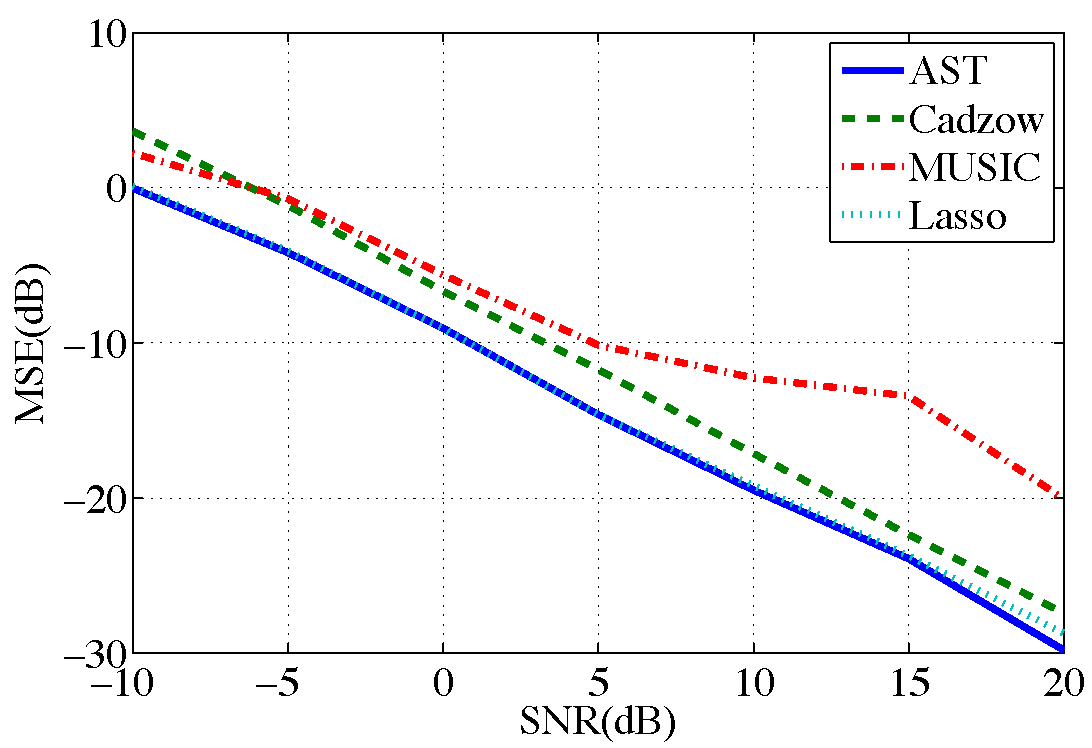
\includegraphics[width=0.5\textwidth]{figures/mse_snr_128_8_randamp}
	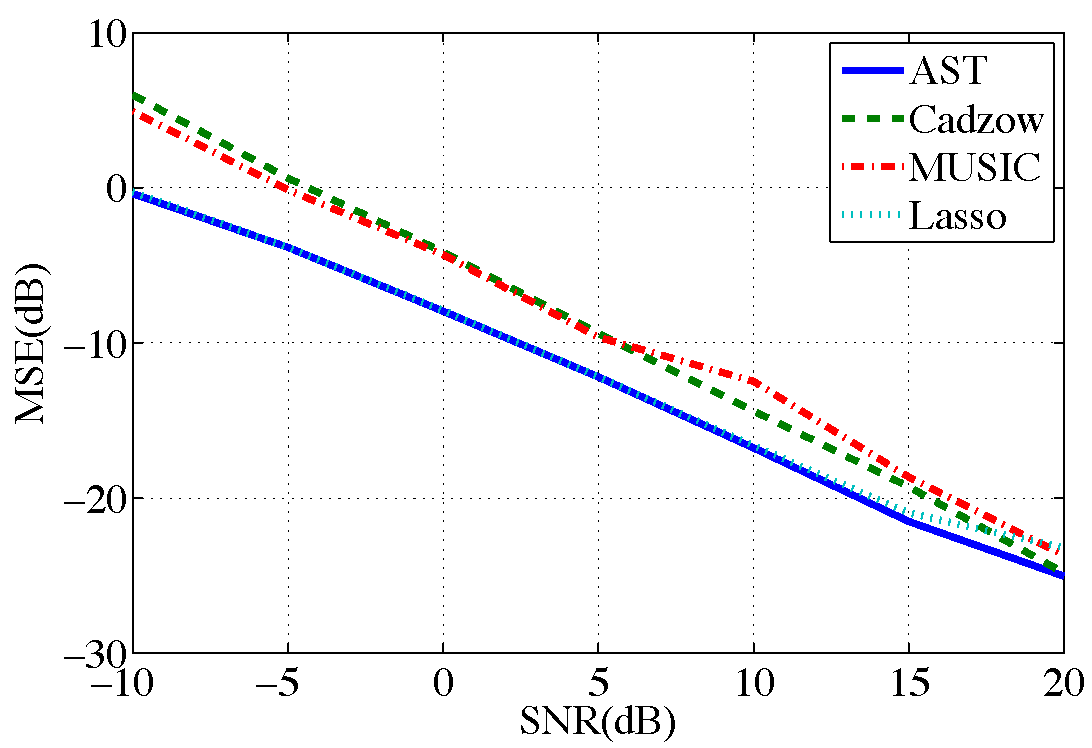
\includegraphics[width=0.5\textwidth]{figures/mse_snr_128_16_randamp} \\
	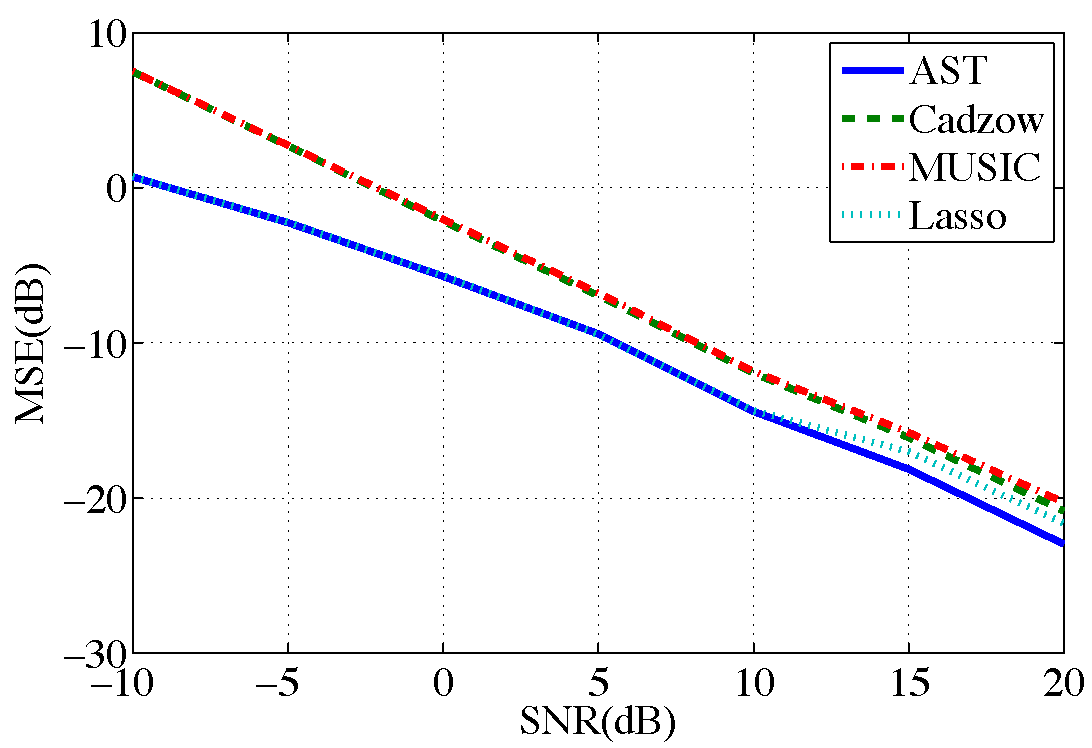
\includegraphics[width=0.5\textwidth]{figures/mse_snr_128_32_randamp}
\end{tabular}
\caption{ {\bfseries MSE vs SNR plots:} This graph compares MSE vs SNR for a subset of experiments with $n=128$ samples. From top left, clockwise, the plots are for combinations of $8$, $16$, and $32$ sinusoids with amplitudes and frequencies sampled at random.}
\label{fig:mse-snr}
\end{figure*}

In Figure~\ref{fig:mse-snr}, we show MSE vs SNR plots for a subset of
experiments when $n=128$ time samples are taken to take a closer look at the
differences. It can be seen from these plots that the performance difference
between classical algorithms such as MUSIC and Cadzow with respect to the
convex optimization based AST and Lasso is most pronounced at lower sparsity
levels. When the noise dominates the signal (SNR $\leq 0$ dB), all the
algorithms are comparable. However, AST and Lasso outperform the other
algorithms in almost every regime.


\begin{figure}[htbp]
  \begin{tabular}{cc}
	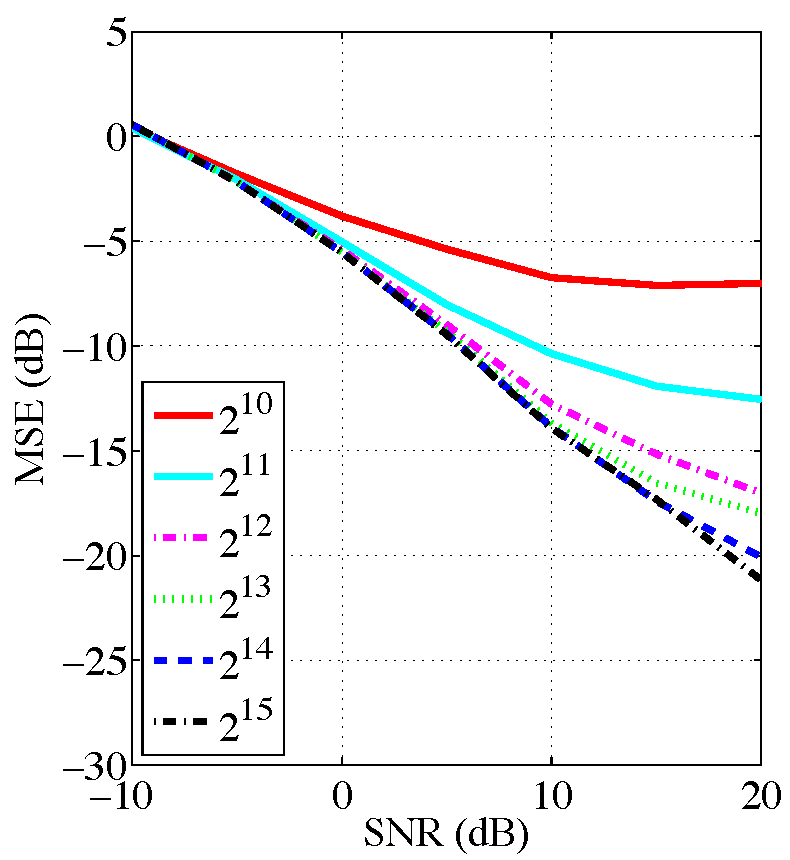
\includegraphics[trim=10mm 0mm 5mm 3mm,clip,width=0.37\linewidth]{figures/mse_snr_256_64_lasso_randamp} &
	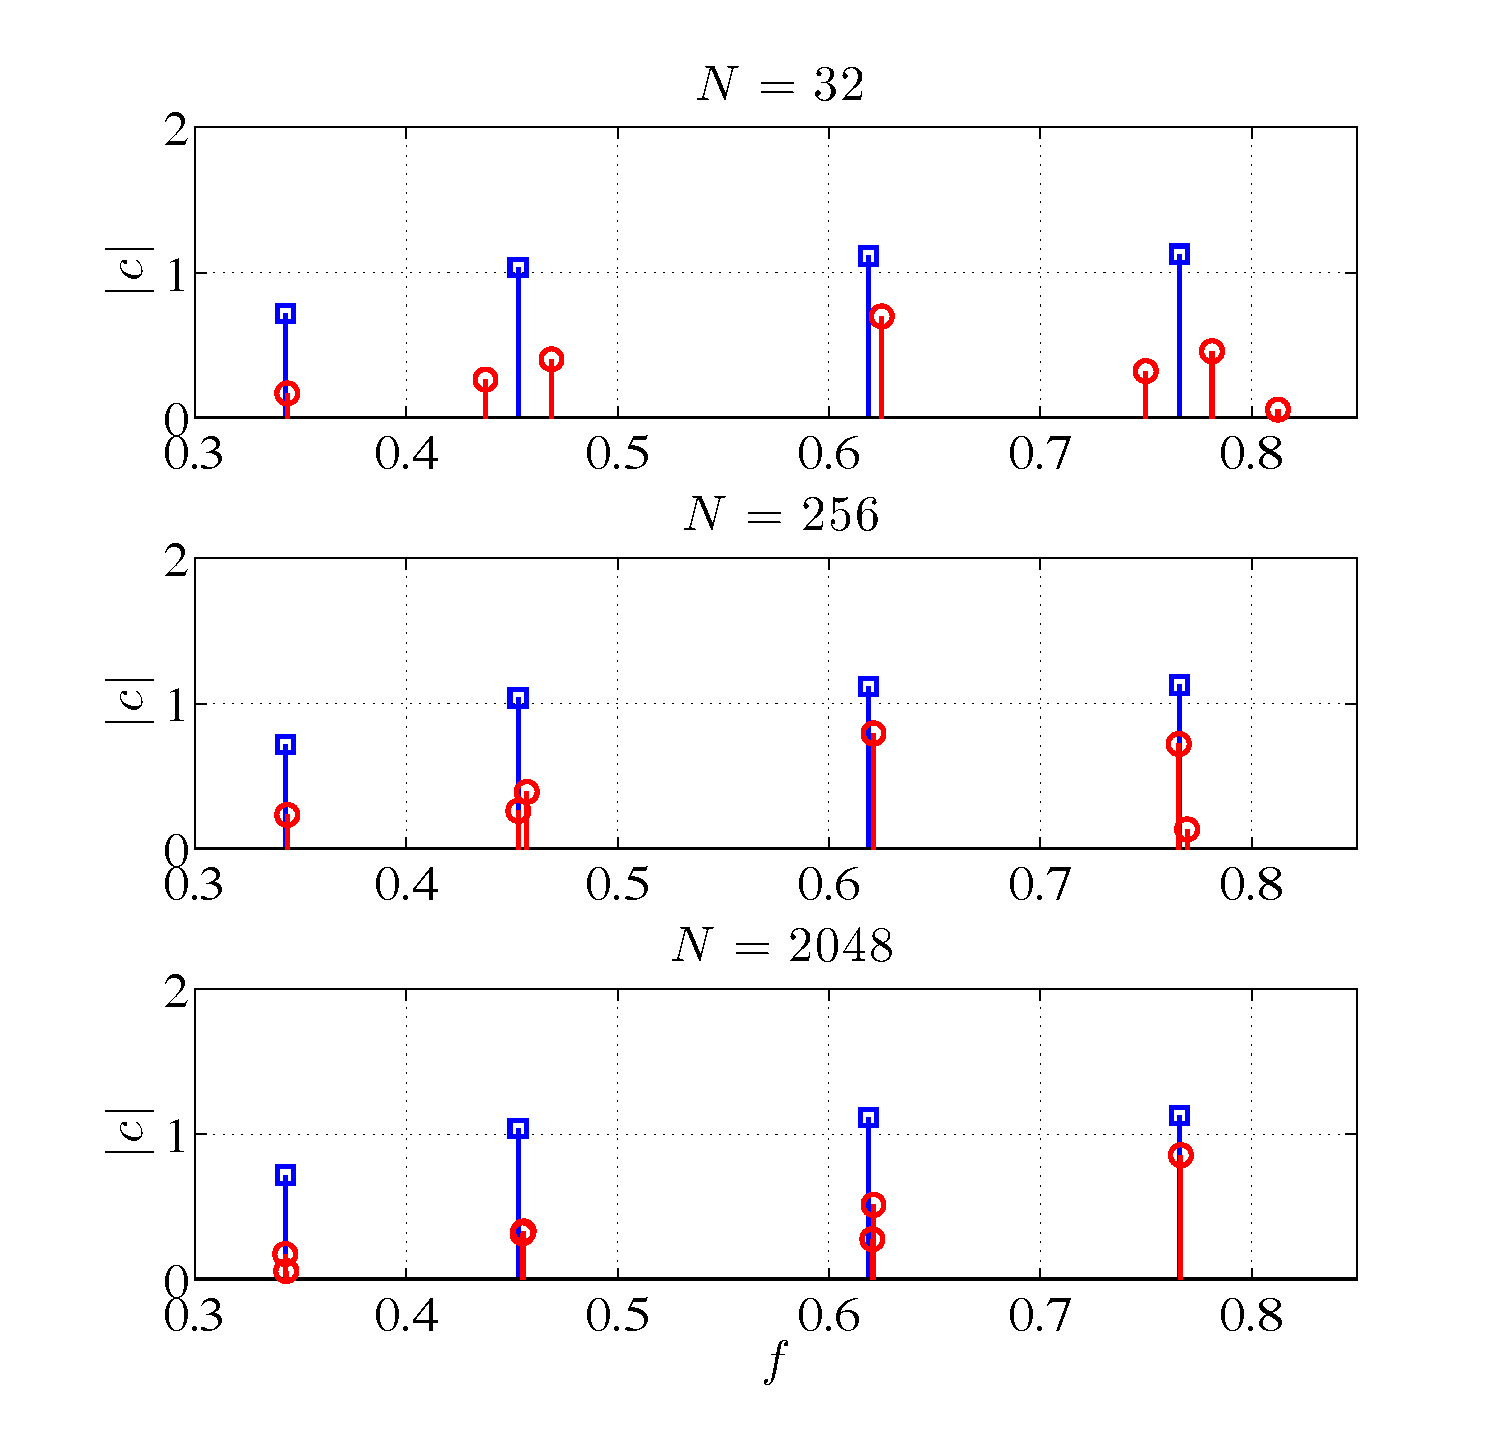
\includegraphics[trim=15mm 0mm 20mm 3mm,clip,width=0.45\linewidth]{figures/gridding} \\
(a)  & (b)
\end{tabular}
\caption{ 
(a) Plot of MSE vs SNR for Lasso at different grid sizes for a subset of experiments with $n=128, k = 16$\newline
(b) Lasso Frequency localization with $n=32, k = 4,$
SNR = $10$ dB. Blue represents the true frequencies, while red are given by Lasso. For better visualization, we threshold the Lasso solution by $10^{-6}$.}
\label{fig:lasso-compare}
\end{figure}

We note that the denoising performance of Lasso improves with increased grid
size as shown in the MSE vs SNR plot in Figure~\ref{fig:lasso-compare}(a). The
figure shows that the performance improvement for larger grid sizes is greater
at high SNRs. This is because when the noise is small, the discretization error
is more dominant and finer gridding helps to reduce this error.
Figures~\ref{fig:lasso-compare}(a) and (b) also indicate that the benefits of
increasing discretization levels are diminishing with the grid sizes, at a
higher rate in the low SNR regime, suggesting a tradeoff among grid size,
accuracy, and computational complexity.

Finally, in Figure \ref{fig:lasso-compare}(b), we provide numerical evidence
supporting the assertion that frequency localization improves with increasing
grid size. Lasso identifies more frequencies than the true ones due to basis
mismatch. However, these frequencies cluster around the true ones, and more
importantly, finer discretization improves clustering, suggesting
over-discretization coupled with clustering and peak detection as a means for
frequency localization for Lasso. This observation does not contradict the
results of \cite{cpsc} where the authors look at the full Fourier basis ($N=n$)
and the noise-free case. This is the situation where discretization effect is
most prominent. We instead look at the scenario where $N \gg n$.

In Figure~\ref{fig:msnr}, we display how the error metrics vary with
increasing SNR for AST, MUSIC and Cadzow.  We restrict these plots to the experiments with $n =
256$ samples. These plots demonstrate that AST localizes frequencies
substantially better than MUSIC and Cadzow even for low signal to noise ratios
as there is very little energy in the far region of the frequencies ($m_1$) and
has the smallest weighted mean square frequency deviation ($m_2$). Although we
have plotted the average value in these plots, we observed spikes in the plots
for Cadzow's algorithm as the average is dominated by the worst performing
instances.  These large errors are due to the numerical instability of polynomial root finding. 

\begin{figure}[htbp]
\begin{tabular}{ccc}
	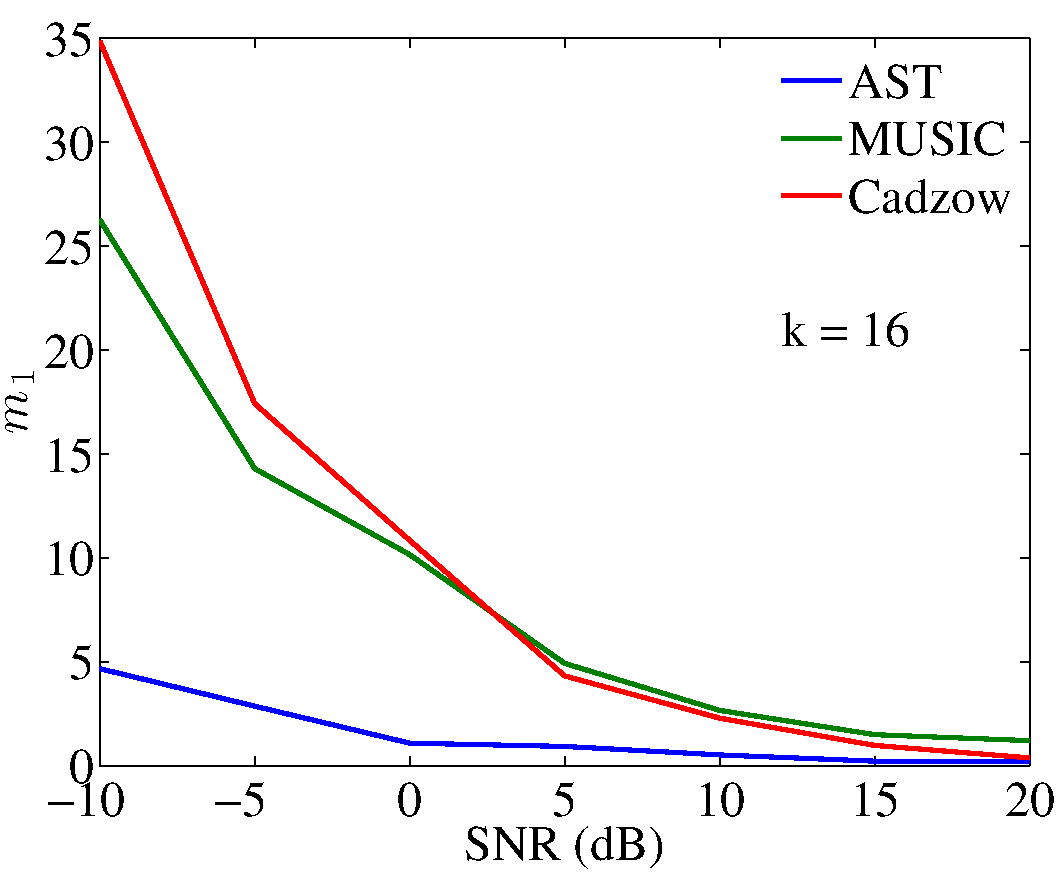
\includegraphics[height=35mm]{figures/mSNR1_16.pdf} &
	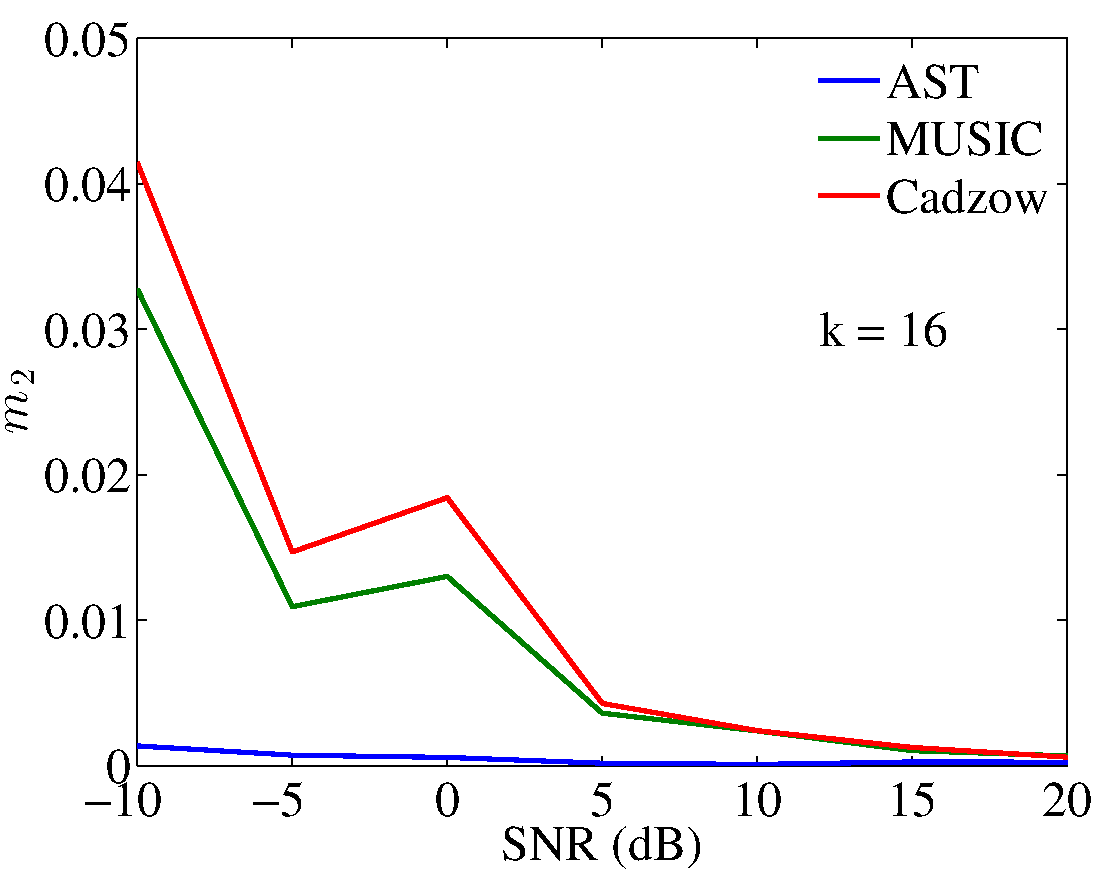
\includegraphics[height=35mm]{figures/mSNR2_16.pdf} &
	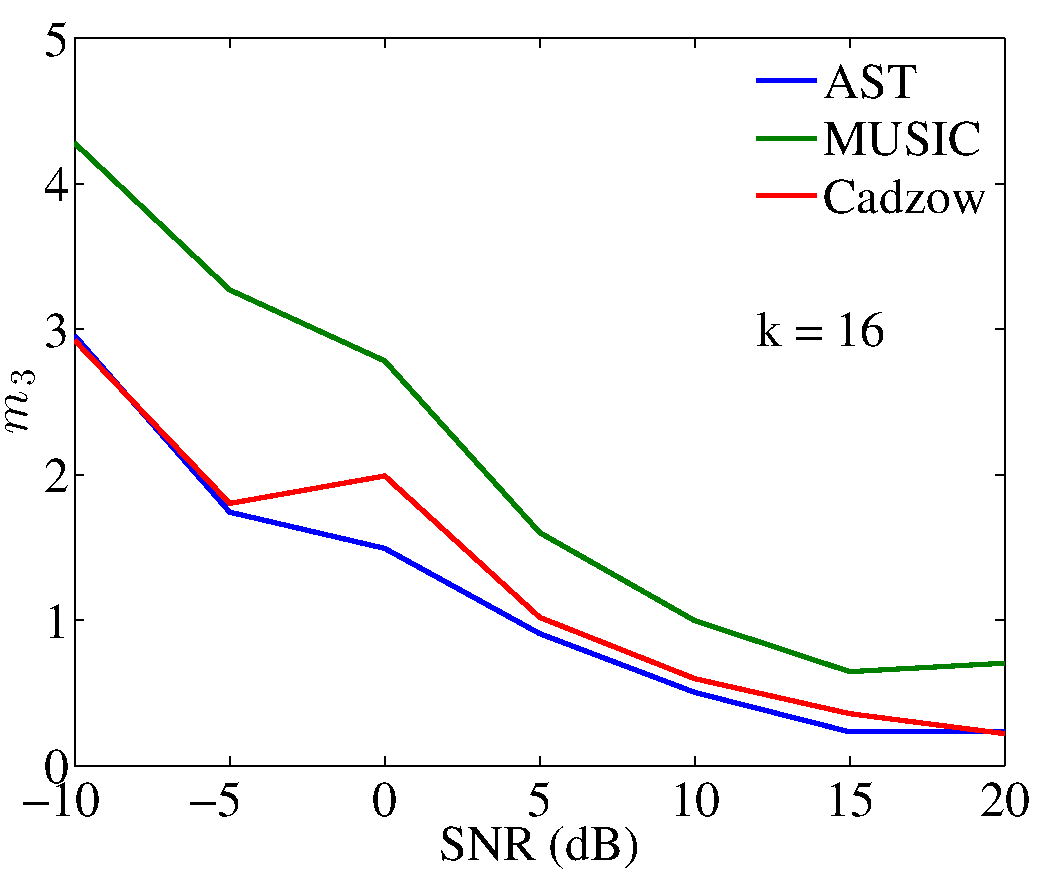
\includegraphics[height=35mm]{figures/mSNR3_16.pdf} \\
	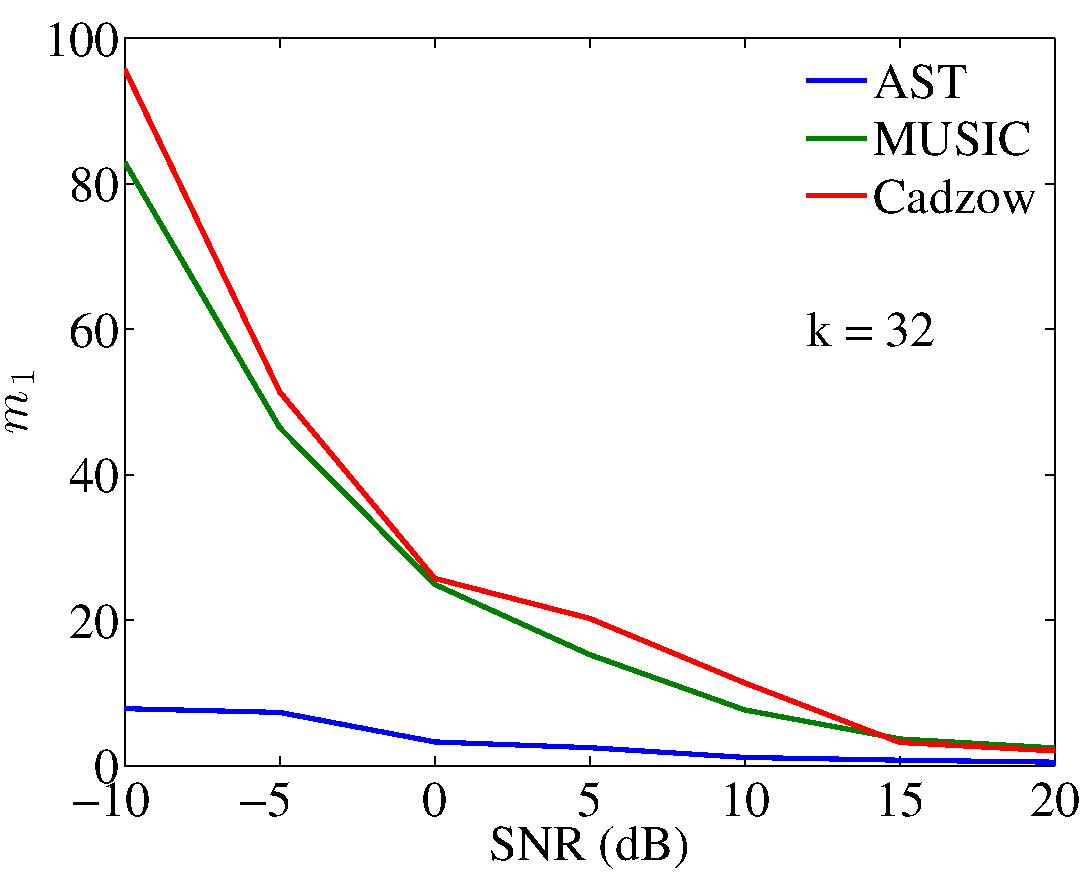
\includegraphics[height=35mm]{figures/mSNR1_32.pdf} &
	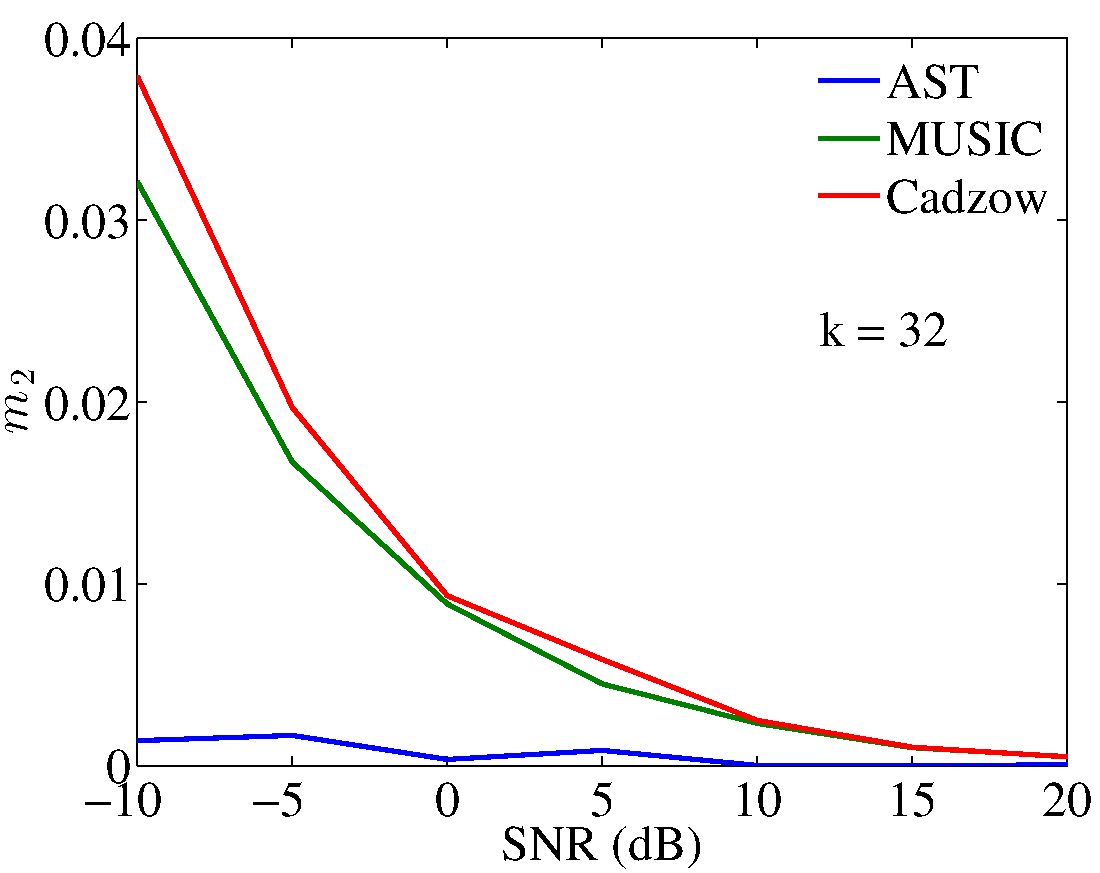
\includegraphics[height=35mm]{figures/mSNR2_32.pdf} &
	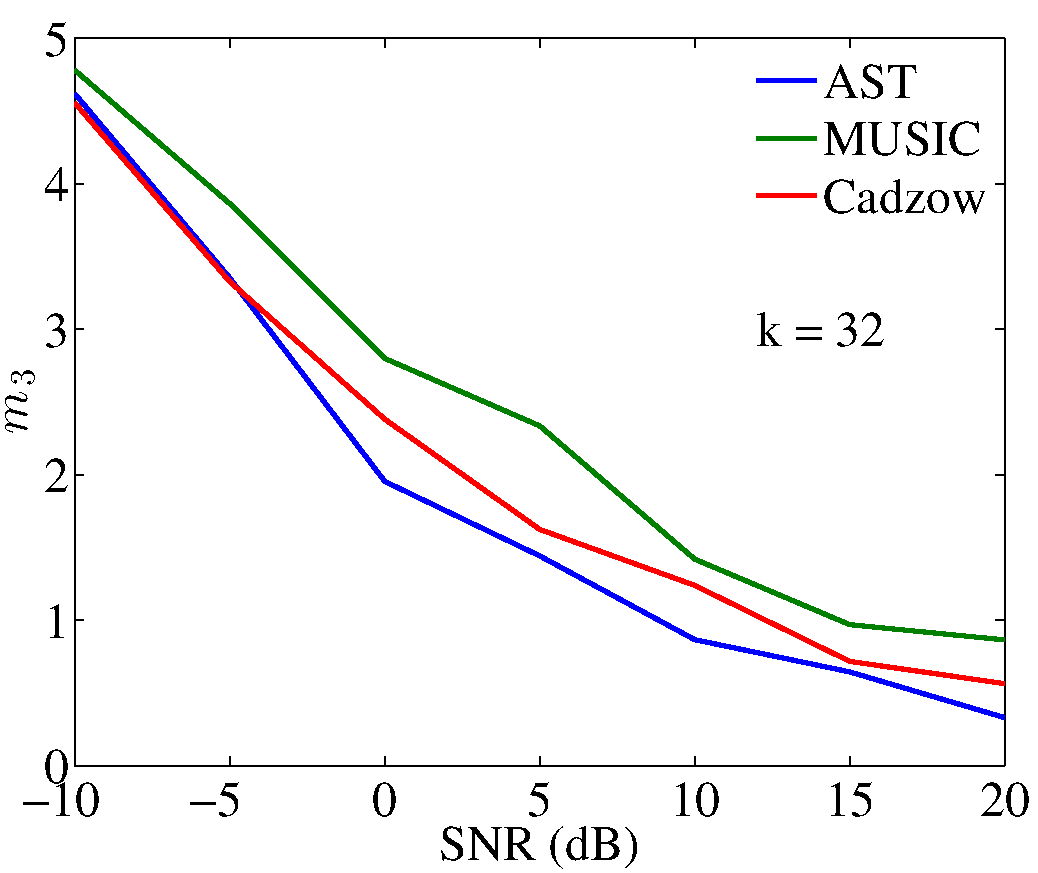
\includegraphics[height=35mm]{figures/mSNR3_32.pdf} \\
	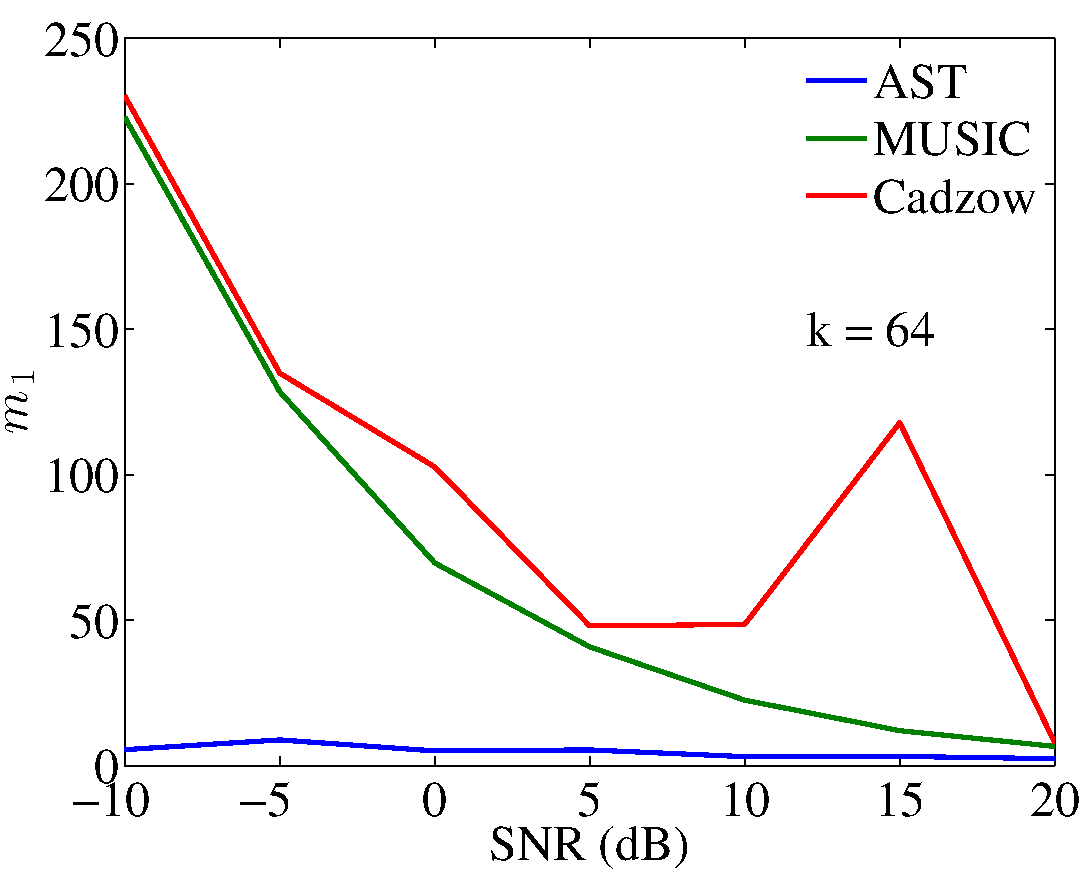
\includegraphics[height=35mm]{figures/mSNR1_64.pdf} &
	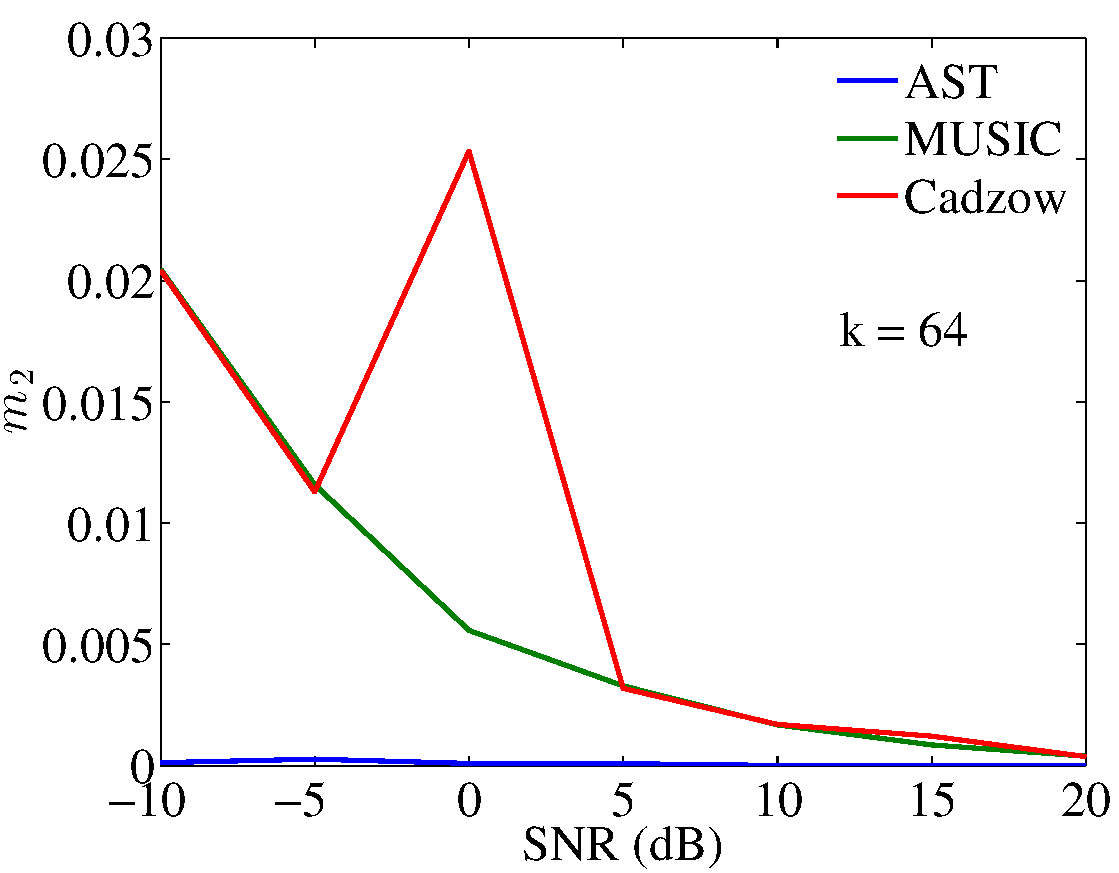
\includegraphics[height=35mm]{figures/mSNR2_64.pdf} &
	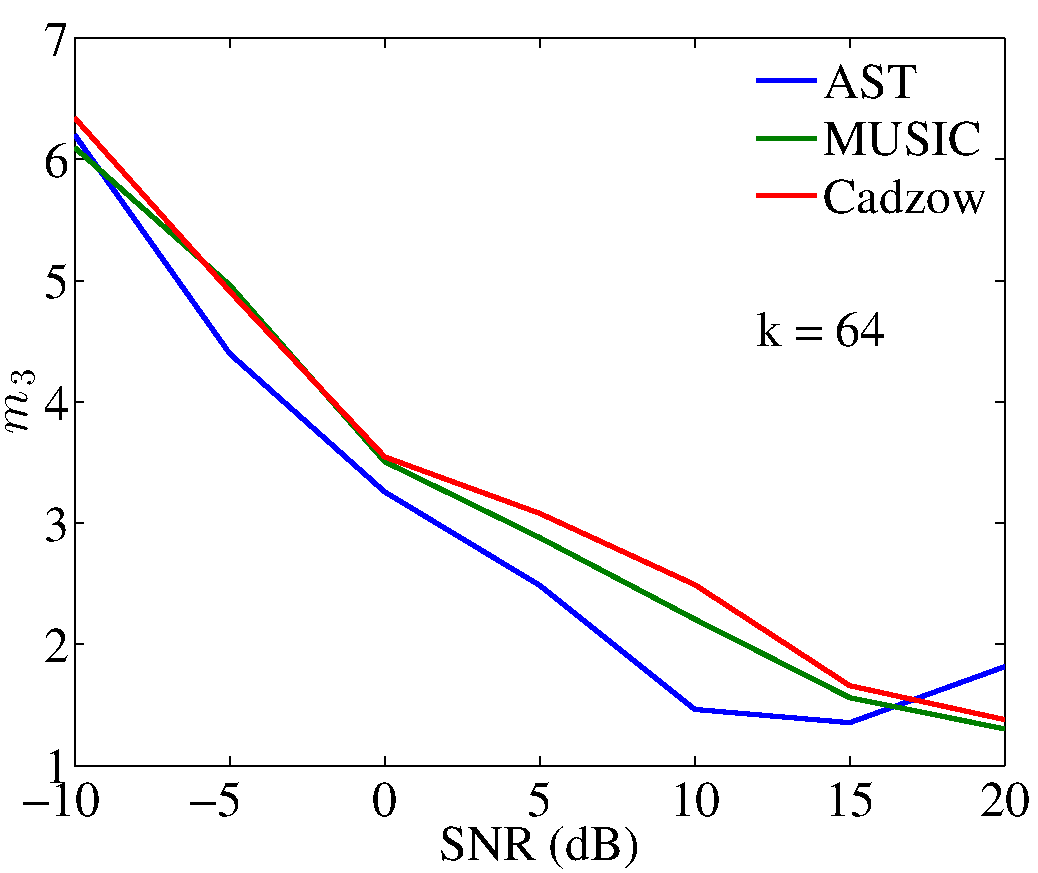
\includegraphics[height=35mm]{figures/mSNR3_64.pdf}
\end{tabular}
\caption{For $n = 256$ samples, the plots from left to right in order measure the average value over 20 random experiments for the error metrics $m_1, m_2$ and $m_3$ respectively. The top, middle and the bottom third of the plots respectively represent the subset of the experiments
with the number of frequencies $k=16, 32$ and $64$.}
\label{fig:msnr}
\end{figure}


We use \emph{performance profiles} to summarize the behavior of the various
algorithms across all of the parameter settings. Performance profiles provide a
good visual indicator of the relative performance of many algorithms under a
variety of experimental conditions\cite{dolanmore02}. Let $\mathcal{P}$ be the
set of experiments and let $\mathrm{MSE}_s(p)$ be the MSE of experiment $p \in
\mathcal{P}$ using the algorithm $s$. Then the ordinate $P_s(\beta)$ of the
graph at $\beta$ specifies the fraction of experiments where the ratio of the
MSE of the algorithm $s$ to the minimum MSE across all algorithms for the given
experiment is less than $\beta$, i.e.,

\begin{equation*}
P_s(\beta) = \frac{\mathop{\#}\left\{p \in \mathcal{P} ~:~ \mathrm{MSE}_s(p) \leq \beta \min_s \mathrm{MSE}_s(p)\right\}}{\mathop{\#}(\mathcal{P})}
\end{equation*}

\begin{figure}[htp]
\centering
\begin{tabular}{cc}
	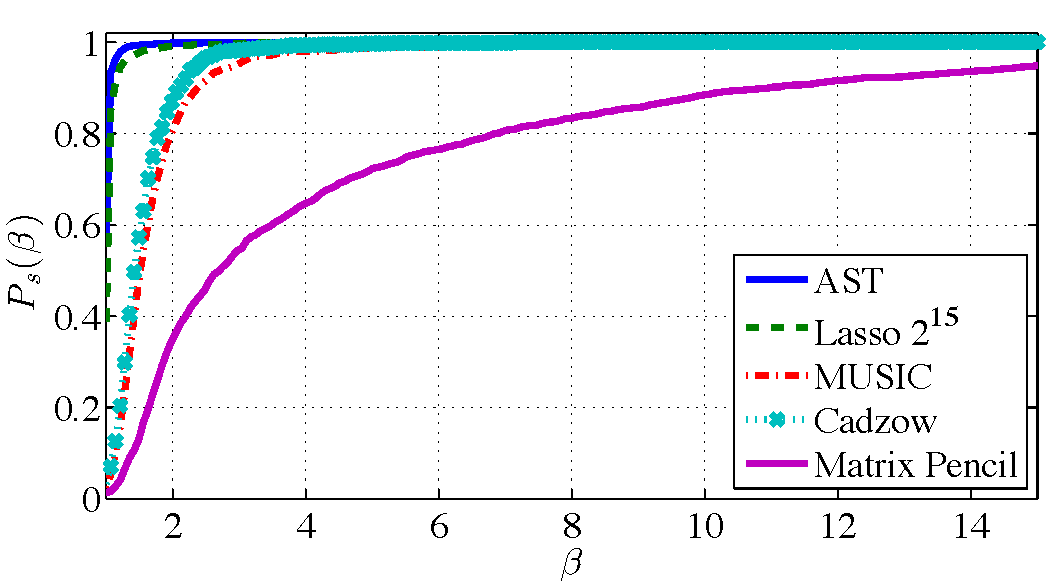
\includegraphics[height=40mm]{figures/performance_profile_randamp_color} &
	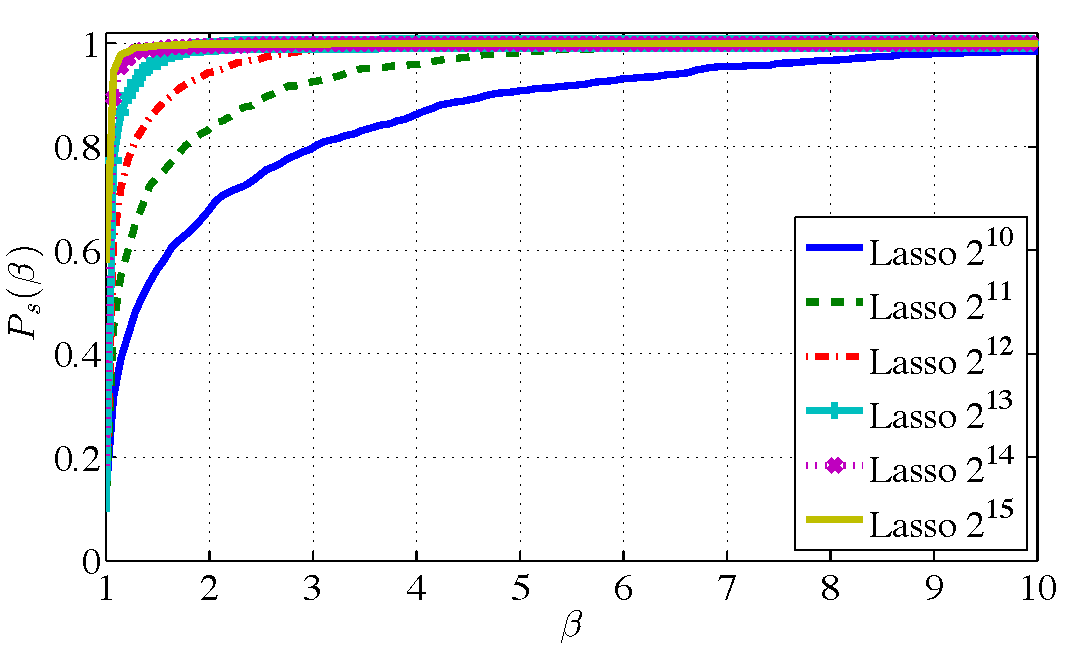
\includegraphics[trim=0mm 0mm 2mm 5mm,clip,height=40mm]{figures/performance_profile_lasso_randamp_color}\\
(a) & (b)
\end{tabular}
\caption{ (a) Performance Profile  comparing various algorithms and AST. (b) Performance profiles for Lasso with different grid sizes.}
\label{fig:pp}
\end{figure}


From the performance profile in Figure~\ref{fig:pp}(a), we see that AST is the
best performing algorithm, with Lasso coming in
second. Cadzow does not perform as well as AST, even though it is fed the true
number of sinusoids. When Cadzow is fed an incorrect $k$, even off by $1$, the
performance degrades drastically, and never provides adequate mean-squared
error. Figure~\ref{fig:pp}(b) shows that the denoising performance
improves  with grid size.

\begin{figure}[htp]
\begin{tabular}{ccc}
	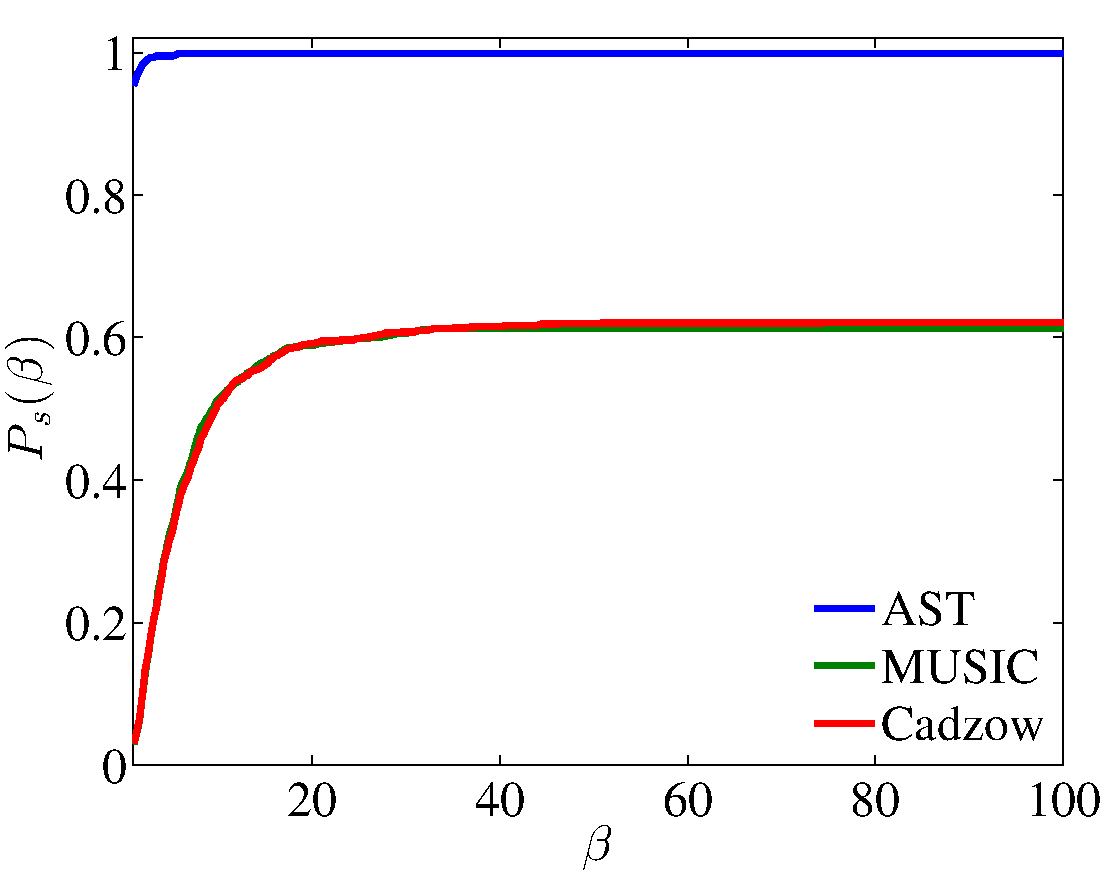
\includegraphics[height=35mm]{figures/m1_pp.pdf} &
	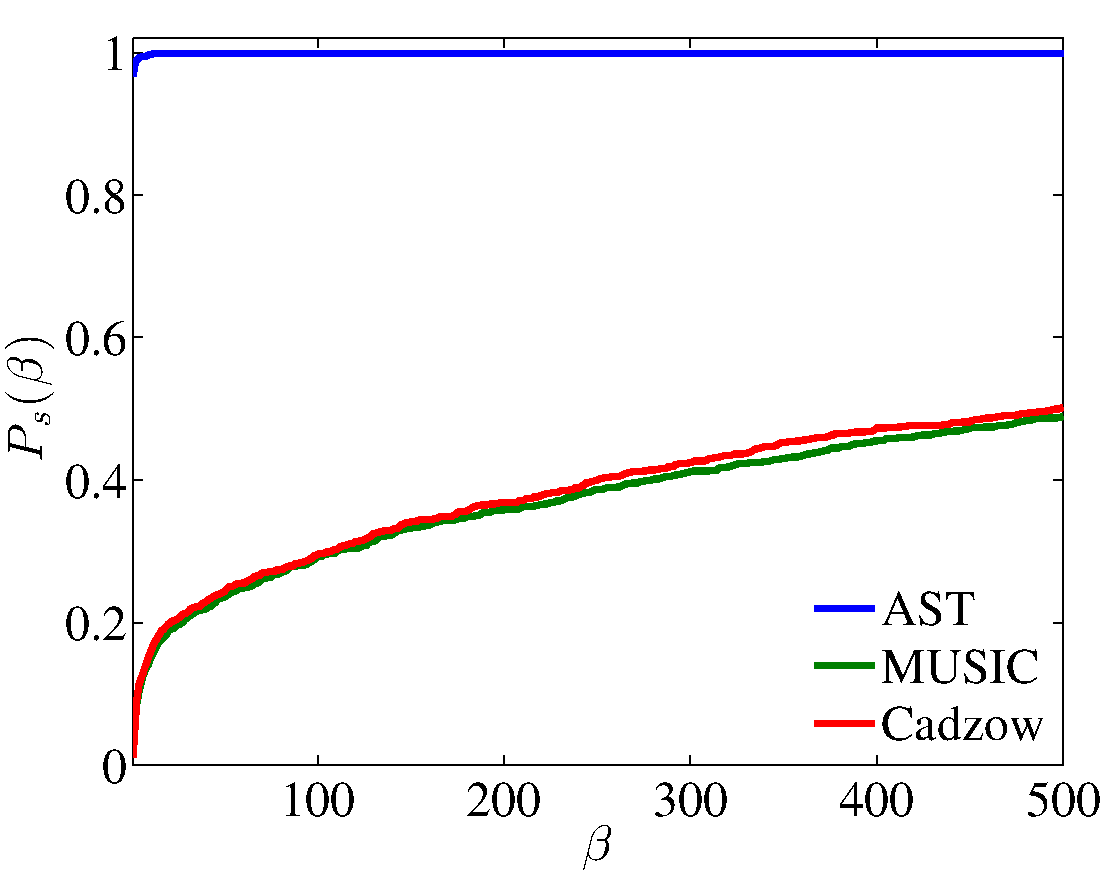
\includegraphics[height=35mm]{figures/m2_pp.pdf} &
	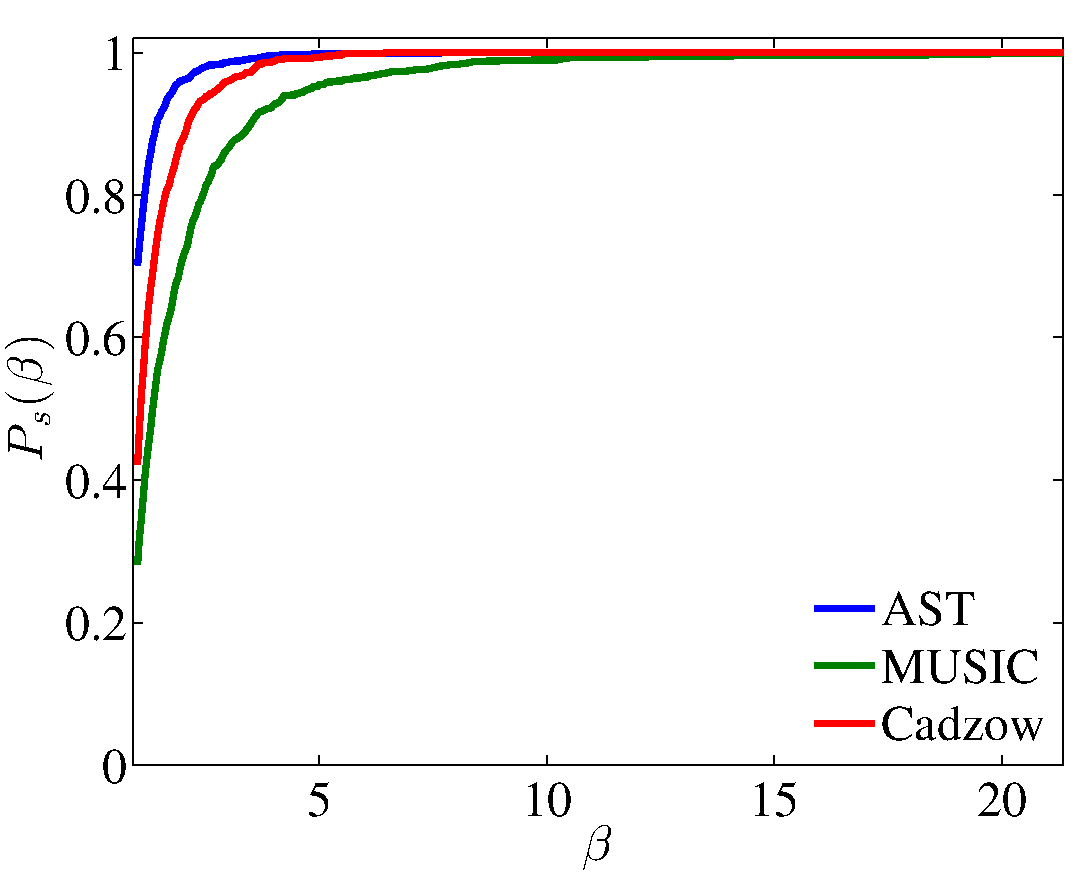
\includegraphics[height=35mm]{figures/m3_pp.pdf}\\
	(a) $m_1$ & (b) $m_2$ & (c) $m_3$
\end{tabular}
\caption{ Performance Profiles for AST, MUSIC and Cadzow.
(a) Sum of the absolute value of amplitudes in the far region ($m_1$)
(b) The weighted frequency localization error, $m_2$
(c) Error in approximation of amplitudes in the near region, $m_3$ }
\label{fig:pp}
\end{figure}

The performance profiles in Figure~\ref{fig:pp} show that AST is the best
performing algorithm for all the three metrics.  AST in fact outperforms
MUSIC and Cadzow by a substantial margin for metrics $m_1$ and $m_2$. 


\section{Conclusion and Future Work}\label{sec:conclusions}

\todo{Modify Conclusions by merging in with Minimax and Removing Stuff}

The Atomic norm formulation of line spectral estimation provides several
advantages over prior approaches. By performing the
analysis in the continuous domain we were able to derive simple closed form
rates using fairly straightforward techniques.We only grid the unit circle at the very end of
our analysis and determine the loss incurred from discretization. This approach
allowed us to circumvent some of the more complicated theoretical arguments
that arise when using concepts from compressed sensing or random matrix theory.

This work provides several interesting possible future directions, both in line
spectral estimation and in signal processing in general. We conclude with a
short outline of some of the possibilities.

\paragraph{Fast Rates} Determining checkable conditions on the cones in
Section~\ref{sec:convergence-rate} for the atomic norm problem is a major open
problem. Our experiments suggest that when the frequencies are spread out, AST
performs much better with a slightly larger regularization parameter.  This observation was also made in the model-based compressed sensing literature~\cite{duartescs}.  Moreover, Cand\`es and Fernandez Granda also needed a spread assumption to prove their theories.

This evidence together suggests the \emph{fast rate} developed in Section~\ref{sec:convergence-rate} may be active for signals with well separated frequenies. Determining concrete conditions on the signal $x^\star$ that ensure this fast rate require techniques for estimating the parameter $\phi$ in~\eq{compatibility}. Such an
investigation should be accompanied by a determination of the minimax rates for
line spectral estimation. Such minimax rates would shed further light on the
rates achievable for line spectral estimation.

\paragraph{Moments Supported Inside the Disk} Our work also naturally extends
to moment problems where the atomic measures are supported on the unit disk in
the complex plane. These problems arise naturally in controls and systems
theory and include model order reduction, system identification, and control
design. Applying the standard program developed in
Section~\ref{sec:abstract-denoising} provides a new look at these classic
operator theory problems in control theory. It would be of significant
importance to develop specialized atomic-norm denoising algorithms for control
theoretic problems. Such an approach could yield novel statistical bounds for
estimation of rational functions and $\mathcal{H}_\infty$-norm approximations.

\paragraph{Other Denoising Models} Our abstract denoising results in
Section~\ref{sec:abstract-denoising} apply to any atomic models and it is worth
investigating their applicability for other models in statistical signal
processing. For instance, it might be possible to pose a scheme for denoising a
signal corrupted by multipath reflections. Here, the atoms might be all time
and frequency shifted versions of some known signal. It remains to be seen what
new insights in statistical signal processing can be gleaned from our unified
approach to denoising.


\chapter{System Identification} 

Identifying dynamical systems from noisy observation of their input-output
behavior is of fundamental importance in systems and control theory. Often
times models derived from physical first principles are not available to the
control engineering, and computing a surrogate model from data is essential to
the design of a control system. System identification from data is thus
ubiquitous in problem domains ranging from process engineering, dynamic
modeling of mechanical and aerospace systems, and systems biology. Though there
are a myriad of approaches and excellent texts on the subject (see, for
example~\cite{LjungBook}), there is still no universally agreed upon approach
for this problem. One reason is that quantifying the interplay between system
parameters, measurement noise, and model mismatch tends to be challenging.

We draw novel connections between contemporary high-dimensional statistics,
operator theory, and linear systems theory to prove consistent estimators of
linear systems from small measurement sets. In particular, building on recent
studies of \emph{atomic norms} in estimation
theory~\cite{CRPW10,BhaskarAllerton11}, we propose a penalty function which
encourages estimated models to have small McMillan degree.

A related family of system identification techniques use finite sample Hankel
matrices to estimate dynamical system models, using either singular value
decompositions (e.g,~\cite{Verhaegen92,Overschee94}) or semidefinite
programming~\cite{Fazel01,Liu08,Smith12,Fazel11}. In all of these techniques,
no statistical guarantees were given about the quality of estimation with
finite noisy data, and it was difficult to determine how sensitive these
methods were to the hidden system parameters or measurement noise. Moreover,
since these problems were dealing with finite, truncated Hankel matrices, it is
never certain if the size of the Hankel matrix is sufficient to reveal the true
McMillan degree. Moreover, the techniques based on semidefinite programming are
challenging to scale to very large problems, as their complexity grows
superlinearly with the number of measurements.

In contrast, the atomic norm regularizer proposed in this chapter is not only
equivalent to the sum of the Hankel singular values (the Hankel nuclear norm),
but is also well approximated by a finite dimensional, $\ell_1$ minimization
problem. We show that solving least-squares problems regularized by our atomic
norm is consistent, and scales gracefully with the stability radius, the
McMillan degree of the system to be identified, and the number of measurements.
Our numerical experiments validate these theoretical underpinnings, and show
that our method has great promise to provide concrete estimates on the hard
limits of estimating linear systems.

\subsection{Notation}\label{sec:notation}

We adopt standard notation; $\D$ and $\bbS$ will denote respectively the open
unit ball and the unit circle in the complex plane $\C$ . $\cH_2$ and
$\cH_\infty$ will denote the Hardy spaces of functions analytic outside $\D$,
with the norms

\[\|f\|_{\cH_2} = \tfrac{1}{2\pi} \int_0^{2\pi} |f(e^{i\theta})|^2 d\theta~~~~~\mbox{and}~~~~~\|f\|_{\cH_\infty} = \sup_{z\in\bbS} |f(z)|\]
respectively.  $\ell_2([a,b])$ will denote the set of square summable sequences on the integers in $[a, b]$.

\section{Atomic Decompositions of Transfer Functions}\label{sec:atomic-def}
We restrict our attention to SISO systems in this manuscript, as this will simplify the presentation.  However, we will describe in the discussion how to extend our techniques to MIMO systems.  Suppose we wish to estimate a SISO, LTI system with transfer function $G_\star(z)$ from a finite collection of measurements $y=\Phi(G_\star)$.  The set of all transfer functions is an infinite dimensional space, so reconstructing $G_\star$ from this data is ill-posed.  In order to make it well posed, a common regularization approach constructs a penalty function $\operatorname{pen}(\cdot)$ that encourages ``low-complexity'' models and solves the optimization problem
\begin{equation}\label{eq:regularized}
	\minimize_G~\|\Phi(G)-y\|_2^2 + \mu \operatorname{pen}(G) \,.
\end{equation}
This formulation uses the parameter $\mu$ to balance between model complexity and fidelity to the data.  The least-squares cost can be modified to other convex loss functions if knowledge about measurement noise is available (as in~\cite{Smith12,Paganini96}), though in general it is less clear how to design a good penalty function.

In many applications, we know that the true model can be decomposed as a linear combination of very simple building blocks.  For instance, sparse vectors can be written as short linear combinations of vectors from some discrete dictionary and low-rank matrices can be written as a sum of a few rank-one factors.  In~\cite{CRPW10}, Chandraskearan et al. proposed a universal heuristic for constructing regularizers based on such prior information.  If we assumed that 
\[
	G_\star = \sum_{i=1}^r c_i a_i\,,~\mbox{for some}~a_i\in\cA,c_i\in \C\,,
\]
where $\cA$ is an origin-symmetric set of ``atoms'' normalized to have unit norm and $r$ is relatively small, then the appropriate penalty function is the guage function (or the Minkowski functional) induced by the atomic set $\cA$:
\begin{equation}\label{eq:atomic-norm-def}
\begin{split}
	\|G\|_{\cA}: & = \inf\left\{ t \; : \; G \in t\text{ conv}(\cA)  \right\}  =\inf\left\{ \sum_{a\in \cA} |c_a|~:~G = \sum_{a\in \cA} c_a a\right\}\,.
\end{split}
\end{equation}
In~\cite{CRPW10}, it is shown that minimizing the atomic norm subject to compressed measurements yielded the tightest known bounds for recovering many classes of models from linear measurements. Moreover, in~\cite{BhaskarAllerton11}, the atomic norm regularizer was studied in the context of denoising problems and was found to produce consistent estimates at nearly optimal estimation error rates for many classes of atoms.

To apply these atomic norm techniques to system identification, we must first determine the appropriate set of atoms.  For discrete time LTI systems with small McMillan degree, we can always decompose any finite dimensional, strictly proper system $G(z)$ as:
$$
G(z)=\sum_{i=1}^{s} \frac{c_i}{z-a_i}\,.
$$
via a partial fraction expansion.  Hence, it makes sense that our set of atoms should be single-pole transfer functions.  We propose the following atomic set for linear systems
\[
\cA = \left\{ \varphi_{w}(z) = \frac{1-|w|^2}{z-w} ~:~w\in \D\right\}\,.
\]
The numerator is normalized so that the Hankel norm of each atom is $1$.  See the discussion in Section~\ref{sec:hankel} for precisely why this normalization is desirable.

The atomic norm penalty function associated with these atoms is 
\begin{equation}\label{eq:atomic-def}
	\| G(z) \|_{\cA} = \inf \left\{ \sum_{w\in \D} |c_w| ~:~ G(z) = \sum_{w\in\D} \frac{c_w (1-|w|^2)}{z-w}\right\}\,,
\end{equation}
where the summation implies that only a countable number of terms have nonzero coefficients $c_w$.  This expression finds the decomposition of $G(z)$ into a linear combination of single pole systems such that the $\ell_1$ norm, weighted by the norms of the single poles, is as small as possible.

With this penalty function in hand, we now turn to analyzing its utility.  In Section~\ref{sec:hankel}, we first show that for most systems of interest $\|G\|_{\cA}$ is a well-defined, bounded quantity.  Moreover, we will show that the atomic norm is equivalent to the nuclear norm of the Hankel operator associated with  $G$.  Hence, the models that are preferred by our penalty function will have low-rank Hankel operators, and thus low McMillan degrees.

In Section~\ref{sec:computation}, we turn to computation, demonstrating practical algorithms for approximating atomic norm regularization problems for several classes of measurements.  We will show that with finite data, our atomic norm minimization problem is well-approximated by a finite-dimensional $\ell_1$ norm regularization problem.  In particular, using specialized algorithms adapted to the solution of the LASSO~\cite{Wright09}, we can solve atomic norm regularization problems in time competitive with respect to techniques that regularize with the nuclear norm and SVD-based subspace identification methods.

Finally, we analyze the statistical performance of atomic norm minimization in Section~\ref{sec:statistics}.  We show that our algorithm is asymptotically consistent over several measurement ensembles of interest.  We focus on sampling the transfer function on the unit circle and present $\cH_2$ error bounds in terms of the stability radius, Hankel singular values, $\cH_{\infty}$ norm, and McMillan degree of the system to be estimated.

\section{The Hankel Nuclear Norm and Atomic Norm Minimization}\label{sec:hankel}

Let us first show that most LTI systems of interest do indeed have finite atomic norm, and, moreover, that the atomic norm is closely connected with the sum of the Hankel singular values.

\subsection{Preliminaries: the Hankel operator}\label{sec:hankel-defs}
Recall that the \emph{Hankel operator}, $\Gamma_G$, of the transfer function $G$ is defined as the mapping from the past to the future under the transfer function $G$.  Given a signal $u$ supported on $(-\infty,-1]$, the output under $G$ is given by $g * u$ where ``$*$'' denotes convolution and $g$ is the impulse response of $G$: 
\[
	G(z) = \sum_{k=1}^\infty g_k z^{-k}\,.
\]
$\Gamma_G$ is then simply the projection of $g*u$ onto $[0,\infty)$.  An introduction to Hankel operators in control theory can be found in~\cite[Chapter 4]{DullerudPaganiniBook} or~\cite[Chapter 7]{Zhou95}.

The \emph{Hankel norm} of $G$ is the operator norm of $\Gamma_G$ considered as an operator mapping $\ell_2(-\infty,-1]$ to $\ell_2[0,\infty)$. The \emph{Hankel nuclear norm} of $G$ is the nuclear norm (aka the trace norm or Schatten $1$-norm) of $\Gamma_G$.  To be precise, an operator $T$ is in the \emph{trace class} $S_1$ if the trace of $(T^*T)^{1/2}$ is finite.  This implies first that $T$ is a compact operator and admits a singular value decomposition
\begin{equation*}
    T(f) = \sum_{i=1}^\infty \sigma_i \langle v_i, f \rangle u_i \,.
\end{equation*}
The sequence $\sigma_i$ are called the \emph{Hankel singular values} of $T$.  Moreover, the Schatten $1$-norm of $T$ is given by
\begin{equation*}
    \|T\|_1 = \trace\left((T^*T)^{1/2}\right) =
    \sum_{i=1}^\infty \sigma_i\,.
\end{equation*}

\subsection{The atomic norm is equivalent to the Hankel nuclear norm}
The rank of the Hankel operator determines the McMillan degree
of the linear system defined by $G$.  Rank minimization is notoriously computationally challenging (see~\cite{Recht10} for a discussion), and we don't expect to be able to directly penalize the norm of the Hankel operator in implementations.  Thus, as is common, a reasonable heuristic for minimizing the rank of the Hankel operator would be to minimize the sum of the Hankel singular values, i.e., to minimize the Schatten $1$-norm of the Hankel operator.  For rational transfer functions, we can compute the Hankel nuclear norm via a balanced realization~\cite{Zhou95}.  On the other hand, while the maximal Hankel singular value can be written variationally as an LMI, we are not aware of any such semidefinite programming formulations for the Hankel nuclear norm.  

The following theorem provides a path towards minimizing the Hankel nuclear norm, minimizing the atomic norm $\|G(z)\|_{\cA}$ as a proxy.  Indeed, from the view of Banach space theory, the atomic norm is~\emph{equivalent} to the Hankel nuclear norm.

\begin{theorem}\label{thm:hankel-nuclearity}
Let $G \in \cH_2$.  Then $\Gamma_G$ is trace class if and only if there exists a sequence $\{\lambda_k\} \in \ell_1$ and a
    sequence $\{w_k\}$ with $w_k \in \D$ such that
\begin{equation}\label{eq:kernel-form}
    g(z) = \sum_{i=1}^\infty \lambda_k \frac{1-|w_k|^2}{z-w_k}\,.
    \end{equation}
Moreover, we have the following chain of inequalities
\begin{equation}\label{eq:norm-ineq-chain}
\tfrac{\pi}{8}\|G\|_{\cA} \leq  \|\Gamma_G\|_1 \leq
\|G\|_{\cA} 
\end{equation}
where  $\|G\|_{\cA}$ is given by~\eq{atomic-norm-def}.
\end{theorem}
\emph{Proof Outline}  Theorem~\ref{thm:hankel-nuclearity} follows by carefully combining several different results from operator theory. Peller first showed that transfer functions with trace class Hankel operators formed a \emph{Besov space}~\cite{Peller79}. Peller's argument can be found in his book~\cite{PellerHankelBook}. The atomic decomposition of such operators is due to Coifman and Rochberg~\cite{Coifman80}. The norm bounds~\eq{norm-ineq-chain} were proven by Bonsall and Walsh~\cite{Bonsall86}. There they show that the $\tfrac{\pi}{8}$ is the best possible lower bound.  They also show that if $\|\Gamma_g\|_1\leq C\|g\|_{\cA}$ for all $g$, then $C$ must be at least $\tfrac{1}{2}$, so the chain of inequalities is nearly optimal. A concise presentation of the full argument can be found  in~\cite{PartingtonHankelBook}. A modern perspective using the theory of reproducing kernels can be found in~\cite{ZhuBook}. 
\vspace{1mm}

\noindent Theorem~\ref{thm:hankel-nuclearity} asserts that a transfer function has a finite atomic norm if and only if the sum of its Hankel singular values is finite.  In particular, this means that every rational transfer function has a finite atomic norm.  More importantly, the atomic norm is equivalent to the Hankel nuclear norm.  Thus if we can approximately solve atomic norm-minimization, we can approximately solve Hankel nuclear norm minimization and vice-versa.

\section{Statistical Bounds}\label{sec:statistics}
Let $\cL_i: \cH \mapsto \C $ be a linear functional that serves as a measurement operator for the system $H(z)$.  In this section, let us suppose that we obtain noisy measurements of the form
$$
y_i=\cL_i \left( H(z) \right) +\omega_i \qquad i=1, \ldots, n.
$$
where $\omega_i$ is a noise sequence consisting of independent, identically distributed random variables.  In this section, we will specialize our results to the case where $\cL$ returns samples from the frequency response at uniformly spaced frequencies:
$$
\cL_k(H(z))=H(z_k), \qquad z_k=e^{\frac{2 \pi i k}{m} }, \; k=1, \ldots, n.
$$
While the techniques here extend to other measurement ensembles, they will be explored in a longer version of the paper.
%
%
%We only prove one theorem to illustrate the techniques required to analyze a general set of measurements.  The theorem will change with different grindings of the disk, measurements, and noise models.  We will study other examples in future work.

Our goal in this section is to prove that solving the DAST optimization problem yields a good approximation to the transfer function we are probing. The following theorem provides a precise statistical guarantee on the performance of our algorithm.
\begin{theorem}\label{thm:estimation}  Let $G_\star$ be a strictly proper transfer function with bounded Hankel nuclear norm. Suppose the noise sequence $\omega_i$ is i.i.d. Gaussian with mean zero and variance $\sigma^2$.  Choose $\delta \in (0,1)$ and set $\epsilon = \frac{\pi (1-\rho)\delta}{16 \rho}$.  Let $\D_\rho^{(\epsilon)}$ be as in Proposition~\ref{prop:grid} and let $\hat{c}$ be the optimal solution of~\eq{DAST} with 
\[
\mu=2\sigma \sqrt{ n \log \left(\frac{11 \rho^2}{\delta(1-\rho)} \right)}\,.
\]
Set $\hat{G}(z) = \sum_{w \in \D_{\rho}^{(\epsilon)}} \hat{c}_w \frac{1-|w|^2}{z-w}$.  Then if the set of vectors $\{\cL(\varphi_a)\in \R^n~:~a\in\D_{\rho}^{(\epsilon)}\}$ spans $\R^n$, we have 
\[
\begin{aligned}
	&\|\hat{G}(z)-G_{\star}(z)\|_{\cH_2}^2 \leq  
	186 \frac{1+\rho}{1-\rho} \left( \sqrt{\sigma^2 \log\left(\frac{11 \rho^2}{(1-\rho)\epsilon}\right)}\sqrt{\frac{\|\Gamma_{G_\star}\|_{1}^2}{n(1-\delta)^2} } + \frac{4\|\Gamma_{G_\star}\|_{1}^2}{\pi n(1-\delta)^2}   \right)
	\end{aligned}
\]
with probability $1-e^{-o(n)}$.
\end{theorem}
\begin{corollary} \label{cor:1}
There is a quantity $C$ depending on $\rho$ and $\sigma$ such that for sufficiently large $n$
$$\|\hat{G}(z)-G_{\star}(z)\|_{\cH_2}^2\ \leq C \| \Gamma_{G_{\star}} \|_1 n^{-\frac{1}{2}}$$
with probability exceeding $1-e^{-o(n)}$.
\end{corollary}
\noindent Before we describe how to prove this theorem and its corollary, let us first unpack the features.  First of all, the right hand side is a parameter of the number of samples, the Hankel nuclear norm of the true system, and the stability radius of the true system.  Also, if the McMillan degree of $G_\star(z)$ is $d$, then we can upper bound the Hankel nuclear norm by the product of the McMillan degree and the Hankel norm of $G_\star$: $\|\Gamma_{G_\star}\|_1 \leq d \|\Gamma_{G_\star}\|$.
Second, note that as $n$ tends to infinity, the right hand side tends to zero.  In particular, this means that our discretized algorithm is consistent, and we can quantify the worst case convergence rate.  

The proof of theorem~\ref{thm:estimation} is provided in the appendix.  We prove this theorem by first upper bounding the $\cH_2$ in terms of the mean square error on the observed samples.  We show that this empirical mean square error can be upper bounded in terms of the Hankel nuclear norm of $G_\star$ times the \emph{dual atomic norm} of the noise sequence $\omega$.  We estimate this norm, and in the process compute the optimal value of the regularization parameter.  Putting these pieces together yields our main result.

\section{Conclusion}\label{sec:conclusion}

By using the atomic norm framework of~\cite{CRPW10}, we were able to posit a reasonable regularizer for linear systems, understand the computational demands of such a regularizer, and analyze its statistical performance.  Since it is closely connected to the Hankel nuclear norm but is computationally more practical, we believe that our atomic norm will be useful in a variety of practical implementations and also in theoretical analysis.  However, there are still several outstanding questions to address before we fully understand the potential of this norm.  We list several of these open problems here.

\paragraph{Other measurement ensembles} Our analysis in Section~\ref{sec:statistics} focused on the particular case of sampling the frequency response at regular intervals.  By focusing on this example, we were able illustrate the critical ingredients to computing convergence rates.  First, we needed to show that our measurement error provided a reasonable upper bound on the distance to the true transfer function.  Second, we used convex analysis to upper bound the measurement error in terms of the statistics of the noise process.  Third, we estimated the noise statistics using probabilistic techniques and appealing to the structure of the atomic set and its $\epsilon$-nets.  This methodology can be extended to the other sampling methods described in Section~\ref{sec:computation}, and may also be extendable to estimating transfer functions from pairs of input-output time series.

\paragraph{Fast Rates and minimax optimality}  The rates provided by Theorem~\ref{thm:estimation} demonstrate that the DAST algorithm is asymptotically consistent.  However, we believe the upper bound we have derived is quite crude.  In particular, as discussed in~\cite{BhaskarAllerton11}, it may very well be possible to improve our upper bounds by leveraging more of the geometry of the set of single-pole transfer functions.  It would be interesting to find reasonable lower-bounds on the reconstruction error from limited measurements, and to see how close we can match these worst-case estimates via a new analysis.

\paragraph{Interpolating with derivatives}  While gridding the space of poles enables us to quickly solve atomic norm problems, a main drawback is that we are then can never exactly localize the true poles of the system without an extremely fine grid.  One recent proposal to enable such a localization uses a linearization technique to simultaneously fit a model on the grid points and at the derivatives of the transfer functions at these grid points~\cite{Simoncelli11}.  It would be of interest to see if such an adjoining method could work in this setting, and future experiments will evaluate the improvements on system identification in theory and in practice.

\paragraph{Extension to MIMO Systems}  While we focused on the single-input single-output (SISO) case in this paper, we expect that these techniques would extend to the multi-input multi-output (MIMO) case. One simple extension to note is that if the number of inputs and outputs in the system remain small, the SISO techniques presented herein could be applied to each input-output pair. Alternative approaches that avoid this pairwise identification would be important in large-scale systems with many inputs and outputs, this is an important direction for future research.

To extend our methodology to MIMO systems, we need to find an appropriate set of atoms. One possibility is the set
\[
\cA = \left\{ \frac{(1-|w|^2) cb^* }{z-w} ~:~w\in \D, c\in\mathbb{S}^{r-1},\,\,b\in\mathbb{S}^{p-1} \right\}\,,
\]
where $p$ is the number of inputs and $r$ is the number of outputs.  Any discrete time, MIMO system with  McMillan degree $d$ can be written in terms of $d$ of these atoms.  The only difficulty remains computing or approximating the norm $\|u\|_{\cL(\cA)}$ for finite measurements as described in Section~\ref{sec:computation}.

%!TEX root = ../dissertation.tex
\chapter{Algorithms}
\label{chap:algos}

As alluded to in Chapter 1, the problems of atomic norm decomposition and
regularization have linear and quadratic objectives can be efficiently computed
provided there is an efficient way to test membership in the constraint sets.
The constraint sets of the primal and dual problems are the sublevel sets of the
atomic and the dual atomic norm. Therefore, it is sufficient to develop
efficient characterizations of the atomic norm ball.

For the special case of Fourier measurements, the atomic norm ball has
semidefinite characterizations which we derive in this chapter. The positive
case is classical and comes from moment theory and the dual theory of positive
polynomials. We will review the results for the positive case and provide the
proofs for completeness. We will also derive the semidefinite characterization
for the more general complex case using these results.

For the problem of system identification, there are no tractable semidefinite
formulations. While it is possible to develop a sequence of semidefinite
relaxations, we instead describe how we can use a discretization approach for
the atomic soft thresholding (AST) problem described in Chapter~\ref{chap:ast}
and this essentially reduces to solving a Lasso problem on an overcomplete grid.
Our proofs for discretized atomic soft thresholding (DAST) demonstrate why Lasso
is often successful even for off-grid data.


\subsection*{Summary and Organization of this chapter} % (fold)
\label{sub:main_results}
Our goal in this chapter is to develop an algorithm to solve the Atomic Soft
Thresholding (AST) problem:
\begin{align}
\begin{split}
\minimize_x & \frac{1}{2}\vnorm{y-x}_2^2 + \tau \vnorm{x}_\A,
\end{split}	
\end{align}
and its dual:
\begin{align}
\begin{split}
\maximize_x & \frac{1}{2}\left(\vnorm{y}_2^2 - \vnorm{y-\tau q}_2^2\right)\\
\text{subject to } & \vnorm{q}_\A^* \leq 1. 
\end{split}
\end{align}
To this end, we will develop computable characterizations of the atomic norm and its dual. First, let us recall the definition of the trigonometric monomial $a(f),$ defined in Chapter~\ref{chap:linespect} which form the basic atoms for Line Spectral Estimation:
{\footnotesize
\[
a(f) = \begin{pmatrix}
	1\\
	e^{i 2\pi f}\\
	\vdots\\
	e^{i2\pi f (n-1)}
\end{pmatrix}
\]
}
The first part of this chapter gives a computable algebraic characterization of the atomic norm balls of the following atomic sets derived from these atoms:
\begin{align}
\A_+ &= \setof{a(f)}{f \in \mathbb{T}}\\
\A   &= \setof{a(f) \exp(i 2\pi \phi)}{f, \phi \in \mathbb{T}}
\end{align}
The first set $\A_+$ is a one dimensional manifold called the trigonometric
moment curve and the second set $\A$ is the two dimensional manifold
corresponding to a phase-symmetric trigonometric moment curve. The unit norm
ball of the atomic sets are precisely the convex hulls of the atomic sets. In
Section~\ref{sec:preliminaries}, we will look at these sets. We first show the
classical characterization of the conical hull of $\A_+$, called the moment
cone, corresponds to allowable observations for the the case of line spectral
estimation with nonnegative amplitudes, or alternatively valid trigonometric
moments of a positive measure on the torus $\mathbb{T}$. 

We provide semidefinite characterizations of the atomic sets in Section~\ref{sec:sdp_for_trigonometric_moments}. As a straightforward consequence of classical result, we can write down a semidefinite
characterization of $\conv(\A_+)$:
\begin{theorem}
\label{thm:positive-linespect-sdp}
Suppose $x = (x_0 \cdots x_{n-1})^T \in \C^n.$ Then, 
	\[
		\vnorm{x}_{\A_{+}} = \begin{cases}
			x_0, & T x \succeq 0,\\
			+\infty, & \text{otherwise.}
		\end{cases}
	\]
\end{theorem}

However, The semidefinite characterization of $\conv{\A}$ requires some
computation.The characterization of moment cone allows us to describe the convex
hull of the general atomic moments~$\conv(\A)$ and we will derive the following
semidefinite characterization:

\begin{theorem}\label{thm:sdp-char}
	For $x\in \C^n$,
	\begin{equation}
	\label{eq:atomic_sdp}
	\|x\|_{\mathcal{A}} = \inf\setof{\tfrac{1}{2n} \tr( T_n(u)) +\tfrac{1}{2} t}{\begin{bmatrix}
T_n(u) & x\\
x^* & t
\end{bmatrix} \succeq 0}.
	\end{equation}
\end{theorem}

The characterization of atomic norm ball of $\A$ can also be derived by working on the dual problem. In fact, for any $x,$ the optimization problem
\begin{equation}
	\label{eq:dual-form-atomic-norm}
	\begin{aligned}
		\minimize_q~ & \vabs{q}{x} &&\\
		\text{such that } & \vnorm{q}_\A^*	 \leq 1.	&&
	\end{aligned}
\end{equation}
is the dual characterization which has an optimum value $\vnorm{x}_\A$. For the atomic set of general trigonometric moments, the constraint set in Equation \eqref{eq:dual-form-atomic-norm}
\begin{align}
	\setof{q \in \C^n}{\vnorm{q}_\A^* \leq 1} &
	= \setof{q \in \C^n}{\sup_{a \in \A}\vabs{q}{a} \leq 1} \\
	&= \setof{q \in \C^n}{\sum_{j=0}^{n-1}{|q_j \exp(i 2\pi j f)|} \leq 1, \text{ for all } f \in \mathbb{T}}
\end{align}
is the set of complex trigonometric polynomials with a maximum modulus of $1$
and is characterized by the Bounded Real Lemma. 

When there are no efficient characterization, we may resort to a discretized
approach which may be thought of as an approximation to the atomic norm defined
by equation~\eqref{eq:dual-form-atomic-norm} by relaxing the semi-infinite
program to a finite set of inequalities. We show convergence rates for this
approximation for the line spectral estimation problem and the system
identification problem. In this case, the atomic soft thresholding problem can
be approximated by solving a Lasso problem on an overcomplete grid.

% subsection main_results (end)

\section{Preliminaries} % (fold)
\label{sec:preliminaries}

The observations in a line spectral estimation problem may be regarded as
trigonometric moments of a measure. 

\begin{definition}[Trigonometric Moments]
Given a measure $\mu$ defined on the torus $\mathbb{T}$, the $m$th
trigonometric moment is defined by
\begin{equation}
	\label{eq:trig-moment-measure}
	x_m = \int_\mathbb{T} e^{i 2 \pi k f} \mu ( d f)
\end{equation}
\end{definition}

By a simple reparametrization, the $m$th trigonometric moment may be described
as complex moments $\int_\mathbb{T} z^m \mu(dz)$ when we regard $\mu$ as defined
on the unit circle. In this section, we will review two classical results. 

The first theorem, due to Herglotz gives a complete characterization of the
infinite sequence of Trigonometric moments for positive measures. Before we
state the theorem, we will need a bit of notation. Define the map
$T_n:\mathbb{C}^n \rightarrow \mathbb{C}^{n\times n}$ which creates a Hermitian
Toeplitz matrix out of its input, that is

\[
T_n(x)= \left[
\begin{array}{ccccc} x_1 & x_2 & \ldots & x_n\\ 
x^*_2 & x_1  & \ldots & x_{n-1}\\
 \vdots & \vdots & \ddots & \vdots\\
 x^*_n & x^*_{n-1}  & \ldots & x_1
 \end{array}\right]
\]

\begin{theorem}[Herglotz Theorem]\label{thm:herglotz}
	The sequence of complex numbers $\{x_m\}_{m=-\infty}^{\infty}$ are
trigonometric moments of a positive Borel measure $\mu$ on $\mathbb{T}$ if and
only if the sequence $\{x_m\}_{m=-\infty}^{\infty}$ is positive definite.
\end{theorem}

\begin{proof}

A sequence $\set{x_m}$ is positive definite if for every $n \in \N$, and every
sequence $(c_1, \ldots, c_n)$ of $n$ complex numbers, $\sum_{k,l=1}^n x_{k-1}
c_k c_l^* \geq 0.$ Using our notation for the Toeplitz map, we can simply write
this condition as $T_n x \succeq 0$ for every $n \in \N.$

Suppose indeed the set $\set{x_m}$ is a sequence of trigonometric moments
corresponding to some measure $\mu > 0$ on $\mathbb{T}.$ Then, for any $n \in
\N,$

\begin{align*}
	\sum_{k,l=1}^n x_{k-l} c_k c_l^* &= \sum_{k,l=1}^n c_k c_l^* \int \exp(i 2 \pi (k-l) t ) \mu (dt)\\
	&= \int \left(\sum_{k=1}^n c_k \exp(i 2 \pi k t) \right) \left(\sum_{k=1}^n c_l \exp(i 2 \pi l t) \right)^* \mu (dt) \\
	&= \int \left|\sum_{k=1}^n c_k \exp(i 2 \pi k t) \right|^2 \mu (dt) \geq 0.
\end{align*}

Conversely, if the sequence $\set{x_m}$ is positive semidefinite, then for any $t \in \R,$  we have
\[
X_n(t) = \sum_{k,l=1}^n x_{k-l} e^{i 2 \pi (k-l) t} \geq 0
\]
But, we have
\[
	X_n(t) = \sum_{k=-(n-1)}^{(n-1)} \left( 1 - \frac{|k|}{n}\right) x_k \exp(i 2\pi k t)
\]
By Fourier Series theory, we have that for every $|k| \leq n,$

\begin{equation}
	\label{eq:moment-sequence-limit}
	\left( 1 - \frac{|k|}{n} \right) x_k = \int_0^1 X_n(t) \exp(i 2\pi k t ) d t
\end{equation}

Define a sequence of measures $\mu_n$ given by
\[
	\mu_n(B) = \int_0^1 X_n(t) d t
\]

for every Borel subset $B \subset [0,1].$ The sequence of measures $\set{\mu_n}$
are tight and therefore by Helly selection theorem, there exists a subsequence
$\mu_{n_k}$ which converges weakly to a measure $\mu$ on $\mathbb{T}.$ Finally, using~\ref{eq:moment-sequence-limit} we conclude that $\set{x_k}$ is the sequence of moments for the measure $\mu.$
\end{proof}

We are interested in \emph{discrete} positive measures, i.e., measures composed
of a finite number of atoms at $f_1, \ldots, f_l$, so we can write

\[
\mu(f) = \sum_{l=1}^k c_l \xi_{f_l}
\]

where $\xi_f$ denotes the point measure at $f$ and $\set{c_l} > 0$ are the
amplitudes. The first $n$ moments of such a measure concentrated on $k$ atoms
corresponds to a $k$ simple combination of atomic moment sequences $a(f).$ In
fact,

\begin{align*}
	x_m &= \int_\mathbb{T} e^{i 2 \pi k f} \sum_{l=1}^k c_l \xi_{f_l}(d f)\\
	&= \sum_{l=1}^k c_l e^{i 2 \pi f_l m}.
\end{align*}

Then the moment vector
$x = \begin{pmatrix}x_0 & \cdots & x_{n-1}\end{pmatrix} \in \C^n$ is given by
\[
x = \sum_{l=1}^k c_l a(f_l)
\]

Our second classical result due to Caratheodory and Toeplitz gives conditions
under which one can find a discrete measure corresponding to a partially
observed sequence of moments.

\begin{theorem}[Caratheodory-Toeplitz theorem,~\cite{toeplitz1911theorie,caratheodory1911zusammenhang,caratheodory1911variabilitatsbereich}]
\label{thm:caratheodory-toeplitz}
	$x \in \C^n$ corresponds to the first $n$ trigonometric moments of a measure $\mu$ (i.e., $x \in \cone(\A_+)$) only if and only if $T x \succeq 0.$ Furthermore, if $k = \rank(T x)$, there exists positive numbers $c_1, \ldots, c_k$ and $f_1, \ldots, f_k \in \mathbb{T}$ such  that
\[
	\mu = \sum_{l=1}^k c_l \delta(f - f_l)
\]
so that
\begin{align*}
	x &= \int_{\mathbb{T}} a(f) \mu(df)\\
	& = \sum_{l=1}^k c_l a(f_l)
\end{align*}
Finally, when $k < n,$ there is a unique extension of $x$ to an infinite positive definite sequence and only a unique measure $\mu$ with $x$ for its moments.
\end{theorem}

This theorem can be proved using Herglotz theorem~\cite{herglotz} and the
theorems on flat extensions of moment sequences studied in~\cite{Curto97}. We
refer the interested reader to~\cite{grenander01} for an algebraic proof of this
theorem. A straightforward corollary of Caratheodory's theorem is the following
Vandermonde Decomposition for positive definite Toeplitz matrices.

\begin{corollary}[Vandermonde Decomposition]\label{lm:vand} Any positive semidefinite Toeplitz matrix $P \in \C^{n \times n}$ can be represented as
  follows
  \[
    P  =  V D V^*,
  \]
  where
  \[
  \begin{aligned}
    V & = \left[ {a} \left( f_1 \right) \cdots
    {a} \left( f_r \right) \right]\,,\\
    D & = \operatorname{diag} \left( \left[ d_1 \cdots d_r \right] \right)\,,
  \end{aligned}
  \]
 $d_k$ are real positive numbers, and $r = \rank(P)$.
\end{corollary}
\begin{proof}
Write $P$ as $T_n(x)$ for some $x \in \C^n$. By assumption, $T_n(x) \succeq 0$ and $\rank(T_n(x)) = r $. Therefore by Caratheodory-Toeplitz theorem, $x$ can be written as $\sum_{l=1}^r{d_l a(f_l)}$. Thus, 
\begin{align*}
	P = T_n(x) &= \sum_{l=1}^r{d_l T_n(a(f_l))}\\
	&=\sum_{l=1}^r{d_l a(f_l) a(f_l)^*}\\
	& = V D V^*,
\end{align*}
where $V$ and $D$ are defined as in the statement of the theorem.
\end{proof}

% section preliminaries (end)

% \section{Duality : Moments and Polynomials}
% The sets $\cone(\A_+)$ (resp $\cone(\A$)) and $\cone(\A^*_+)$ (resp
% $\cone(\A^*$)) are dual cones, a fact that can be easily checked with a little
% computation. Interestingly, for the positive case, the characterizations of the
% conical hulls of the atomic norm balls are sufficient to characterize the norm
% balls themselves. The general case requires a little more computation.
% 
% \section{Positive Trigonometric Moments}
% 
% The conical hull of the atomic set $\A_+$ given by $\cone(\A_+)$ is called the
% trigonometric moment cone and has a classical characterization due to
% Caratheodory-Toeplitz theorem.

\section{SDP for Trigonometric Moments} % (fold)
\label{sec:sdp_for_trigonometric_moments}


\subsection{Positive Trigonometric Moments} % (fold)
\label{sub:positive_trigonometric_moments}

As a consequence of the Caratheodory's characterization of the moment cone , we can easily prove the  characterizion of the the convex hull of $\A_+$, given by Theorem~\ref{thm:positive-linespect-sdp}.

If $T x \succeq 0$, then there exists an atomic decomposition $x = \sum_l c_l a(f_l)$ by Caratheodory-Toeplitz theorem since it is in the conical hull of the atomic set $\A_+$. Since we have an invariant $x_0 = \sum_l c_l$ for any such decomposition, we have that
\[
\vnorm{x}_{\A_{+}}  = \inf\setof{\sum_l{c_l}}{x = \sum_l c_l} = x_0.
\]
On the other hand, if $Tx \not\succeq 0$, $x \not\in \cone(\A_+)$ and thus $\vnorm{x}_{\A_{+}} = +\infty$.


% subsection positive_trigonometric_moments (end)

\subsection{General Trigonometric Moments} % (fold)
\label{sub:general_trigonometric_moments}

For the general trigonometric atoms, let us denote the atoms by two indices for  frequency and phase,
\[
	a(f,\phi) = a(f) \exp(i 2\pi \phi)
\]
so that $\A = \setof{a(f,\phi)}{f, \phi \in \mathbb{T}}.$

\begin{proof}[Proof of Theorem~\ref{thm:sdp-char}]
Denote the value of the right hand side of \eq{atomic_sdp} by $\mathrm{SDP}(x)$.  Suppose $x = \sum_k c_k a(f_k,\phi_k)$ with $c_k>0$.  Defining $u = \sum_k c_k a(f_k,0)$ and $t = \sum_k c_k$, we note that 
\[
T(u) = \sum_{k}c_k a(f_k,0) a(f_k,0)^* = \sum_{k}c_k a(f_k,\phi_k) a(f_k,\phi_k)^*.
\] 
Therefore, 
\begin{align}\label{eqn:verifyfeasibility}
		\begin{bmatrix}
T (u) & x\\
x^* & t
\end{bmatrix}
= \sum_{k} c_k \begin{bmatrix} a(f_k,\phi_k) \\ 1 \end{bmatrix}\begin{bmatrix} a(f_k,\phi_k) \\ 1 \end{bmatrix}^* 		 \succeq 0
	\end{align}

Now, $\frac{1}{n}\trace(T(u)) = t = \sum_k c_k$ so that $SDP(x) \leq \sum_k c_k$. Since this holds for any decomposition of $x$, we conclude that $\|x\|_{\mathcal{A} }\geq \mathrm{SDP}(x)$.

Conversely,  suppose for some $u$ and $x$,
\begin{equation}\label{eq:toep-psd}
\begin{bmatrix}
T (u) & x\\
x^* & t
\end{bmatrix} \succeq 0\,.
\end{equation}
In particular, $T (u)\succeq 0$.  Form a Vandermonde decomposition
\[
	T(u)= V D V^*
\]
as promised by Lemma~\ref{lm:vand}. Since $V D V^* = \sum_k d_k a(f_k,0)
a(f_k,0)^*$ and $\|a(f_k,0)\|_2=\sqrt{n}$, we have $\frac{1}{n}\tr(T (u)) =
\tr(D)$.

Using this Vandermonde decomposition and the matrix inequality~\eq{toep-psd}, it
follows that $x$ is in the range of $V$, and hence
\[
	x = \sum_k w_k a(f_k,0) = Vw
\]
for some complex coefficient vector $w = [\cdots, w_k, \cdots]^T$.  Finally, by the Schur Complement Lemma, we have
\[
	V D V^* \succeq t^{-1} V w w^* V^*
\]
Let $q$ be any vector such that $V^*q = \operatorname{sign}(w)$.  Such a vector exists because $V$ is full rank.  Then
\[
	\tr(D)= q^* V D V^*q \succeq t^{-1}q^* V w w^* V^*q = t^{-1} \left(\sum_k |w_k|\right)^2.
\]
implying that $\tr(D) t \geq \left(\sum_k |w_k|\right)^2$.   By the arithmetic geometric mean inequality,
\[
	\tfrac{1}{2n} \tr(T (u)) + \tfrac{1}{2} t = 	\tfrac{1}{2} \tr(D) + \tfrac{1}{2} t \geq \sqrt{\tr(D) t} \geq \sum_k |w_k| \geq \|x\|_\A
\]
implying that $\mathrm{SDP}(x)\geq \|x\|_{\mathcal{A}}$ since the previous chain of inequalities hold for any choice of $u,t$ that are feasible.
\end{proof}
% subsection general_trigonometric_moments (end)

% section sdp_for_trigonometric_moments (end)

\section{SDP for Trigonometric Polynomials} % (fold)
\label{sec:sdp_for_trigonometric_polynomials}

The dual problem to AST involves trigonometric polynomials instead of moments.
\subsection{Positive Trigonometric Polynomials}

\begin{definition}
A vector $q \in \C^n$ is a positive trigonometric polynomial if
for every $f \in \mathbb{T},~ \Re\sum_{j=1}^{n} q_{j-1} \exp(i2\pi j f) \geq 0.$
\end{definition}

Such polynomials have a simple characterization due to spectral
factorization theorem.

\begin{theorem}\label{thm:gram-mtx-positive-poly}
$q \in \C^n$ is a positive polynomial if and only if there exists $Q \succeq 0$ such that $T^*Q = q.$
\end{theorem}

\subsection{General Trigonometric Polynomials}

Recall from \eqref{eq:dual-norm-poly} that the dual atomic norm of a vector $v
\in \mathbb{C}^n$ is the maximum absolute value of a complex trigonometric
polynomial $V(f) = \sum_{l=0}^{n-1} v_l e^{-2\pi i l f}$. As a
consequence, a constraint on the dual atomic norm is equivalent to
a bound on the magnitude of $V(f)$:
\begin{align*}
\|v\|_\A^* \leq \tau \Leftrightarrow |V(f)|^2 \leq \tau^2, \forall f \in [0, 1].
\end{align*}
The function $q(f) = \tau^2-|V(f)|^2$ is a trigonometric polynomial (that is, a
polynomial in the variables $z$ and $z^*$ with $|z|=1$). A necessary and
sufficient condition for $q(f)$ to be nonnegative is that it can be written as
a sum of squares of trigonometric polynomials~\cite{Megretski03}. 
Testing if $q$ is a sum of squares can be achieved
via semidefinite programming. Let $T^*$ denote the adjoint of the map $T$. Then we have the following
succinct characterization

\begin{lemma}\cite[Theorem 4.24]{brl2007}\label{lm:brl} For any given causal trigonometric polynomial $V(f) = \sum_{l=0}^{n-1} v_l
e^{-2\pi i l f}$, $|V(f)| \leq \tau $ if and only if there exists complex
Hermitian matrix $Q$ such that
\begin{align*}
T^*(Q) = \tau^2 {e}_1~~\mbox{and}~~
\begin{bmatrix}
  Q & v \\
  v^* & 1
 \end{bmatrix} \succeq 0.
\end{align*}
Here, ${e}_1$ is the first canonical basis vector with a one at the first
component and zeros elsewhere and $v^*$ denotes the Hermitian adjoint
(conjugate transpose) of $v$.
\end{lemma}

\subsection{Deriving the primal characterization from dual}
\label{sec:sdp-ast}

In this section, we present a semidefinite characterization of the atomic norm
associated with the line spectral atomic set $\mathcal{A} = \{a_{f,\phi} | f
\in [0, 1], \phi \in [0, 1]\}$. This characterization allows us to rewrite
 {\eqref{AST}} as an equivalent semidefinite programming problem.



Using Lemma \ref{lm:brl}, we rewrite the atomic norm $\|x\|_\A =
\sup_{\|v\|_\A^*\leq 1} \left<x, v\right> $ as the following semidefinite
program:
\begin{equation}\label{eq:sdpprimal}
 \begin{array}{ll}
\operatorname*{maximize}_{v,\ Q} & \left<x, v\right>\\
\text{subject  to}  &
 \begin{bmatrix}
  Q & v \\
  v^* & 1
 \end{bmatrix} \succeq 0, \qquad  T^*(Q) = {e}_1 .
\end{array}
\end{equation}
The dual problem of \eq{sdpprimal} (after a trivial rescaling) is then equal to
the atomic norm of $x$:
\begin{align*}
\begin{array}{lll} \|x\|_\A =&  \min_{t, u} & \tfrac{1}{2} (t + u_1)  \\
&\operatorname{subject\ to}
& \begin{bmatrix}
  T(u) & x \\
  x^* & t
 \end{bmatrix} \succeq 0.\end{array}
\end{align*}
Therefore, the atomic denoising problem \eqref{AST} for the set of trigonometric atoms is equivalent to
\begin{equation}\label{eq:sdpdenoising}
\begin{array}{ll}
\operatorname*{minimize}_{t, u, x} & \frac{1}{2} \|x - y\|_2^2 + \frac{\tau}{2}(t + u_1) \\
\operatorname{subject\ to}
& \begin{bmatrix}
  T(u) &  x \\
 x^* & t
 \end{bmatrix} \succeq 0.\end{array} 
\end{equation}

The semidefinite program \eq{sdpdenoising} can be solved by off-the-shelf
solvers such as SeDuMi~\cite{sedumi} and SDPT3~\cite{SDPT3}. However, these
solvers tend to be slow for large problems. In the next section, we provide a
reasonably efficient algorithm based upon the Alternating Direction Method of
Multipliers.

% section sdp_for_trigonometric_polynomials (end)

\section{Alternating Direction Method of Multipliers}
\label{sec:admm}

A thorough survey of the ADMM algorithm is given in~\cite{admm2011}. We only
present the details essential to the implementation of atomic norm soft
thresholding. To put our problem in an appropriate form for ADMM,
rewrite~\eq{sdpdenoising} as
\begin{equation*}
\begin{array}{ll}
\operatorname*{minimize}_{t, u, x,Z} & \frac{1}{2} \|x - y\|_2^2 + \frac{\tau}{2}(t + u_1) \\
\operatorname{subject\ to}
& Z=\begin{bmatrix}
  T(u) & x \\
  x^* & t
 \end{bmatrix} \\
& Z\succeq 0.\end{array} 
\end{equation*}
and dualize the equality constraint via an Augmented Lagrangian:
\begin{align*}
\mathcal{L}_\rho (t,u,x,Z, \Lambda)= \frac{1}{2} \|x - y\|_2^2 + \frac{\tau}{2}(t +  u_1) + \\
\left\langle   \Lambda, Z-\begin{bmatrix}
  T(u) & x \\
  x^* & t
 \end{bmatrix} \right\rangle +
  \frac{\rho}{2} \left\| Z-\begin{bmatrix}
  T(u) & x \\
  x^* & t
 \end{bmatrix} \right\|_F^2
\end{align*}

ADMM then consists of the update steps:
\begin{align*}
(t^{l+1},u^{l+1},x^{l+1})  \leftarrow \arg\min_{t,u,x} \mathcal{L}_\rho(t,u,x,Z^l, \Lambda^l) \\
Z^{l+1}  \leftarrow \arg\min_{Z\succeq 0}  \mathcal{L}_\rho(t^{l+1},u^{l+1},x^{l+1}, Z, \Lambda^l ) \\
\Lambda^{l+1}  \leftarrow \Lambda^l + \rho  \left( Z^{l+1}-\begin{bmatrix}
  T(u^{l+1}) &  x^{l+1} \\
  {x^{l+1}}^* & t^{l+1}
 \end{bmatrix} \right).
\end{align*}
The updates with respect to $t$, $x$, and $u$ can be computed in closed form:
\begin{align*}
    t^{l+1} &= Z_{n+1,n+1}^l+\left(\Lambda_{n+1,n+1}^l-\frac{\tau}{2}\right)/\rho\\
	 x^{l+1} &= \frac{1}{2\rho+1}(y  + 2\rho z_1^{l} + 2\lambda_1^l)\\
    u^{l+1} &= W \left(T^*(Z_0^l+ \Lambda_0^l/\rho) - \frac{\tau }{2\rho} {e}_1\right)
\end{align*}
Here $W$ is the diagonal matrix with entries
\[
	W_{ii} = \begin{cases} 
		\frac{1}{n} & i=1\\
		\frac{1}{2(n-i+1)} & i>1
	\end{cases}
\]
and we introduced the partitions:
\[
	Z^l = \begin{bmatrix} Z_0^l & z_1^l \\ {z_1^l}^* & Z^l_{n+1,n+1} \end{bmatrix} ~~~\mbox{and}~~~
	\Lambda^l = \begin{bmatrix} \Lambda_0^l & \lambda_1^l \\ {\lambda_1^l}^* & \Lambda^l_{n+1,n+1} \end{bmatrix}\,.
\]
The $Z$ update is simply the projection onto the positive definite cone
\begin{equation}\label{eq:z-step}
\hspace{-.3cm}Z^{l+1}:=	 \arg\min_{Z\succeq 0} \left\|Z-\begin{bmatrix}
  T(u^{l+1}) &  x^{l+1} \\
   {x^{l+1}}^* & t^{l+1}
 \end{bmatrix}+\Lambda^{l}/\rho\right\|_F^2\,.
\end{equation}
Projecting a matrix $Q$ onto the positive definite cone is accomplished by
forming an eigenvalue decomposition of $Q$ and setting all negative eigenvalues
to zero.

To summarize, the update for $(t,u,x)$ requires averaging the diagonals of a
matrix (which is equivalent to projecting a matrix onto the space of Toeplitz
matrices), and hence operations that are $O(n)$. The update for $Z$ requires
projecting onto the positive definite cone and requires $O(n^3)$ operations. The
update for $\Lambda$ is simply addition of symmetric matrices.

Note that the dual solution $\hat{z}$ can be obtained as $\hat{z} = y - \hat{x}$
from the primal solution $\hat{x}$ obtained from ADMM by using
Lemma~\ref{lem:dual-problem}.

\section{Discretization}

In general the atomic sets may not have a computable characterization. Even if
there is an SDP characterization and an efficient implementation using
techniques like ADMM, when the number of samples is larger than a few hundred,
the running time of our ADMM method is dominated by the cost of computing
eigenvalues and is usually expensive. This is not avoidable as there is no cheap
way to find projections on the positive definite cone. For very large problems,
we now propose using discretization and hence Lasso as an alternative to the
semidefinite program~\eq{sdpdenoising}.

\subsection{Discretized Atomic Soft Thresholding} % (fold)
\label{sub:discretized_atomic_soft_thresholding}

Suppose we solve AST~\eqref{AST} on a different set $\widetilde{\A}$ (say, an
$\epsilon$-net of $\A$) instead of $\A$. If for some $M>0,$ \[
M^{-1}\vnorm{x}_{\widetilde{\A}} \leq \vnorm{x}_{\A} \leq
\vnorm{x}_{\widetilde{\A}} \] holds for every $x$, then Theorem
$\ref{cor:expected-mse}$ still applies with a constant factor $M$. Our
justification for using the finite dimensional Lasso as an alternative to the
general infinite atomic norm soft thresholding problem relies on approximation
guarantees for epsilon-nets of the atomic sets. To be precise, in the next
section we see that $M$ approaches unity as $\epsilon \to 0.$ Thus, the solution
to the discretized atomic soft thresholding (DAST) problem approaches the AST
solution.

The following proposition demonstrates that the universal guarantee in Theorem
~\ref{cor:expected-mse} continues to hold with only a penalty of a small
multiplicative constant when DAST is used in place of AST.
\begin{prop}\label{prop:grid-approx-mse}
Suppose 
\begin{equation}
  \label{dni}
  \vnorm{z}_{\widetilde{\A}}^* \leq \vnorm{z}_{\A}^* \leq 
  M\vnorm{z}_{\widetilde{\A}}^* \text{ for every } z,
\end{equation}
or equivalently 
\begin{equation}
  \label{pni}
  M^{-1}\vnorm{x}_{\widetilde{\A}} \leq \vnorm{x}_{\A} \leq \vnorm{x}_{\widetilde{\A}} \text{ for every } x,
\end{equation}
then under the same conditions as in Theorem \ref{cor:expected-mse},
\begin{equation*}
    \frac{1}{n} \E \vnorm{\tilde{x} - x^\star}_2^2 \leq \frac{M \tau}{n}\vnorm{x^\star}_\A
\end{equation*}
where $\tilde{x}$ is the optimal solution for \eqref{AST} with $\A$ replaced by $\widetilde{\A}.$
\end{prop}
\begin{proof}\belowdisplayskip=-12pt
By assumption, $\E\left(\vnorm{w}_{\A}^*\right) \leq \tau$. Now, \eqref{dni}
implies $\E\left(\vnorm{w}_{\widetilde{\A}}^*\right) \leq \tau.$ Applying
Theorem \ref{cor:expected-mse}, and using \eqref{pni}, we get
\begin{equation*}
\frac{1}{n} \E \vnorm{\tilde{x} - x^\star}_2^2 \leq \frac{\tau}{n}\vnorm{x^\star}_{\widetilde{\A}} \leq \frac{M \tau}{n}\vnorm{x^\star}_{\A}.
\end{equation*}
\end{proof}

% Using the results for approximated atomic norms, we can suggest the following
% alternative to Atomic soft thresholding~\eqref{AST} and instead solve AST on a
% uniform grid of $N$ atoms, where $N$ is the size of the $\epsilon$-net. We call
% this Discretized Atomic Soft Thresholding or DAST. In the following, we will use
% the notation $\A_N$ in place of $\A_\epsilon$ in order to explicitly
% characterize the quality of approximation in terms of the grid size.
% 
% As the grid size increases, the solution to DAST converges to AST. In this section, we will show that
% TODO: Would be nice to characterize AST convergence rate.
% Now, we will turn our attention to how well the AST solution is approximated
% when we replace $\A$ with $\A_N$. This can be characterized in terms of the
% approximation of atomic norms using the optimality conditions of AST. Let
% $\hat{x}_N$ and $\hat{x}$ be the solution to DAST and AST respectively. Then,
% \begin{align}
% \vnorm{\hat{x}_N - \hat{x}}_2^2 &=  \vabs{\hat{x}_N - \hat{x}}{(y - \hat{x}) - (y - \hat{x}_N)}\\
% &=  \tau \vabs{\hat{x}_N - \hat{x}}{\hat{q} - \hat{q}_N}\\
% &=  \tau \vabs{\hat{x}_N - \hat{x}}{\hat{q} - \hat{q}_N}
% \end{align}

% subsection discretized_atomic_soft_thresholding (end)


\subsection{Approximated Atomic Norms} % (fold)
\label{sub:approximated_atomic_norms}

In this section, we will show that atomic norms can be approximated by choosing
a large $\epsilon$-net of atoms instead of the original set of atoms. Our proof
of approximation and characterization of the convergence depends upon using an
Euclidean $\epsilon$ cover of the atomic set $\A$, and the equivalence between
Euclidean and atomic norms in finite dimensions.

If $\A \in F^n$, there exists $C$, possibly depending on $n$ such that
$\vnorm{x}_\A \leq C \vnorm{x}_2$ for any choice of atomic set. When the atomic
set is symmetric, it is often possible to find the optimal choice of $C$ by
finding the minimum volume ellipsoid that circumscribes $\conv(\A)$, in the
special case that the ellipsoid is a scaled version of the Euclidean ball. This
is called the L\"{o}wner-John ellipsoid after Charles L\"{o}wner who discovered
the uniqueness of the minimum volume circumscribing ellipsoid for any convex
sets and Fritz John who proved the existence.

Using the characterization of John, we have the following condition for
Euclidean ball to be the minimum volume circumscribing ellipsoid of $\conv(\A).$

\begin{theorem}\label{thm:john:ellipsoid}
If there exists positive numbers $\lambda_1, \dots, \lambda_m >0$ and atoms
$a_1, \dots, a_m$ for $m \geq n$ such that
\[
		\sum_{i=1}^m \lambda_i a_i = 0 \text{ and } I_n = \sum_{i=1}^m \lambda_i (a_i a_i^*),
\]
the Euclidean ball $B=\setof{x}{\vnorm{x}_2 \leq 1}$ is the unique minimum
volume ellipsoid that circumscribes $\conv(\A)$. If in addition, $\A$ is
centrosymmetric, for any $x$,
\[
	\vnorm{x}_2 \leq \vnorm{x}_\A  \leq \sqrt{n} \vnorm{x}_2 
\]	
\end{theorem}

The conditions in the previous theorem hold for a number of interesting atomic
set including Fourier measurements discussed in Chapter~\ref{chap:linespect},
and one may argue that the minimum volume ellipsoid is often a Euclidean sphere.
When the condition in Theorem~\ref{thm:john:ellipsoid} is satisfied, defining
$\A_\epsilon$ as an $\epsilon$-net of $\A$, we can write
\begin{align*}
	\vnorm{z}_\A^* &= \sup_{x \in \A} \vabs{z}{x}\\
	&\leq \sup_{\hat{x} \in \A_\epsilon} \vabs{z}{\hat{x}} + \inf_{\hat{x} \in \A_\epsilon} \vnorm{z}_\A^* \vnorm{x - \hat{x}}_\A\\
	&\leq \sup_{\hat{x} \in \A_\epsilon} \vabs{z}{\hat{x}} +  \vnorm{z}_\A^* \sup_{\vnorm{w}_2 \leq \epsilon}{w}_\A\\
	&\leq \vnorm{z}_{\A_\epsilon}^* +  \sqrt{n}\epsilon\vnorm{z}_\A^*,
\end{align*}
whence we get $\vnorm{z}_\A^* \leq
(1-\sqrt{n}\epsilon)^{-1}\vnorm{z}_{\A_\epsilon}^*$. Also, since $\A_\epsilon
\subset \A,$ by definition $\vnorm{z}_{\A_\epsilon}^* \leq \vnorm{z}_\A^*$.
Combining these two, we have the following approximation
\begin{equation}
\label{eq:enet-approx-dual}	
\vnorm{z}_{\A_\epsilon}^* \leq \vnorm{z}_\A^* \leq (1-\sqrt{n}\epsilon)^{-1}\vnorm{z}_{\A_\epsilon}^*.
\end{equation}

We will need the following lemma to restate the $\epsilon$ approximation in
terms of the atomic norm, instead of dual.

\begin{lemma}
${\vnorm{z}_{\A}^* \leq M\vnorm{z}_{\widetilde{\A}}^*}$ for every $z$ iff
${M^{-1}\vnorm{x}_{\widetilde{\A}} \leq \vnorm{x}_{\A}}$ for every $z$.
\end{lemma}
\begin{proof}\belowdisplayskip=-12pt
We will show the forward implication -- the converse will follow since the dual
of the dual norm is again the primal norm. By \eqref{holder}, for any $x$, 
there exists a $z$ with
$\vnorm{z}_{\widetilde{\A}}^* \leq 1$ and ${\vabs{x}{z} =
\vnorm{x}_{\widetilde{\A}}}$. So,
\begin{align*}
M^{-1}\vnorm{x}_{\widetilde{\A}} &= M^{-1}\vabs{x}{z} &&\\
&\leq M^{-1}\vnorm{z}_{\A}^* \vnorm{x}_{\A} &&\text{by \eqref{holder}}\\
&\leq \vnorm{x}_{\A} &&\text{by assumption.}
\end{align*}
\end{proof}

Now, we can write the approximation for atomic norm. For any $x,$
\begin{equation}
\label{eq:enet-approx}	
(1-\sqrt{n}\epsilon)\vnorm{x}_{\A_\epsilon} \leq \vnorm{x}_\A \leq \vnorm{x}_{\A_\epsilon}.
\end{equation}

While this method is generic, simpler and sometimes stronger arguments may be possible for specific atomic sets. In succeeding sections, we use techniques similar to what we just outlined and characterize the atomic norm approximation for grids of the atomic set.

% subsection approximated_atomic_norms (end)

\subsection{DAST for Line Spectral Signals}\label{sec:comp-method}

To proceed, pick a uniform grid of $N$ frequencies and form $\A_N = \left\{
a_{m/N,\phi} ~\middle|~ 0 \leq m \leq N-1 \right\} \subset \A $ and solve
\eqref{AST} on this grid. i.e., we solve the problem
\begin{equation}
	\label{epsprimal} \text{minimize }\frac{1}{2} \vnorm{x - y}_2^2 + \tau \vnorm{x}_{\A_N}. 
\end{equation}

To see why this is to our advantage, define $\Phi$ be the $n \times N$ Fourier
matrix with $m$th column $a_{m/N,0}$. Then for any $x \in \C^n$ we have $\vnorm{x}_{\A_N} = \min\left\{ \vnorm{c}_1: x = \Phi c \right\}$.
So, we solve
\begin{equation}
	\label{sparsa} \text{minimize }\frac{1}{2} \vnorm{\Phi c- y}_2^2 + \tau \vnorm{c}_1. 
\end{equation}
for the optimal point $\hat{c}$ and set $\hat{x}_N = \Phi \hat{c}$ or the first
$n$ terms of the $N$ term discrete Fourier transform (DFT) of $\hat{c}$.
Furthermore, $\Phi^* z$ is simply the $N$ term inverse DFT of $z \in \C^n$.
This observation coupled with Fast Fourier Transform (FFT) algorithm for
efficiently computing DFTs gives a fast method to solve \eqref{epsprimal},
using standard compressed sensing software for $\ell_2-\ell_1$ minimization,
for example, SparSA~\cite{wright09}.

Because of the relatively simple structure of the atomic set, the optimal
solution $\hat{x}$ for \eqref{epsprimal} can be made arbitrarily close to
\eqref{eq:sdpdenoising} by picking $N$ a constant factor larger than $n$. In
fact, the following section furnishes the proof that the atomic norms induced by $\A$ and a discretized version $\A_N$ are equivalent.

Due to the efficiency of the FFT, the discretized approach has a much lower
algorithmic complexity than either Cadzow's alternating projections method or
the ADMM method described in the extended technical report~\cite{btr12}, which
each require computing an eigenvalue decomposition at each iteration. Indeed,
fast solvers for~\eqref{sparsa} converge to an $\epsilon$ optimal solution in no
more than $1/\sqrt{\epsilon}$ iterations. Each iteration requires a
multiplication by $\Phi$ and a simple ``shrinkage'' step. Multiplication by
$\Phi$ or $\Phi^*$ requires $O(N\log N)$ time and the shrinkage operation can be
performed in time $O(N)$.

As we discuss below, this fast form of basis pursuit has been proposed by
several authors. However, analyzing this method with tools from compressed
sensing has proven daunting because the matrix $\Phi$ is nowhere near a
restricted isometry. Indeed, as $N$ tends to infinity, the columns become more
and more coherent. However, common sense says that a larger grid should give
better performance, for both denoising and frequency localization! Indeed, by
appealing to the atomic norm framework, we are able to show exactly this point:
the larger one makes $N$, the closer one approximates the desired atomic norm
soft thresholding problem. Moreover, we do not have to choose $N$ to be too
large in order to achieve nearly the same performance as the AST.

\subsubsection{Approximation of the Dual Atomic Norm}
\label{proof:dual-norm-approximation}
Note that the dual atomic norm of $w$ is given by
\begin{equation}
  \label{eq:maximum-modulus}
  \vnorm{w}_\A^* = \sqrt{n}\sup_{f \in [0,1]} \left| W_n(e^{i2\pi f}) \right|.
\end{equation}
i.e., the maximum modulus of the polynomial $W_n$ defined by
\begin{equation}
\label{eq:random-poly}
W_n(e^{i2\pi f}) =\frac{1}{\sqrt{n}} \sum_{m=0}^{n-1}{w_m e^{-i 2 \pi m f}}.
\end{equation}
Treating $W_n$ as a function of $f$,  with a slight abuse of  notation, define
\begin{equation*}
\vnorm{W_n}_\infty := \sup_{f \in [0,1]} \left| W_n(e^{i2\pi f}) \right|.
\end{equation*}
We show that we can approximate the maximum modulus by evaluating $W_n$ in a
uniform grid of $N$ points on the unit circle. To show that as $N$ becomes large,
the approximation is close to the true value, we bound the derivative of $W_n$ 
using Bernstein's inequality for polynomials.

\begin{theorem}[Bernstein, See, for example ~\cite{schaeffer41}]
Let $p_n$ be any polynomial of degree $n$ with complex coefficients. Then,
\begin{equation*}
 \sup_{|z|\leq 1} |p'(z)|  \leq n  \sup_{|z|\leq 1} |p(z)|.
\end{equation*}
\end{theorem}
Note that for any $f_1, f_2 \in [0,1],$ we have
\begin{align*}
  \left|W_n(e^{i2\pi f_1})\right| - \left|W_n(e^{i2\pi f_2})\right|  &\leq   \left|e^{i2\pi f_1} - e^{i2\pi f_2}\right| \vnorm{W_n'}_\infty&&\\
  &= 2|\sin(2\pi (f_1-f_2))| \vnorm{W_n'}_\infty\\
  &\leq 4 \pi (f_1-f_2) \vnorm{W_n'}_\infty\label{diff}\\
  & \leq 4 \pi n (f_1-f_2) \vnorm{W_n}_\infty,
\end{align*}
where the last inequality follows by Bernstein's theorem.
Letting $s$ take any of the $N$ values $0,\tfrac{1}{N} \ldots, \tfrac{N-1}{N}$, we see that,
\begin{equation*}
\vnorm{W_n}_\infty \leq \max_{m=0,\ldots,N-1}\left| W_n\left(e^{i 2 \pi m/N}\right) \right| + \frac{2\pi n}{N}\vnorm{W_n}_\infty.
\end{equation*}
Since the maximum on the grid is a lower bound for maximum modulus of $W_n$, we have
\begin{align}
\max_{m=0,\ldots,N-1} \left| W_n\left(e^{i 2 \pi m/N}\right) \right| \leq \vnorm{W_n}_\infty \\
\leq  \left(1-\frac{2\pi n}{N}\right)^{-1} \max_{m=0,\ldots,N-1} \left| W_n\left(e^{i 2 \pi m/N}\right) \right|\nonumber\\
 \leq  \left(1+\frac{4\pi n}{N}\right) \max_{m=0,\ldots,N-1} \left| W_n\left(e^{i 2 \pi m/N}\right) \right|.
\label{eq:grid-approx}
\end{align}
Thus, for every $w,$
\begin{equation}
\vnorm{w}_{\A_N}^* \leq  \vnorm{w}_\A^* \leq  \left(1-\frac{2\pi n}{N}\right)^{-1} \vnorm{w}_{\A_N}^*
\end{equation}
or equivalently, for every $x,$
\begin{equation}
 \left(1-\frac{2\pi n}{N}\right) \vnorm{x}_{\A_N} \leq  \vnorm{x}_\A \leq \vnorm{x}_{\A_N}
\end{equation}

\begin{equation}
 \left(1-\frac{2\pi n}{N}\right) \vnorm{x}_{\A_N} \leq  \vnorm{x}_\A \leq \vnorm{x}_{\A_N}, \forall x \in \C^n
\end{equation}
Using Proposition
\ref{prop:grid-approx-mse} and \eq{tau}, we conclude
{\small
\begin{align*}
\frac{1}{n} \E \vnorm{\hat{x}_N - x^\star}_2^2 
&\leq
\frac{\sigma\left(\frac{\log(n)+1}{\log(n)}\right)\vnorm{x^\star}_\A
\sqrt{ n \log(n) + 
    n\log(4\pi\log(n))
}}{n\left(1 - \frac{2\pi n}{N}\right)} =
O\left(
\sigma \sqrt{\frac{\log(n)}{n}} \frac{ \vnorm{x^\star}_\A}{\left(1 - \frac{2\pi n}{N}\right)}
\right)
\end{align*}
}


\subsection{DAST for System Identification} % (fold)
\label{sec:dast_for_system_identification}
The following proposition asserts that we can approximate this finite dimensional atomic norm via a sufficiently fine discretization of the unit disk.

\begin{prop}\label{prop:algos:grid}
Let $\D_\rho^{(\epsilon)}$ be a finite subset of the unit disc such that for any $w \in \D_\rho$ there exists a $v \in \D_\rho^{(\epsilon)}$ satisfying $|w-v| \leq \epsilon$.  Define
\[
	\|x\|_{\cL(\cA_\epsilon)} = \inf\left\{ \sum_{w\in \D_{\rho}^{(\epsilon)}} |c_w| ~:~ x_i = \sum_{w\in\D_{\rho}^{(\epsilon)}} c_w\mathcal{L}_i\left(\frac{1-|w|^2}{z-w} \right)\right\}\,.
\]
Then there exists a constant $C_\epsilon \in [0,1]$ such that
\[
	C_\epsilon \|x\|_{\cL(\cA_{\epsilon})} \leq \|x\|_{\cL(\cA)} \leq \|x\|_{\cL(\cA_{\epsilon})} \,.
\]
\end{prop}
\noindent The set $\D_\rho^{(\epsilon)}$ is called an $\epsilon$-net for the set $\D_\rho$.  We show in the appendix that when $\mathcal{L}_k(G) = G(e^{i\theta_k})$, $C_{\epsilon}$ is at least $(1-\tfrac{16 \rho \epsilon}{\pi(1-\rho)})$.  Other measurement ensembles can be treated similarly.

When we replace $\|x\|_{\cL(\cA)}$ with its discretized counterpart $\|x\|_{\cL(\cA)}$ in~\eq{finite-dim-ast}, 
\[
	\minimize_{x} \tfrac{1}{2}\|x-y\|_2^2 + \mu \|x\|_{\cL(\cA_\epsilon)}
\]
is equivalent to
\begin{equation}\label{eq:algos:DAST}
	\minimize_{c}  \tfrac{1}{2}\|Mc-y\|_2^2 + \mu \sum_{w\in \D_\rho^{(\epsilon)}} |c_w|
\end{equation}
where
\[
	M_{ij} = \mathcal{L}_i \left(\tfrac{1-|w_j|^2}{z-w_j}\right)
\]
and $j$ indexes the set $\D_{\rho}^{(\epsilon)}$. That is $M$ is an $n \times
|\D_\rho^{(\epsilon)}|$ matrix. Problem~\eq{algos:DAST} is a weighted $\ell_1$
regularization problem with real or complex data depending on specific problem.
We call~\eq{algos:DAST} \emph{Discretized Atomic Soft Thresholding} (DAST), as coined in~\cite{btr12}.

The DAST problem can be solved very efficiently with a variety of off-the-shelf
tools including SPARSA~\cite{wright09}, FPC~\cite{Hale08} or even more general
purpose packages such as YALMIP~\cite{YALMIP} or CVX~\cite{cvx}. DAST yields an
approximate solution to problem~\eq{atomic-norm-lin-inverse}, and, as we will
see, yields a statistically consistent estimate provided the parameter
$\epsilon$ is adjusted to meet the desired numerical accuracy.

\begin{proof}\label{pf:prop-grid}
First note that for any atomic sets $\cA \subset \cA'$, $\|x\|_{\cA'} \leq \|x\|_{\cA}$.  The harder part of this proposition is the lower bound.  To proceed, we use the dual norm. 

Let $\D_\rho^{(\tau)}$ be a subset of $\D_\rho$ such that for every $a \in \D_\rho$, there exists an $\hat{a}\in \D_\rho^{(\tau)}$ satisfying $|a-\hat{a}|\leq \tau$.  For each $a \in \D_\rho$, we will actually denote $\hat{a}$ as the closest point in $\D_\rho^{(\tau)}$ to $a$.

Now observe that 
\begin{align*}
	  \| \cL(\varphi_{\hat{a}}-\varphi_a)\|_{\cL(\cA)} \leq  \| \varphi_{\hat{a}}-\varphi_a\|_{\cA}
	  \leq \frac{8}{\pi} \|\Gamma_{\varphi_{\hat{a}}}- \Gamma_{\varphi_a}\|_1 \leq \frac{16 \rho \tau}{\pi (1-\rho)}\,.
\end{align*}
Here, the first inequality follows from our reasoning in Section~\ref{sec:computation}.  The second inequality is Theorem~\ref{thm:hankel-nuclearity}, and the final inequality is by~\eq{hankel-op-bound}.

We then can compute
\begin{align*}
\|z\|_{\cL(\cA)}^* &= \sup_{a \in \D_\rho} \langle \cL(\varphi_a),z \rangle\\
&= \sup_{a \in \D_\rho} \langle \cL(\varphi_{\hat{a}}), z \rangle + \langle \cL(\varphi_{a}-\varphi_{\hat{a}}), z\rangle \\
&\leq\sup_{a \in \D_\rho^{(\tau)}} \langle \cL(\varphi_{\hat{a}}), z \rangle +\sup_{a \in \D_\rho}\langle \cL(\varphi_a-\varphi_{\hat{a}}), z\rangle \\
&= \|z\|_{\cL(\cA_\tau)}^*+ \sup_{a \in \D_\rho}\langle \cL(\varphi_a-\varphi_{\hat{a}}), z\rangle \\
&\leq \|z\|_{\cL(\cA_\tau)}^*+ \sup_{a \in \D_\rho}  \| \cL(\varphi_{\hat{a}}-\varphi_a)\|_{\cL(\cA)} \|z\|_{\cL(\cA)}^*\\
&\leq \|z\|_{\cL(\cA_\tau)}^*+ \frac{16\rho\tau}{\pi(1-\rho)} \|z\|_{\cL(\cA)}^*\,.
\end{align*}
Rearranging both sides of this inequality gives
\[
	\|z\|_{\cL(\cA)}^* \leq C_\tau^{-1} \|z\|_{\cL(\cA_\tau)}^*
\]
with $C_\tau =  1-\tfrac{16\rho\tau}{\pi(1-\rho)}$, completing the proof.
\end{proof}

\begin{lemma} For any $a,b \in \D_\rho$,
\begin{equation}\label{eq:hankel-op-bound}
	\|\Gamma_{\varphi_a}-\Gamma_{\varphi_b}\|_1 \leq \frac{2\rho}{1-\rho} |a-b|\,.
\end{equation}
\end{lemma}
\begin{proof}
	The Hankel operator for $\varphi_a(z)$ is given by the semi-infinite, rank one matrix
	\[
		(1-|a|^2)\left[\begin{array}{ccccc}
			1 & a & a^2 & a^3 & \cdots\\
			a & a^2 & a^3 & a^4 & \cdots\\
			a^2 & a^3 & a^4 & a^5 & \cdots\\
			\vdots & \ddots
		\end{array}\right] = (1-|a|^2) \left[\begin{array}{c} 1 \\ a\\ a^2\\a^3 \\ \vdots \end{array}\right]
		\left[\begin{array}{c} 1 \\ a\\ a^2\\a^3 \\ \vdots \end{array}\right]^T\,.
	\]
Let $\zeta_a = \sqrt{1-|a|^2} \left[\begin{array}{cccccc} 1 & a & a^2 & a^3 & \cdots \end{array}\right]^T$.  Note that $\zeta_a \in \ell_2$ with norm equal to $1$.  Also note that we have
\begin{equation}\label{eq:zeta-dot}
	\langle \zeta_a, \zeta_b \rangle =  \frac{\sqrt{1-|a|^2}\sqrt{1-|b|^2}}{1-\bar{a}b}\,.
\end{equation}
Then we have
\begin{subequations}
\begin{align}
\nonumber	\|\Gamma_{\varphi_a}-\Gamma_{\varphi_b}\|_1 &= \| \zeta_a \zeta_a^T - \zeta_b \zeta_b^T\|_1\\
	& =  \| \zeta_a (\zeta_a-\zeta_b)^T +  (\zeta_a-\zeta_b) \zeta_b^T\|_1\\
	\label{eq:tri-ineq} &\leq \| \zeta_a (\zeta_a-\zeta_b)^T \|_1 + \| (\zeta_a-\zeta_b) \zeta_b^T\|_1\\
	\label{eq:nuc-2-l2} &= 2 \| \zeta_a-\zeta_b\|_{\ell_2}\\
\label{eq:l2-dist-formula}	&=2 \sqrt{2}\sqrt{1 - \mathfrak{Re} \frac{\sqrt{1-|a|^2}\sqrt{1-|b|^2}}{1-\bar{a}b}}\\
	\nonumber&\leq \frac{2 \rho}{1-\rho} |a-b|
\end{align}
\end{subequations}
Here,~\eq{tri-ineq}  is the triangle inequality.~\eq{nuc-2-l2} follows because the nuclear norm of a rank one operator is equal to the product of the $\ell_2$ norm of the factors.~\eq{l2-dist-formula} follows from~\eq{zeta-dot}.  The final inequality follows from analyzing the taylor series of the preceding expression.
\end{proof}

% section dast_for_system_identification (end)

% \begin{subappendices}
% 
% \section{Proof of Caratheodory's Theorem} % (fold)
% \label{pf:caratheodory}
% 
% 
% 
% % section caratheodory (end)	
% \end{subappendices}

%% etc, etc.

%% Do you have appendices?  If so, add them here, just like chapters.
% \begin{appendices}
% \include{backmatter/appendix1}
% \end{appendices}

%% McBride is a very nice style (some version is included in this distribution)
% \bibliographystyle{mcbride}
\bibliographystyle{plain}
\bibliography{dissertation}

%% Want an index?  Neither did I.
%\printindex

\end{document}
